\documentclass[aspectratio=169]{beamer}
\usepackage{graphicx} % Required for inserting images
\usepackage{outlines}
\usepackage{svg}
\usepackage{tikz}
 \usetikzlibrary{calc} 
\usepackage{qrcode}
\usepackage{xcolor}

% ---- Chinese characters --------------------------------------------------------
\usepackage{xeCJK} % for Chinese, compiling by XeLaTex
\usepackage{fontspec} %設定字體
% Fandol font (the default)  not shown "內"
\setCJKmainfont{Songti TC} % Traditional Chinese — available on macOS (宋體-繁)
%BiauKai} %標楷體 from macOS %設定中文為系統上的字型，而英文不去更動，使用原TeX字型

\XeTeXlinebreaklocale "zh"
\XeTeXlinebreakskip = 0pt plus 1pt %這兩行一定要加，中文才能自動換行

%\usepackage{CJKutf8}
%\newcommand{\cntext}[1]{\begin{CJK*}{UTF8}{bkai}#1\end{CJK*}}
%----------------------------------------------------------------------------------------

\usetheme{Warsaw}

\title{Holistic Healthcare from Taiwan Medical Mission to Africa}
\subtitle{How far is rural Taiwan from Africa? \\ 臺灣城市偏鄉 vs 非洲的距離}
%\title{KOMA_TMM_chief_keynote_20230713_forTMWH}
\author{Dr. Tex Li-Hsing Chi, D.D.S., Ph.D. \\
        Oral and Maxillofacial surgeon \\
        Translational Medicine}
\institute{AI Chief in FTM Garments Swaziland (PTY) Ltd}
\date[13 Oct 2026]{13 October 2026 (online) \\ {\footnotesize Chang Gung University of Science and Technology, Chiayi Campus (長庚科大嘉義分部) \\ EMI International Nursing Program}} %{6 May 2026} %{25, 27 Dec 2024} %{13 July 2023}

%%%
% 2026-10-13 09:10 SAST (15:10 Taiwan), online: 長庚科大嘉義分部 EMI 國際護理課程, 二技 year 1-2 (+ year 3-4); about 70% English
% 在宅 臺灣偏鄉 與非洲的距離 相仿
%1) 2024/12/25 早上 8:30-9:30可以再加一場嗎?線上
%在宅 臺灣偏鄉 與非洲的距離 (online), Wednesday, Dec 25 · 08:30–09:30
%2) 在宅 臺灣偏鄉 與非洲的距離(onsite), Friday, Dec 27 · 08:00–10:30

%%%
\makeatletter
\setbeamertemplate{headline}
{
  \leavevmode%
  \hbox{%
  \begin{beamercolorbox}[wd=.5\paperwidth,ht=2.5ex,dp=1.125ex]{section in head/foot}%
    \insertsectionnavigationhorizontal{.5\paperwidth}{\hskip0pt plus1filll}{}%
  \end{beamercolorbox}%
  \begin{beamercolorbox}[wd=.4\paperwidth,ht=2.5ex,dp=1.125ex,right]{subsection in head/foot}%
    \usebeamerfont{subsection in head/foot}\insertsubsectionhead\hspace*{2ex}
  \end{beamercolorbox}%
  \begin{beamercolorbox}[wd=.1\paperwidth,ht=2.5ex,dp=1.125ex,left]{subsection in head/foot}%
    %\includesvg[height=2.5ex]{TMM_logo.svg}
  \end{beamercolorbox}}%
  \vskip0pt%
}
\makeatother
%%%


%%%
\makeatletter
\setbeamertemplate{footline}
{
  \leavevmode%
  \hbox{%
  \begin{beamercolorbox}[wd=.333333\paperwidth,ht=2.25ex,dp=1ex,center]{author in head/foot}%
    %\usebeamerfont{author in head/foot}\insertshortauthor
    jamal.chi.it@ftmtw.com
  \end{beamercolorbox}%
  \begin{beamercolorbox}[wd=.333333\paperwidth,ht=2.25ex,dp=1ex,center]{title in head/foot}%
    Holistic Healthcare from TMM
  \end{beamercolorbox}%
  \begin{beamercolorbox}[wd=.333333\paperwidth,ht=2.25ex,dp=1ex,right]{date in head/foot}%
    \usebeamerfont{date in head/foot}\insertshortdate{}\hspace*{2em}
    \insertframenumber{} / \inserttotalframenumber\hspace*{2ex} 
  \end{beamercolorbox}}%
  \vskip0pt%
}
\makeatother
%%%


%%%
\setbeamertemplate{frametitle}
{
    \nointerlineskip
    \begin{beamercolorbox}[sep=0.3cm,ht=1.8em,wd=\paperwidth]{frametitle}
        \vbox{}\vskip-2ex%
        \strut\insertframetitle\strut
        \hfill
        \includesvg[height=1.7em]{TMM_logo.svg}
        \vskip-0.8ex%
    \end{beamercolorbox}
}
%%%

% Red Crescent drawn in TikZ (the U+263E glyph is missing from the font); opens to the right like the backpack drawing
\newcommand{\redcrescent}{\tikz[baseline=-0.55ex]{\fill[red!92] (0,0) circle (0.85ex); \fill[white] (0.32ex,0.08ex) circle (0.68ex);}}
% one poem line: English, then the Chinese original in small grey
\newcommand{\pl}[2]{#1\\[-0.15em]{\scriptsize\color{gray}#2}\\[0.25em]}

\begin{document}
%\begin{abstract}
%The Taiwan Medical Mission (TMM) is an overseas project that helps the people of Somaliland get health care since 2022/07/28. The TMM is a medical mission that helps people of the people in the Somalia region get medical care. It is also a telepathology project with a pathologist through digital whole-slide images (WSIs). This project supports medical staffs who work at the Hargeisa Group Hospital (HGH) and a hospital in Somalia. This project aims to support medical staff members who work in the HGH. In addition, the TMM supports the health care system in the Taiwan medical mission.
%\end{abstract}

%\begin{CJK*}{UTF8}{gbsn}

\begin{frame}
\titlepage
\end{frame}

\begin{frame}{Three Taiwan Medical Missions in Africa}
\begin{tikzpicture}
\node[anchor=west] (africa) at (0,0) {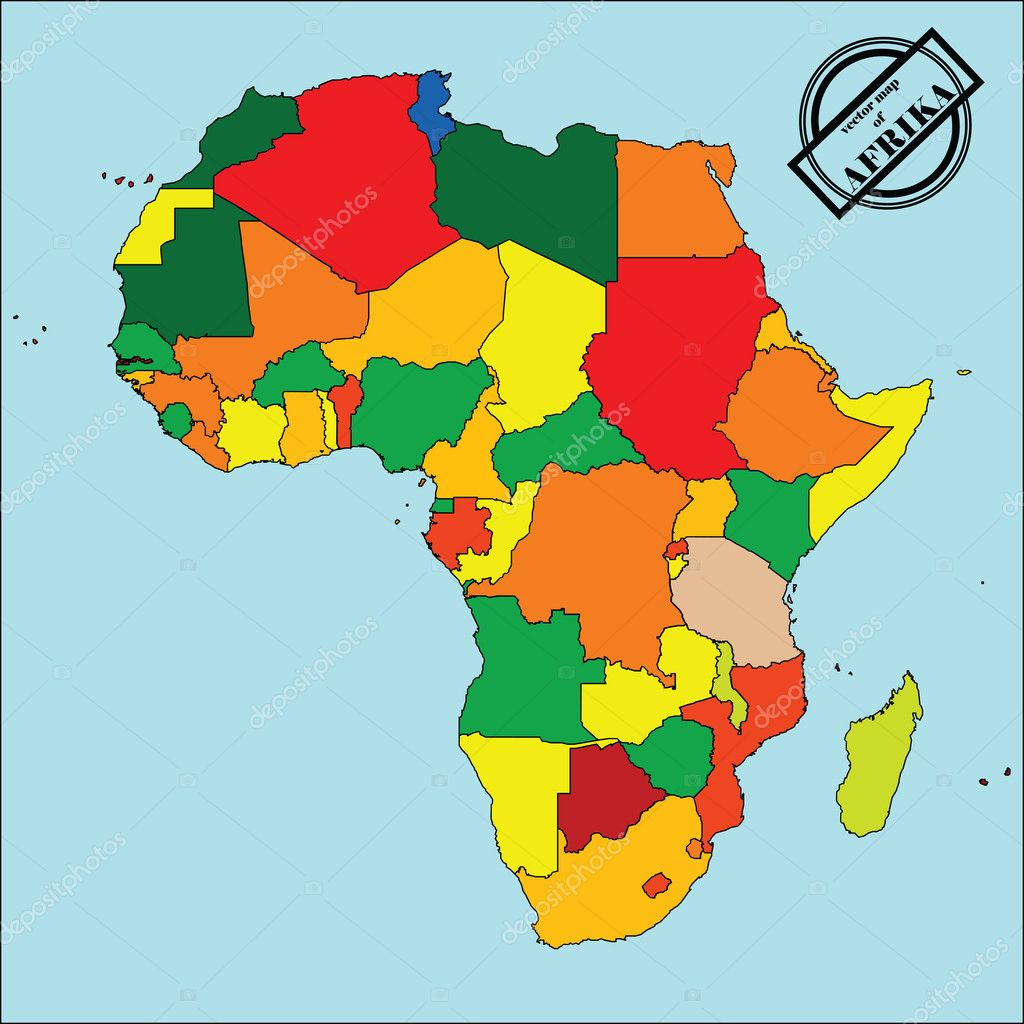
\includegraphics[width=0.4\textwidth]{worldMap_Africa.jpeg}};

\node[anchor=south west] (TMM_2022) at ([yshift=+2.0cm]africa.east) {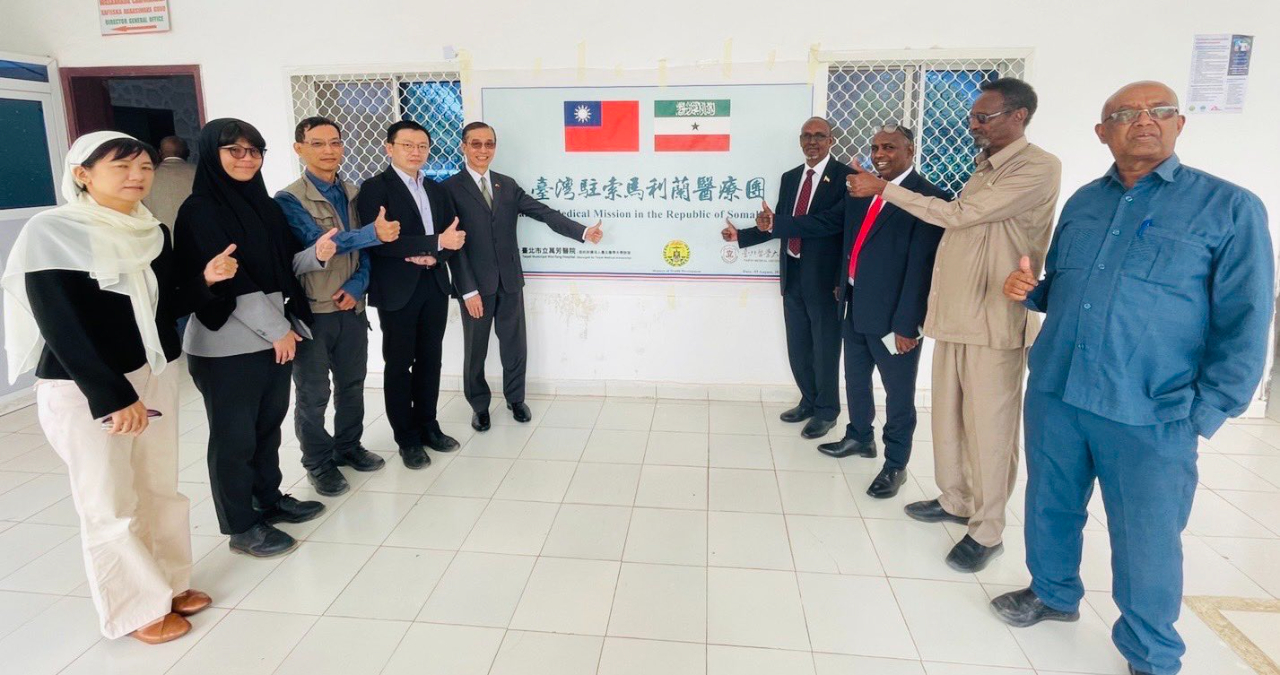
\includegraphics[width=0.30\textwidth]{TMM2022July.jpeg}};

\node[anchor=south west] (TMM_sln) at ([xshift=+4.5cm, yshift=+0.8cm]africa.east) {\includesvg[width=0.14\textwidth]{TMM_logo.svg}};
\node[anchor=west] at (TMM_sln.east) {2022/July};
\draw[green,thick,<-] (4.9,0.55) -- (10.7,1.4);

\node[anchor=north west] (TMM_swati) at ([xshift=+2.0cm, yshift=+0.5cm]africa.east) {
\includegraphics[width=0.15\textwidth]{TMM_Eswatini_logo.jpg}};
\node[anchor=west] at (TMM_swati.east) {2008/Sep};
\draw[blue,thick,<-] (3.95,-1.8) -- (8.2,-1.0);

% Missão Médica de Taiwan (MMT), São Tomé & Príncipe, Gulf of Guinea (Portuguese-speaking)
\node[anchor=south west,align=left,font=\scriptsize\bfseries,text=black] (MMT_stp) at (0.08,-2.55) {Missão Médica\\ de Taiwan\\ (MMT), 2011\\ São Tomé \&\\ Príncipe};
\draw[orange,very thick,<-] (2.15,-0.05) -- ([xshift=4mm]MMT_stp.north);
%\draw (africa.east) -- (TMM_swati.west);
\end{tikzpicture}
\end{frame}

\begin{frame}
\frametitle{Outline}

\begin{columns}
\column{0.4\textwidth}
\tableofcontents

\column{0.6\textwidth}
\includesvg[width=0.7\textwidth]{TMM_logo.svg}

\end{columns}


\end{frame}

\begin{frame}{Key words for today 今日關鍵詞}
\footnotesize
\begin{columns}[t]
\column{0.44\textwidth}
\begin{tabular}{@{}ll@{}}
registered nurse (RN) & 護理師 \\
obstetrics (OBS) & 產科 \\
emergency department (ED) & 急診 \\
intensive care unit (ICU) & 加護病房 \\
operation theatre (OT) & 手術室 \\
antenatal check & 產前檢查 \\
home visit & 居家訪視 \\
capacity building & 能力建構 \\
\end{tabular}
\column{0.56\textwidth}
\begin{tabular}{@{}ll@{}}
public health & 公共衛生 \\
Pap smear & 子宮頸抹片 \\
blood donor & 捐血者 \\
non-communicable disease (NCD) & 非傳染性疾病 \\
point-of-care ultrasound & 床邊超音波 \\
trauma kit & 創傷急救包 \\
telepathology & 遠距病理 \\
IDP (internally displaced persons) & 境內流離失所者 \\
\end{tabular}
\end{columns}
\end{frame}


%%%%%
\section{Overture}

\begin{frame}{Overture 序曲}
    \begin{center}
        \includesvg[width=0.8\textwidth]{TRO_Somaliland_font_ZongKai.svg}
    \end{center}
\end{frame}

\begin{frame}{Overture 序曲}

\begin{columns}[c]
\column{0.62\textwidth}
{\small
\pl{Here is the diplomatic vanguard of the Republic of China (Taiwan);}{這裡是中華民國的外交先鋒，}
\pl{here is Somaliland's support behind the front line;}{這裡是索蘭的戰地後盾，}
\pl{here looks like Taiwan in the 1970s.}{這裡像是，1970年代的臺灣，}
\pl{We were not part of Taiwan's past,}{我們沒有參與過去的臺灣，}
\pl{but we are writing Somaliland's medical history.}{但我們正在撰寫索蘭的醫療史，}
\pl{The Taiwan Medical Mission:}{Taiwan Medical Mission 是，}
\pl{\textbf{unarmed heroes behind the scenes.}}{不拿槍的幕後英雄。}
}

\column{0.38\textwidth}
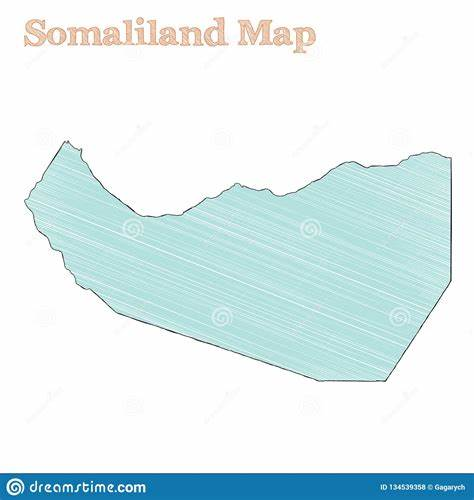
\includegraphics[width=0.95\textwidth]{Somaliland.jpeg}
\end{columns}

\end{frame}




%%
\section[Q\&A]{Students' Q\&A}
% Questions asked by Taiwanese students at an earlier talk (2023); names and times removed for this EMI version.

\begin{frame}{Q1. Working with other countries}
\textbf{Q:} Over the years, have other countries worked with you? \\
{\footnotesize\color{gray}問：這麼多年，有其他國家與你們合作嗎？}

\vspace{0.8em}
\textbf{A:} Yes. In the field, our mission runs projects together with WHO and with NGOs from the UK, the USA, Australia and others. \\
{\footnotesize\color{gray}答：我們醫療團會在駐地，與WHO、英、美、澳洲等 NGO 合作推動計畫。}
\end{frame}

\begin{frame}{Q2. What help is useful for Somaliland?}
\textbf{Q:} What kind of help from other countries is useful for health care in Somaliland? \\
{\footnotesize\color{gray}問：其他國家給予什麼樣的協助對於索馬利蘭的醫療發展是有幫助的？}

\vspace{0.8em}
\textbf{A:} For example: hepatitis vaccines, UNICEF maternal and child health, and safe water. In 2024 our mission ran dengue fever prevention and women's health (Pap smear and breast cancer screening). \\
{\footnotesize\color{gray}答：例如肝炎疫苗、UNICEF婦幼保健、安全用水，今年度(2024)我們醫療團則推行登革熱防治工作，以及婦女健康（子宮頸抹片、乳癌篩檢）。}
\end{frame}

\begin{frame}{Q3. Where can Taiwan help more?}
\textbf{Q:} In which areas of health care can Taiwan offer more help? \\
{\footnotesize\color{gray}問：台灣在醫療的哪一方面還能提供更多什麼幫助？}

\vspace{0.8em}
\textbf{A:} Every area. We started with maternal and child health, orthopaedics and surgery, plus hepatitis vaccines, dengue and the cervical HPV vaccine. \\ But some cases are no longer seen in Taiwan, and there \textcolor{red}{we learn from them}: open gallbladder surgery, cleft lip and palate, imperforate anus, gunshot wounds, very difficult deliveries. \\
{\footnotesize\color{gray}答：全面都行。而目前先由婦幼、骨科、外科開始，以及肝炎疫苗、登革熱、子宮頸HPV疫苗。但是，有些手術在臺灣已經看不到了，倒是我們要向他們學習（膽囊open surgery、先天性唇顎裂、無肛門症、槍傷，非常困難的生產）。}
\end{frame}

\begin{frame}{Q4. Is it safe?}
\textbf{Q:} Is Somaliland safe compared with other countries? \\
{\footnotesize\color{gray}問：東非索馬利蘭這個國家治安相較於其他國家好嗎？}

\vspace{0.8em}
\textbf{A:} Relatively safe (compared with South Africa or Central America), about the same as Eswatini in southern Africa. \\ Update: in May 2026, President Lai of the ROC (Taiwan) visited Eswatini; on 10 October 2026 (ROC National Day), King Mswati III of Eswatini visited Taiwan for the celebration. \\
{\footnotesize\color{gray}答：相對安全（與南非、中美洲比），與南部非洲的史瓦濟蘭（史瓦帝尼）差不多。補充：2026 年 5 月，中華民國賴總統訪問史瓦帝尼；10 月 10 日國慶，史瓦帝尼國王恩史瓦帝三世訪臺同慶。}
\end{frame}

\begin{frame}{Q5. Who fits a medical mission in Africa?}
\textbf{Q:} What personal qualities or experience do you need to join a medical mission in Africa? \\
{\footnotesize\color{gray}問：有什麼樣特質的人或有什麼資歷可以到非洲醫療團？}

\vspace{0.8em}
\textbf{A:} \textcolor{red}{Compassion and empathy}; you like making friends; you adapt to whatever comes --- and you are fine without (Asian) Taiwanese food. \\
{\footnotesize\color{gray}答：有愛心、同理心、愛交朋友，能隨遇而安，而且若沒有(亞洲)臺灣食物也無所謂。}
\end{frame}

\begin{frame}{Q6. Was daily life hard?}
\textbf{Q:} Was life there hard to adjust to? \\
{\footnotesize\color{gray}問：在那邊的生活會不會有不適應的地方？}

\vspace{0.8em}
\textbf{A:} When I arrived in July 2022: wow --- stone and sand roads everywhere; paved roads were rare and full of potholes. \\ (Dr. Andrew: no air conditioning, and at noon it is hot \ldots\ 35\,$^\circ$C.) \\
{\footnotesize\color{gray}答：2022/07 抵達時：哇怎麼都是石頭路與沙地，柏油路少見，也滿佈坑洞。(Dr. Andrew: 都沒有冷氣機，中午好熱....35 degree C)}
\end{frame}

\begin{frame}{Q7. Advice for future volunteers}
\textbf{Q:} Any advice for students who want to become international medical volunteers? Do I need strong medical knowledge first? \\
{\footnotesize\color{gray}問：對以後有想去當國際醫療志工的人有沒有什麼建議，例如：需要先具備良好的醫學知識等？}

\vspace{0.8em}
\textbf{A:} Start building international experience in \textcolor{red}{student groups} now; diplomatic alternative military service is a good option. To join a medical mission, first gain experience as a \textcolor{red}{registered nurse} or a specialist doctor. \\ English is not hard: living in an English environment, your listening grows fast. \\
{\footnotesize\color{gray}答：學生團體就能開始累積國際經驗，外交替代役男是個好主意，至於醫療團，要等到護理師、專科醫師有經驗之後囉。英語的聽說寫不困難，因為身處英語環境，聽力自然會大幅成長。}
\end{frame}




%%
\section{Introduction}
\begin{frame}
\frametitle{Introduction}
% Add content here
\begin{outline}
    

\1 The Taiwan Medical Mission (TMM) is an overseas project that helps the people of Somaliland get health care since 2022/07/28.
    \2 our brother mission: TMM in the Kingdom of Eswatini since 2008 led by Dr. Tu Chi-cheng (杜繼誠團長)
\1 The team consists of % 程書螢 林威霖 巫昀祐 黃郁昕
    \2 an obstetrician (David/YuHsin), a registered nurse (Josh/Penny), a general surgeon doctor (Andrew), an emergency doctor (Hsu), and an oral and maxillofacial surgeon (Jamal Tex); a administrator (Cecilia/Amui). 
    \2 to support medical staffs who work at the Hargeisa Group Hospital (HGH), Hargeisa, Somaliland
%\1 TMM members are willing to adapt to different cultures and settings and work with limited resources and facilities.



\end{outline}

\qrcode[height=0.7in]{https://youtu.be/uOwzikPw-0U}
2023/05 TV documentary: 消失的國界 (SET TV, East Africa)

\end{frame}


\begin{frame}{Medical affairs --- on TV (消失的國界)}
    \begin{center}
        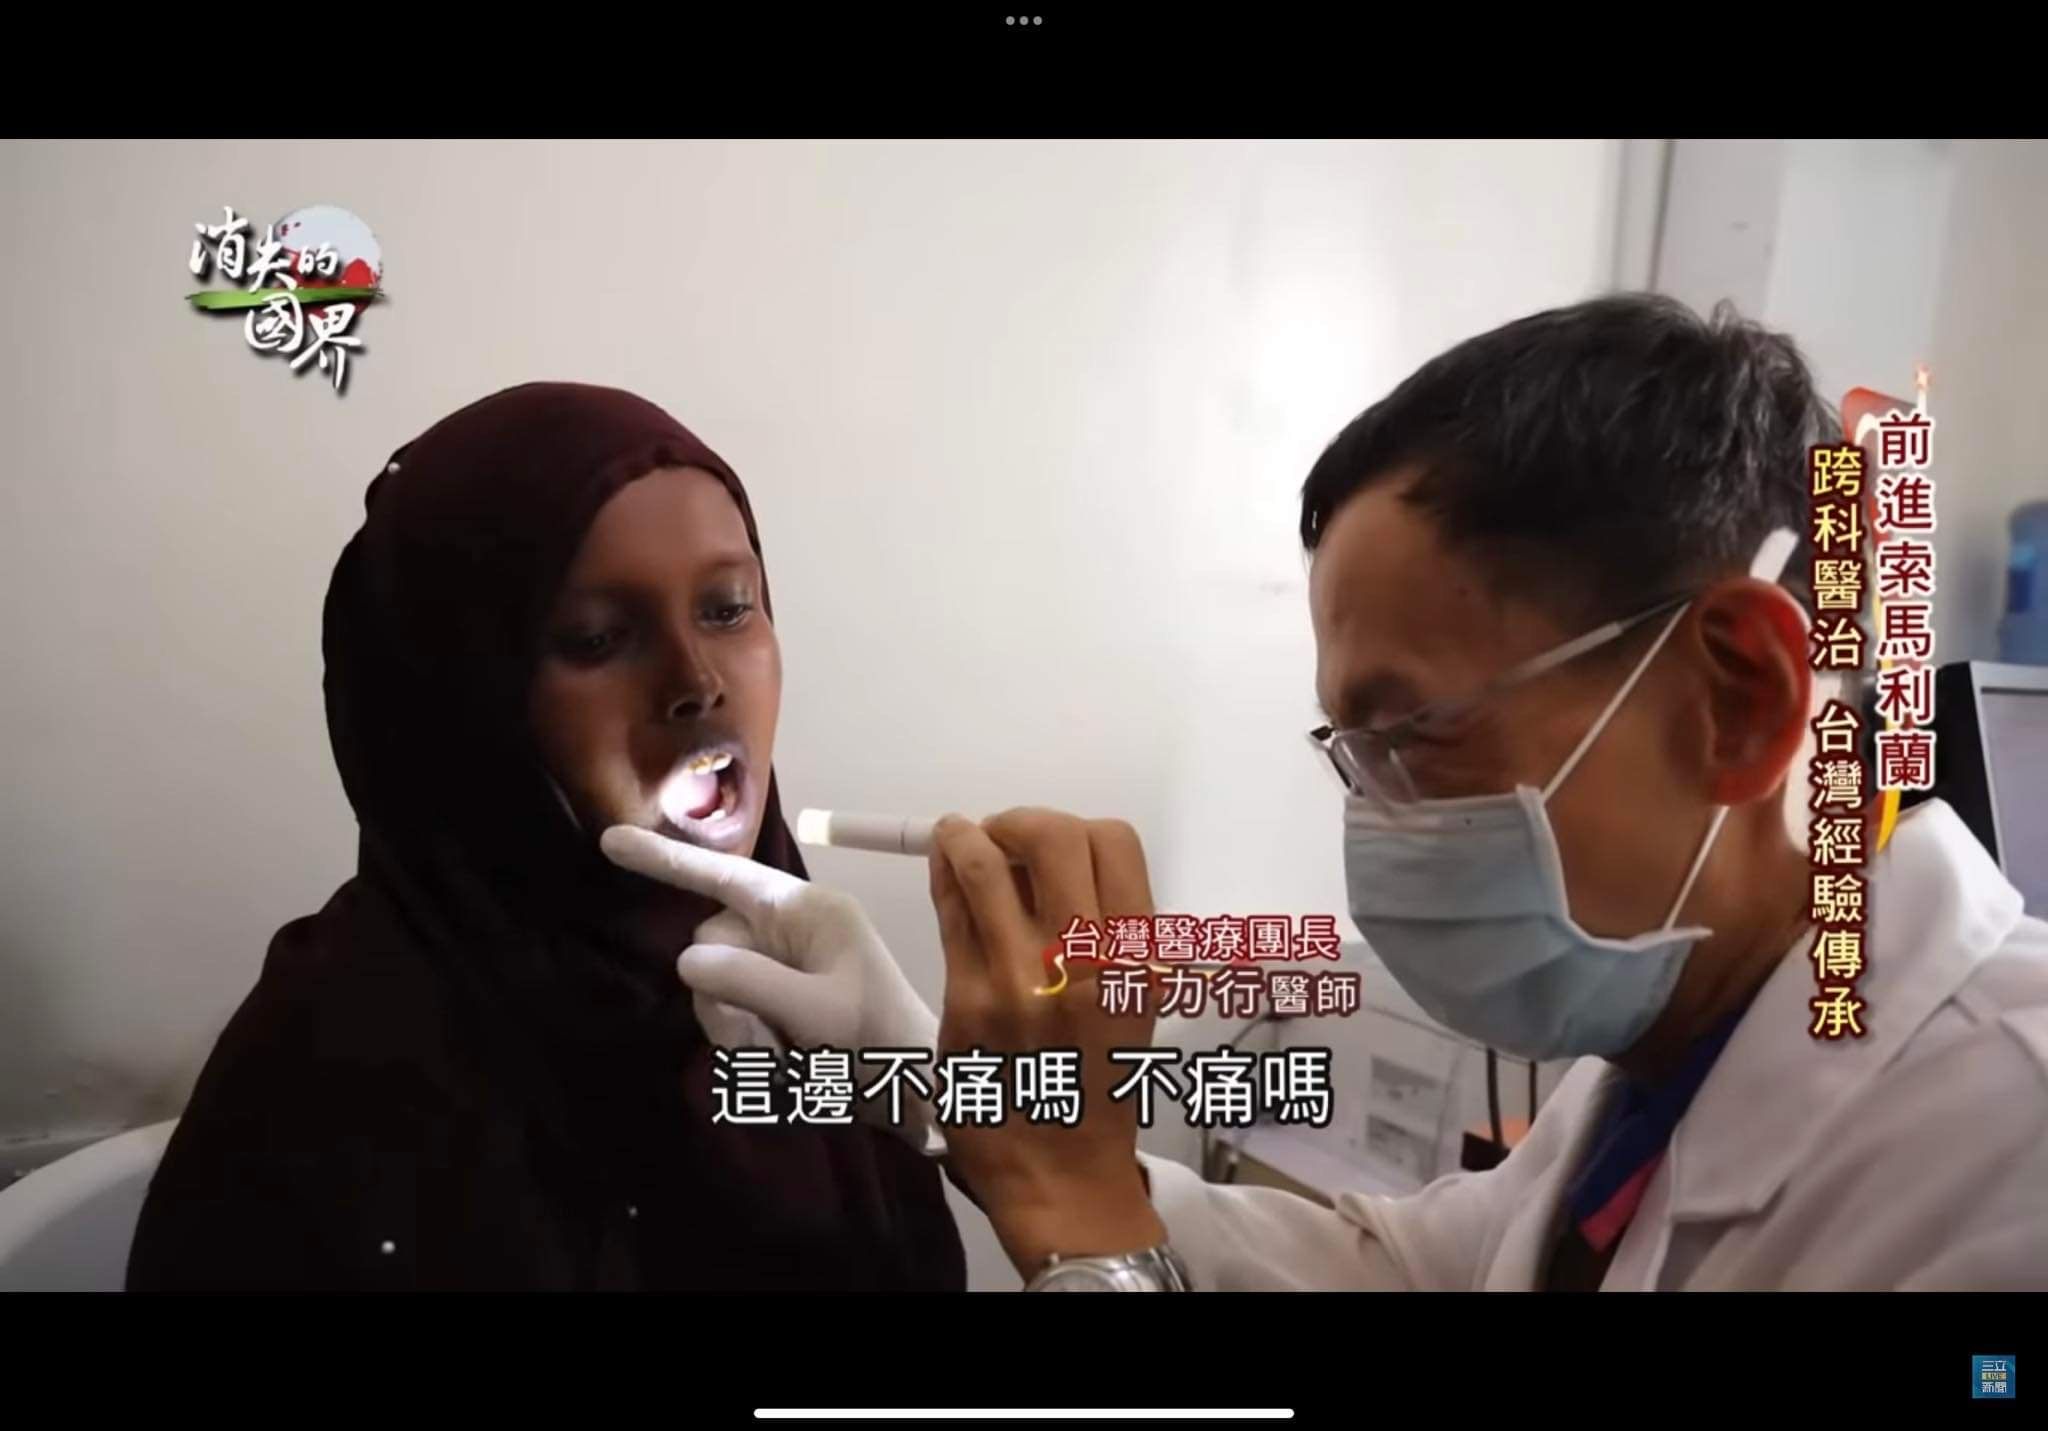
\includegraphics[width=0.8\textwidth]{IMG_4940(1).jpeg}

    \end{center}
\end{frame}

\begin{frame}{Medical affairs --- on TV (消失的國界)}
\begin{center}
    
\begin{tikzpicture}
    \node[anchor=south west,inner sep=0] (image) at ($(current page.center)+(-2cm,0)$) {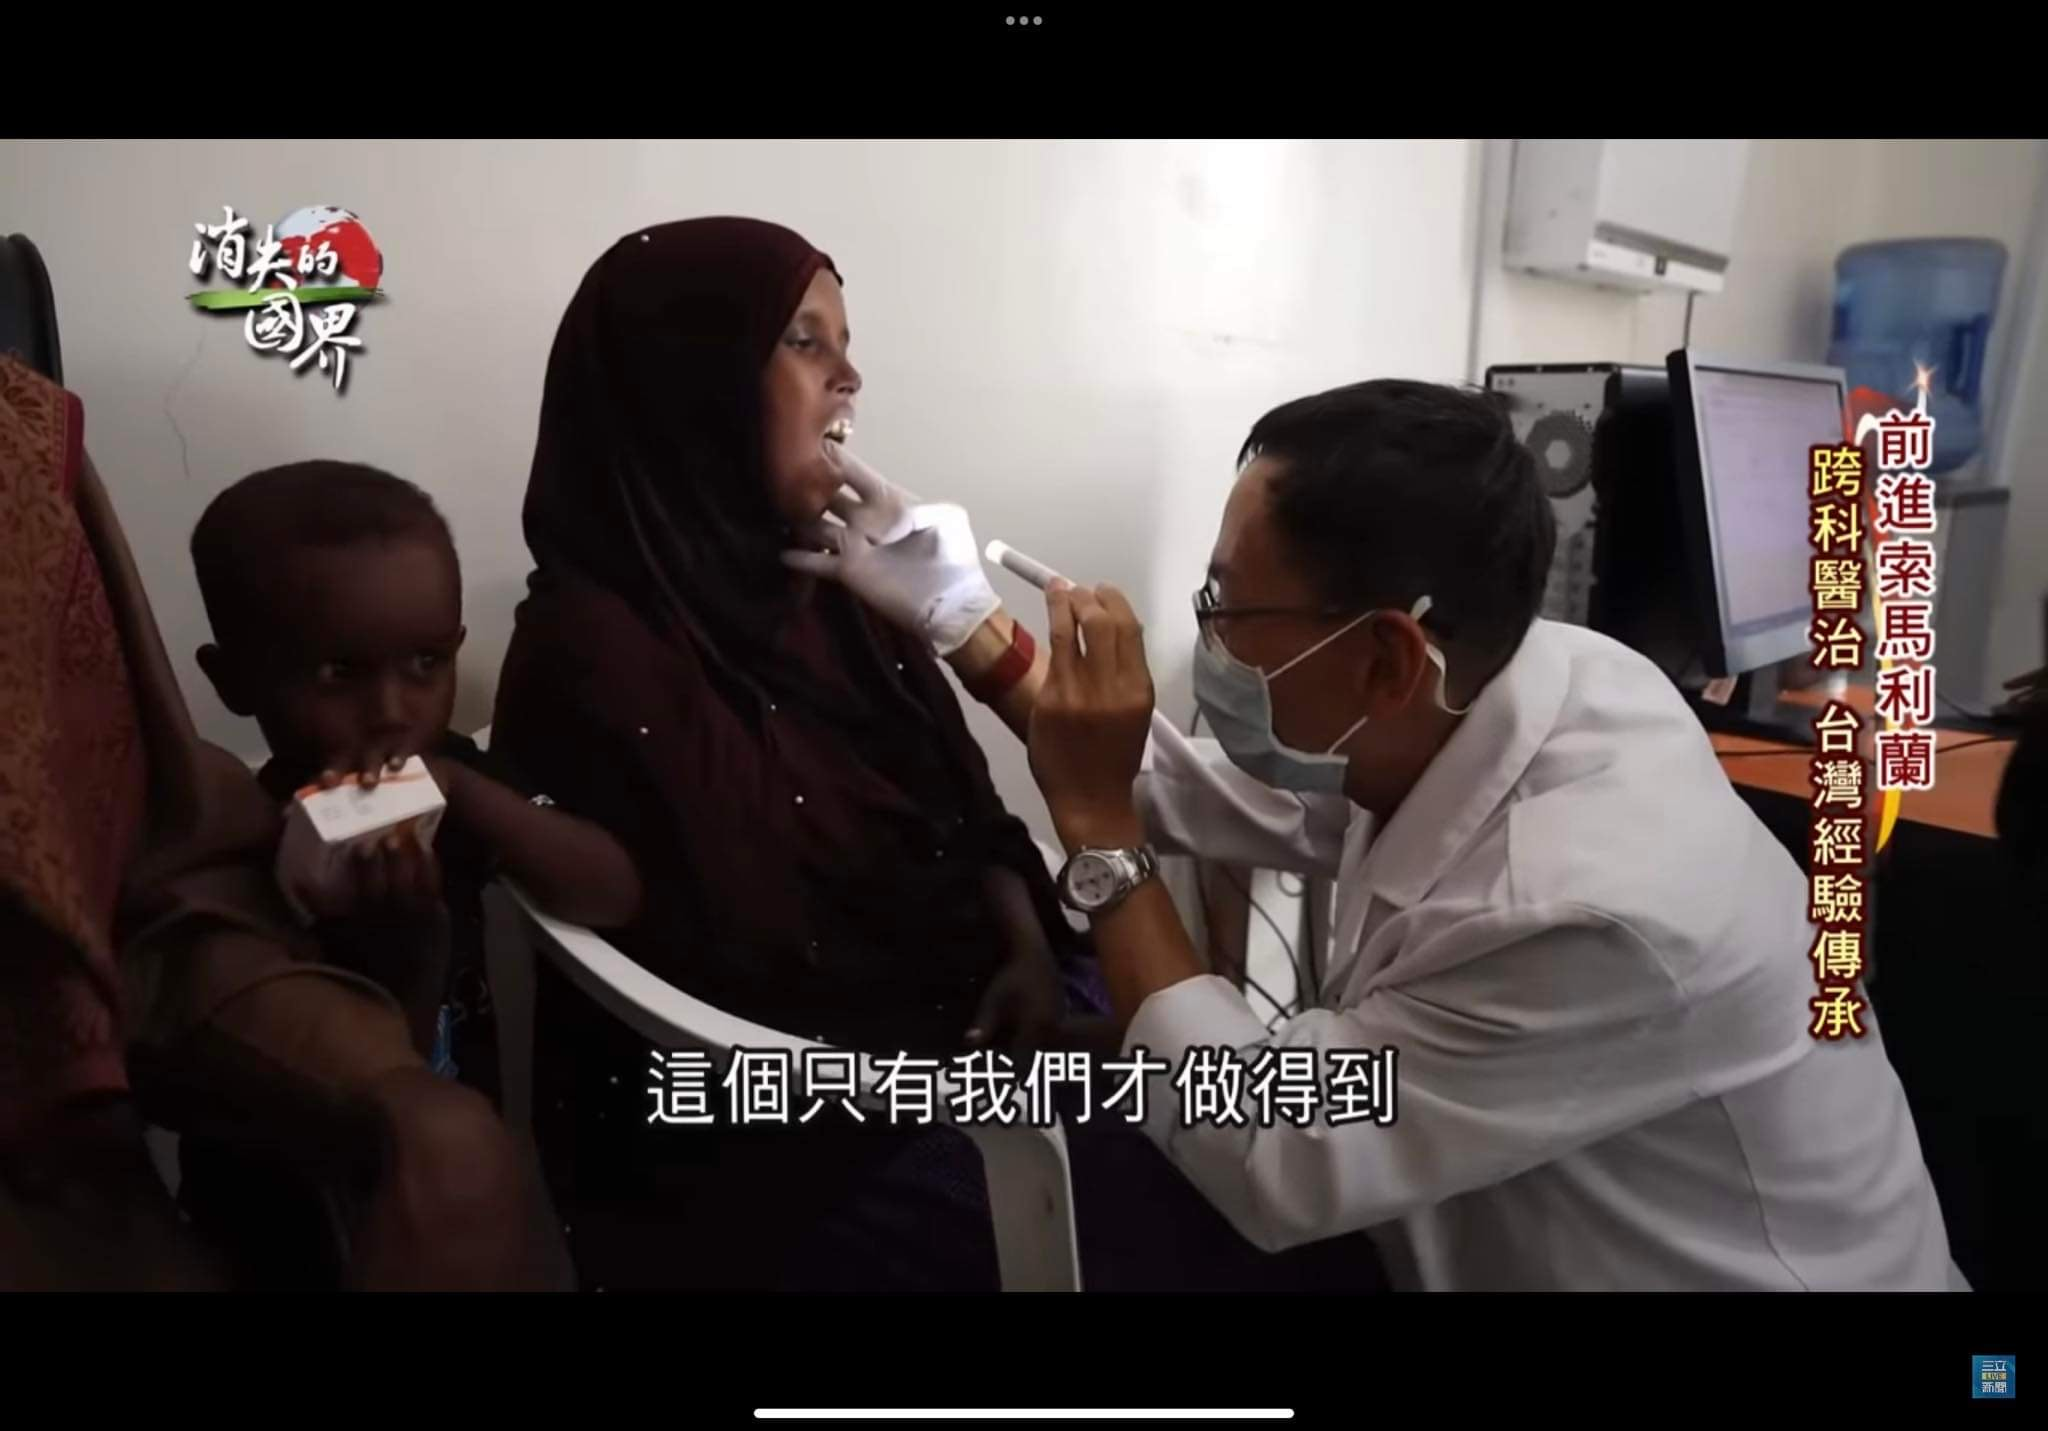
\includegraphics[width=0.8\textwidth]{IMG_4949(1).jpeg}};
    \begin{scope}[x={(image.south east)},y={(image.north west)}]
        \fill[white] (0.25,0.60) circle (0.04);
    \end{scope}
\end{tikzpicture}

\end{center}

\end{frame}


\begin{frame}{Islamic Africa}

\begin{outline}
    \1 TMM members are willing to adapt to Muslim's cultures and settings and work with limited resources and facilities.

\end{outline}

\begin{center}
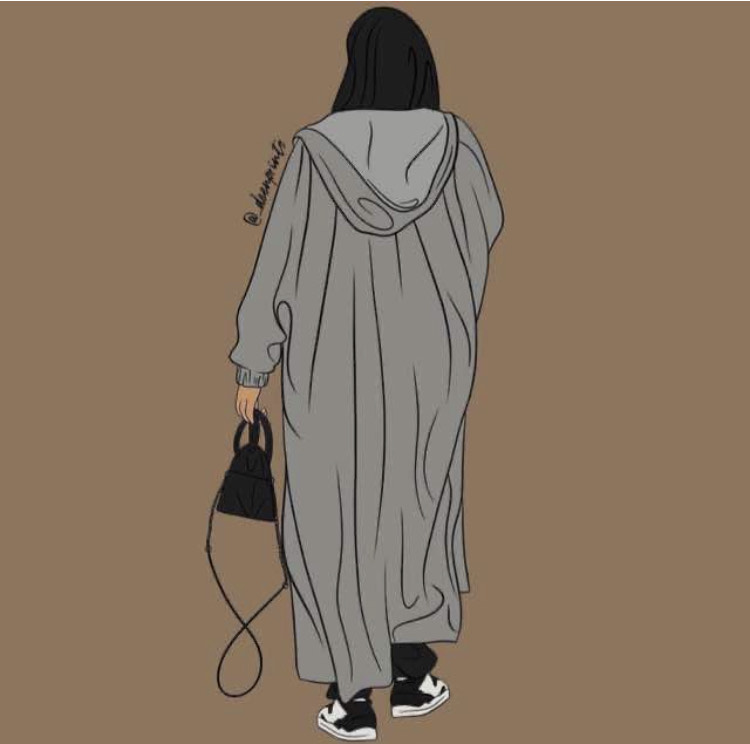
\includegraphics[width=0.23\textwidth]{IMG_4872.jpeg}
\includesvg[width=0.14\textwidth]{anti_CervicalCancer_logo.svg}
\includesvg[width=0.23\textwidth]{Muslim_women_1.svg}
%\includesvg[width=0.14\textwidth]{Muslim_women_2.svg}
%\includesvg[width=0.2\textwidth]{parasite_logo.svg}
\end{center}

\end{frame}
%%%%%%%%%%%%%%%%%%%%%%%%%
\section{Projects}
\begin{frame}
\frametitle{2023 TMM's Projects - first pillar}
% Add content here
\begin{outline}
    TMM is working on a number of projects to improve health care by 1) building capacity, 2) upgrading equipment, 3) implementing screening programs, and 4) working with local health workers and organizations to handle medical affairs.
    
    \1 medical affairs
        \2 Providing quality care to patients through referring to the specialists at TMM
        \2 Working on non-communicable diseases (NCD, such as hypertension, diabetes) together with NGOs
        \2 The point-of-care ultrasound in the emergency department and intensive care unit (ICU) of HGH, Dr. Hsu (TMM) and Dr. Max (from Somalilander-American Healthcare Association, SAHA)

\end{outline}



\end{frame}

\begin{frame}{Medical affairs - trauma ward}
    \begin{center}
        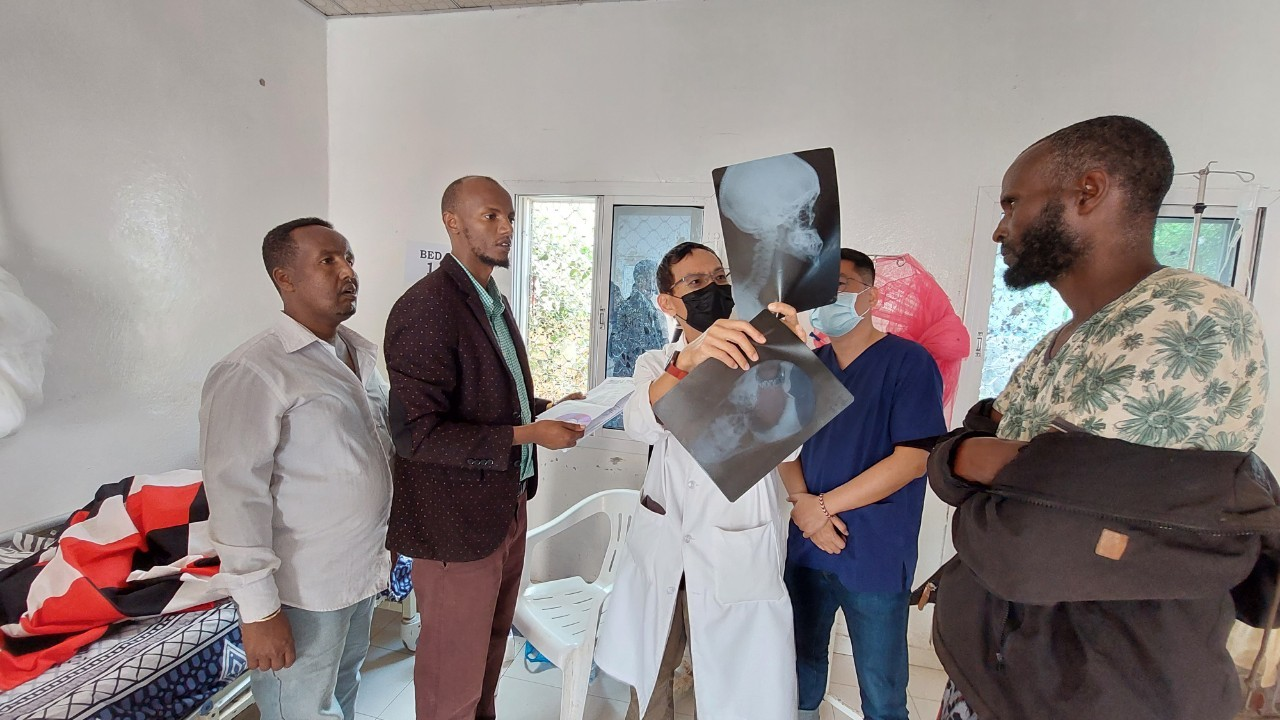
\includegraphics[width=0.8\textwidth]{IMG-4862827583386425169.de8939a35ce768375740b709dce51958.23032108.JPG}
%        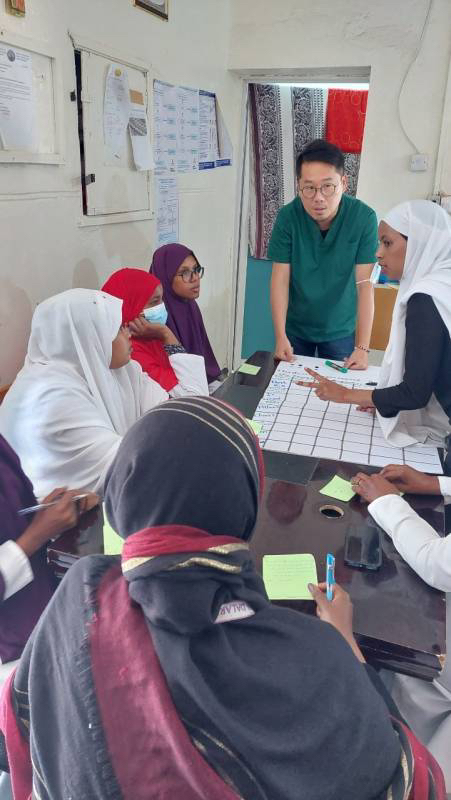
\includegraphics[width=0.2\textwidth]{6963.jpg}
    \end{center}
\end{frame}
    
\begin{frame}{Medical affairs - operation theatre}
    \begin{center}
        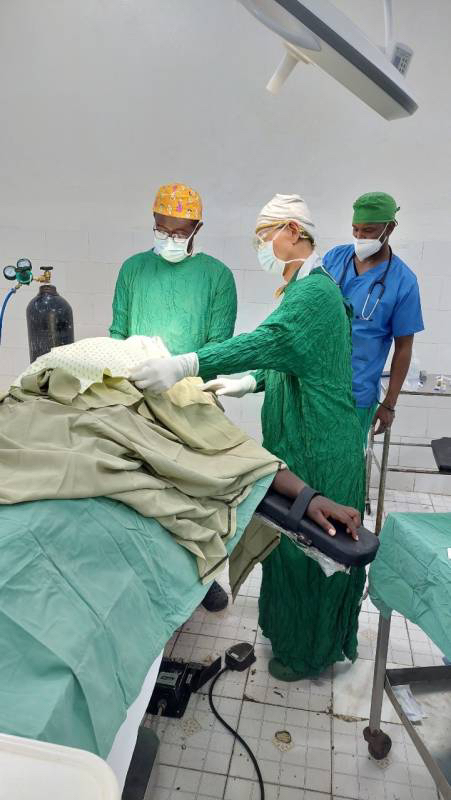
\includegraphics[width=0.35\textwidth]{51744_old_table.jpg}
%        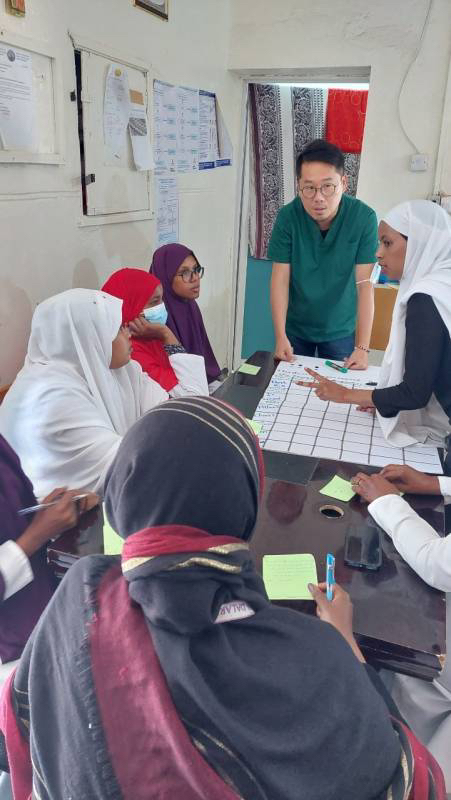
\includegraphics[width=0.2\textwidth]{6963.jpg}
    \end{center}
\end{frame}


\begin{frame}{Medical affairs - OBS, ED}
    \begin{center}
        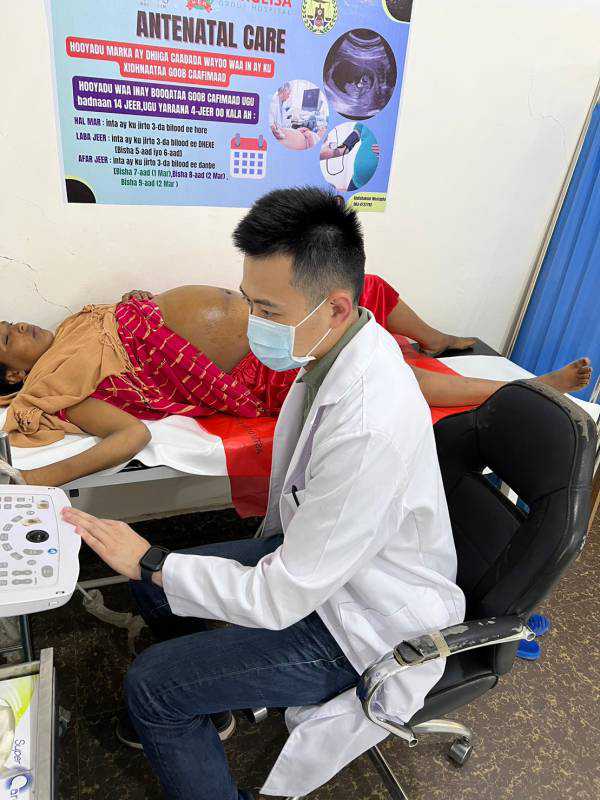
\includegraphics[width=0.25\textwidth, trim=50mm 20mm 40mm 50mm, clip]{52165_antenatal_check.jpg}
        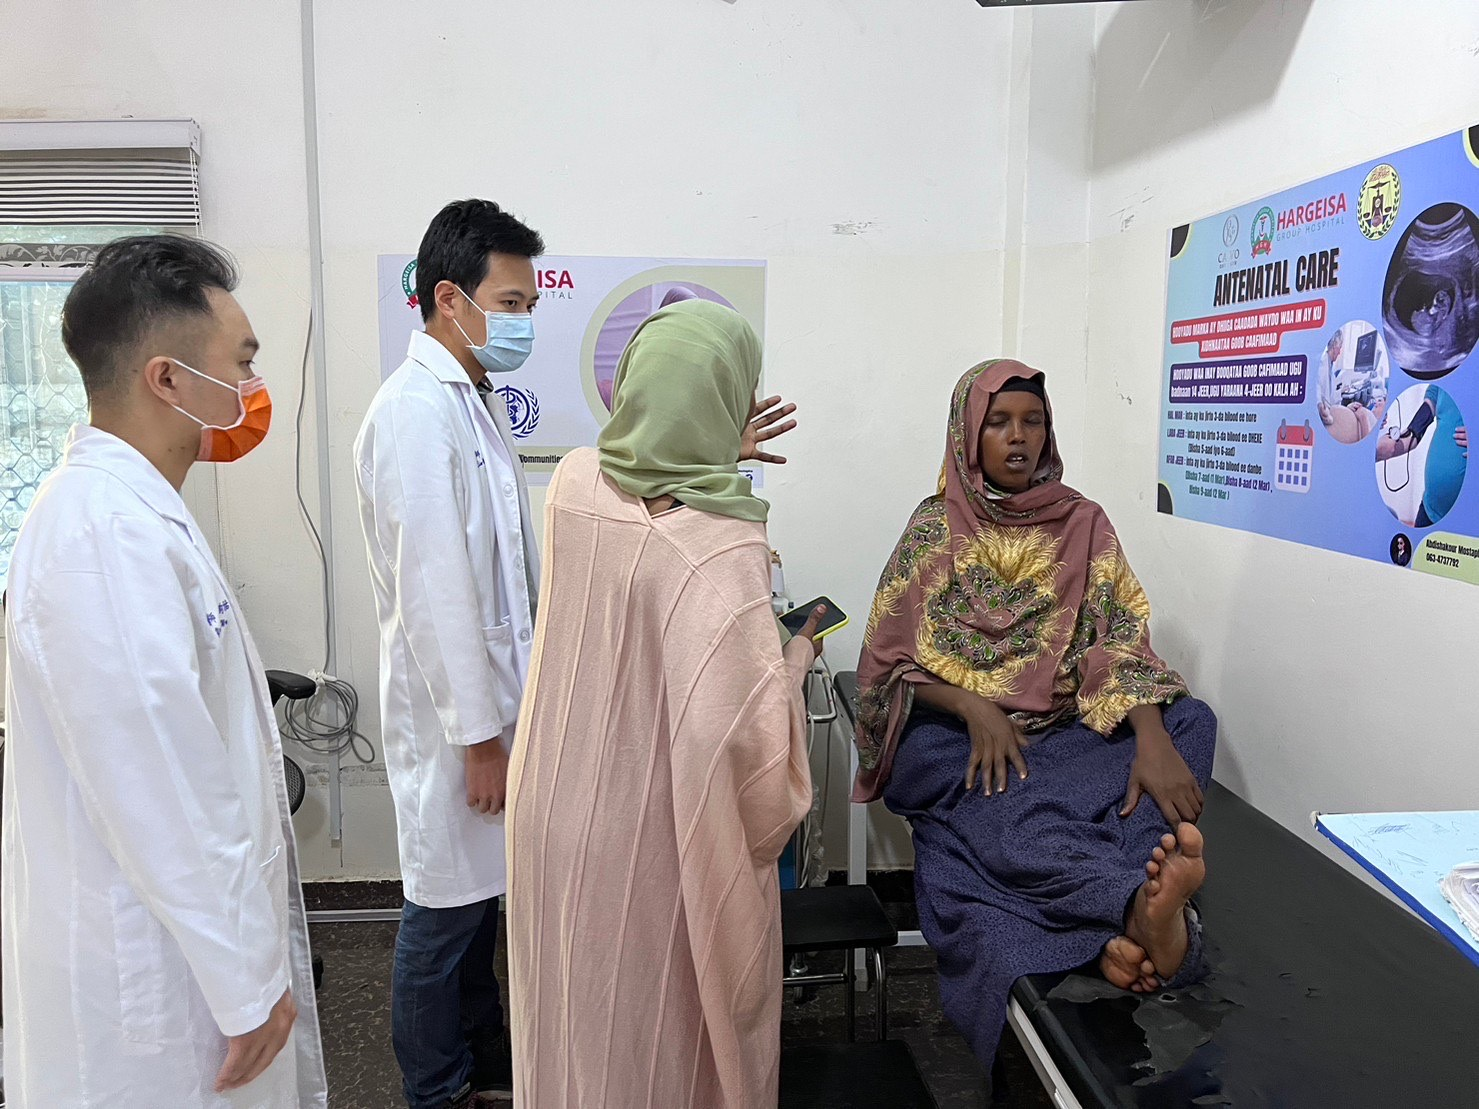
\includegraphics[width=0.4\textwidth]{IMG_5068.jpeg}
    \end{center}
\end{frame}

\begin{frame}{Medical affairs - ED, ward}
\begin{center}
\begin{tikzpicture}
    \node[anchor=south west,inner sep=0] (image) at ($(current page.center)+(0cm,-2cm)$) {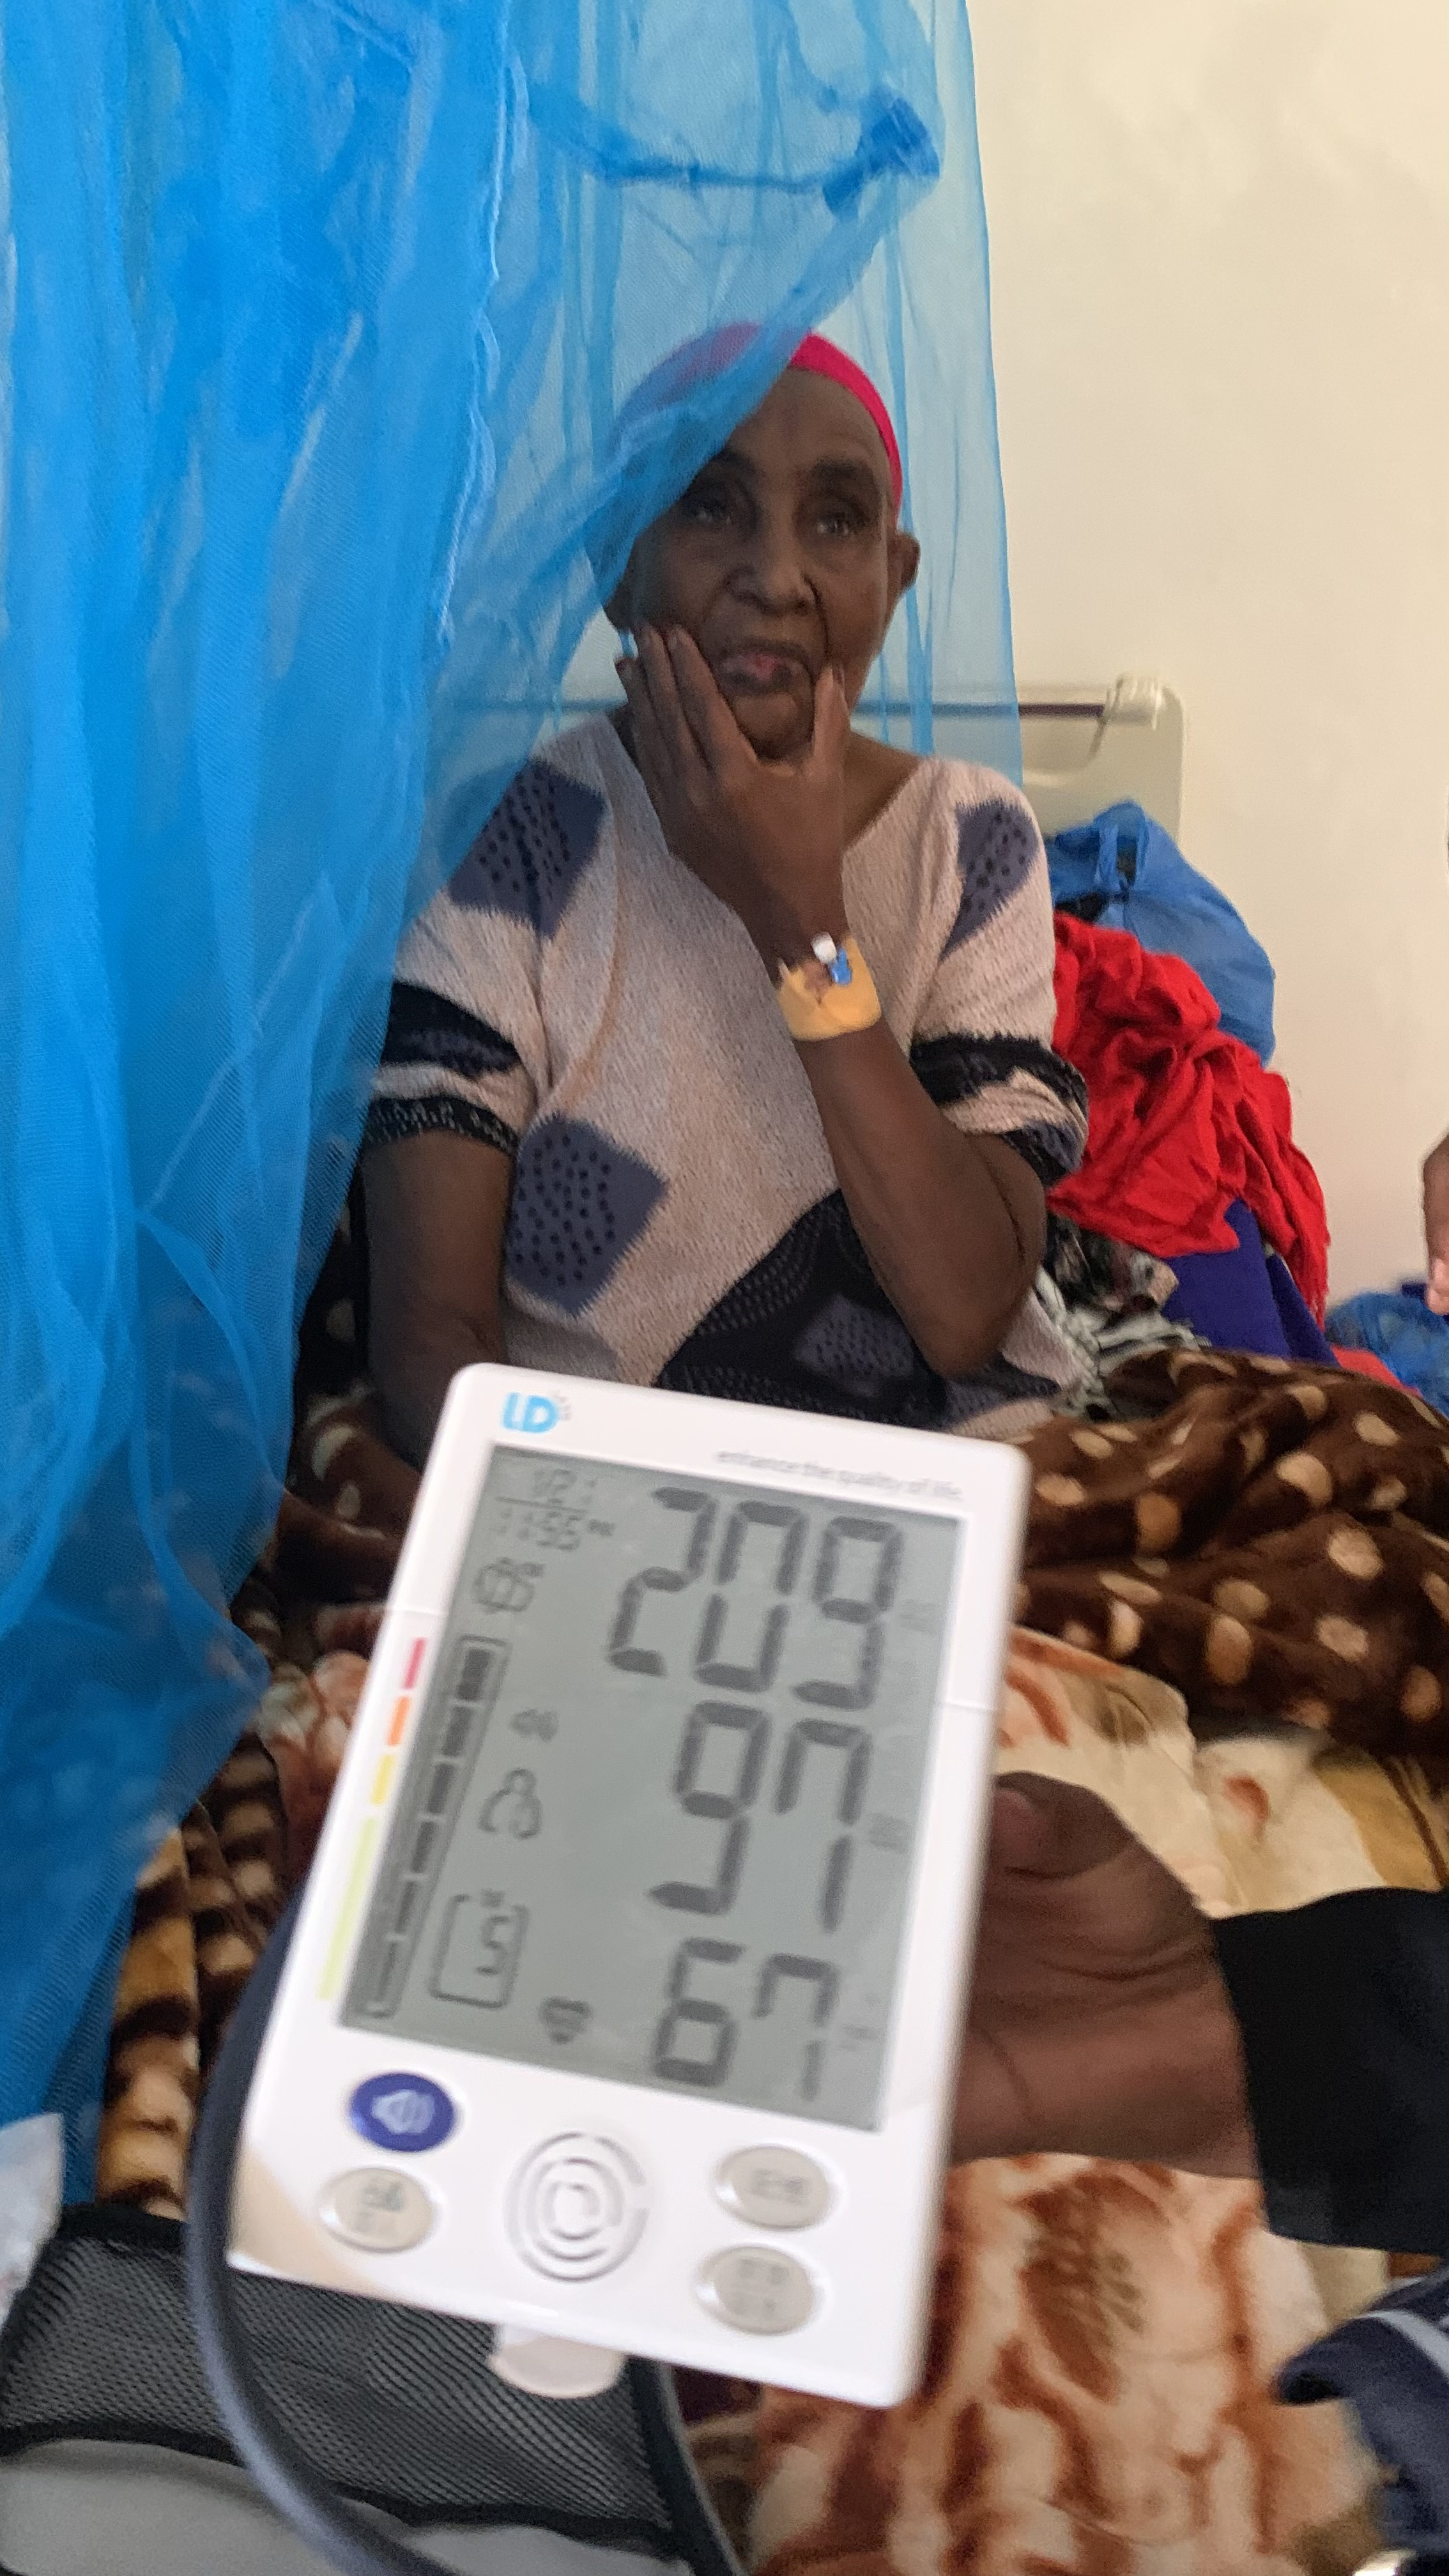
\includegraphics[width=0.30\textwidth]{IMG_5011.jpeg}};
    \begin{scope}[x={(image.south east)},y={(image.north west)}]
        \fill[white] (0.35,0.75) circle (0.03);
    \end{scope}
\end{tikzpicture}

\end{center}
\end{frame}


\begin{frame}{Home visits - OBS, ED}
    \begin{center}
        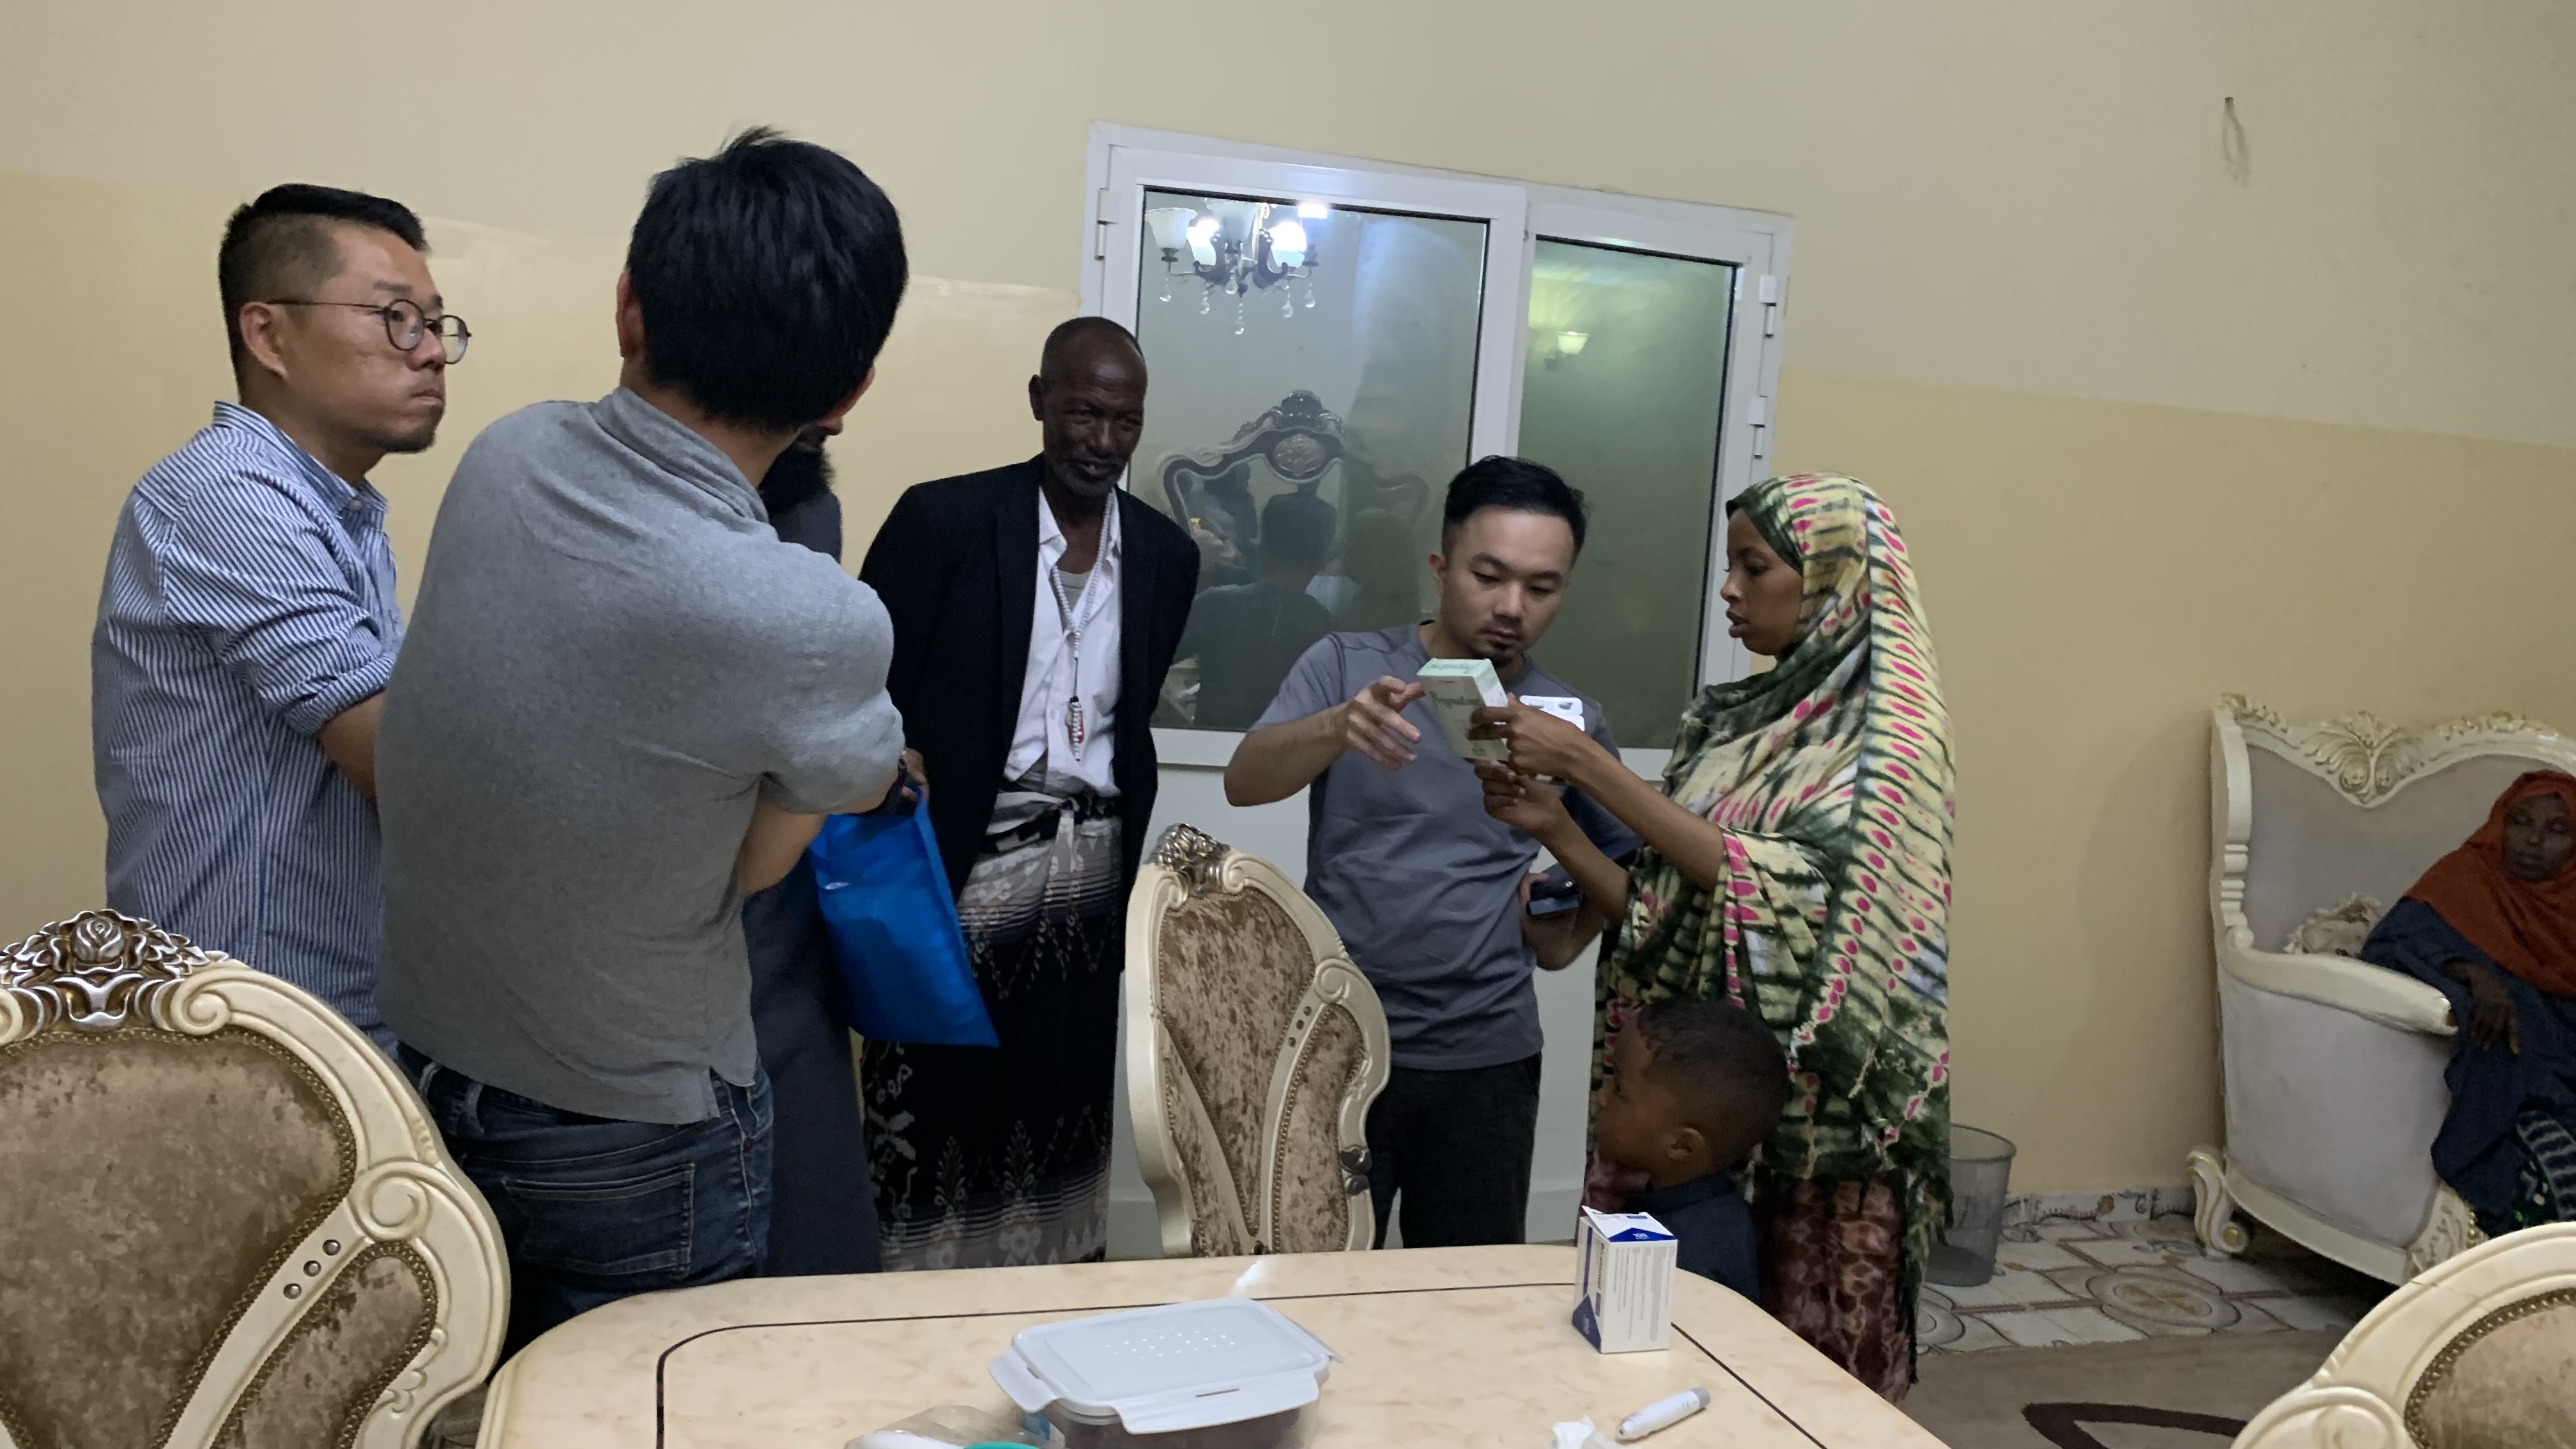
\includegraphics[width=0.55\textwidth]{IMG-5075.jpg}
        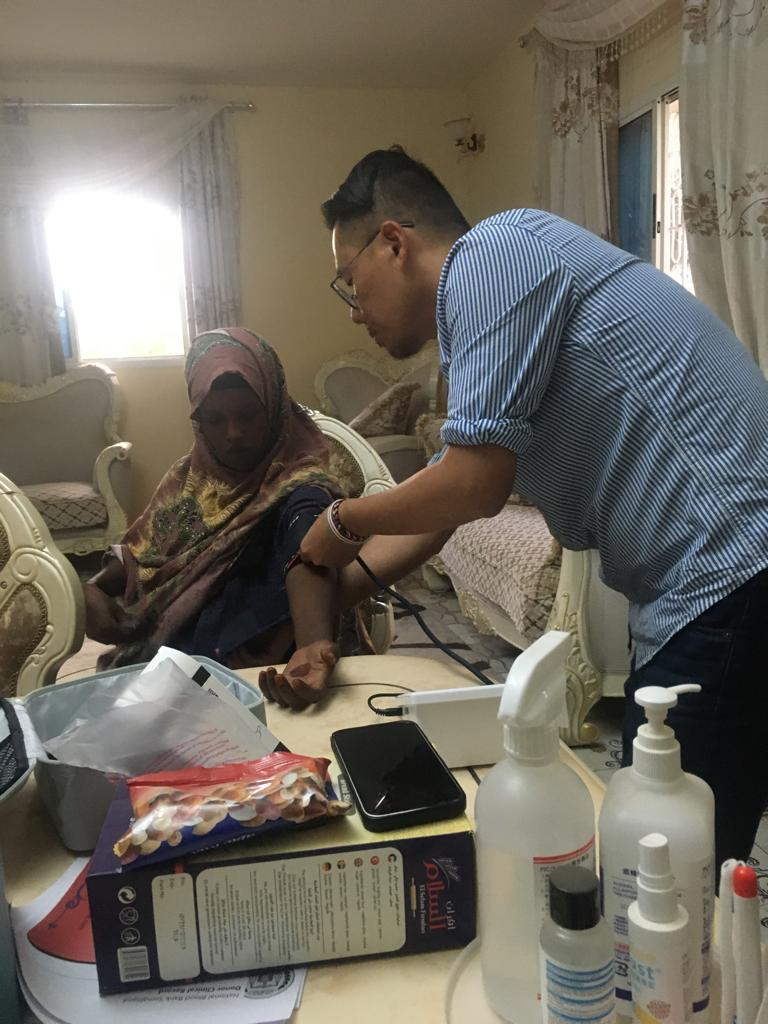
\includegraphics[width=0.25\textwidth]{386eb640-9657-4b71-af5c-5de19cb7b159.JPG}
    \end{center}
\end{frame}


\begin{frame}{Home visits - OMS}
    \begin{center}
        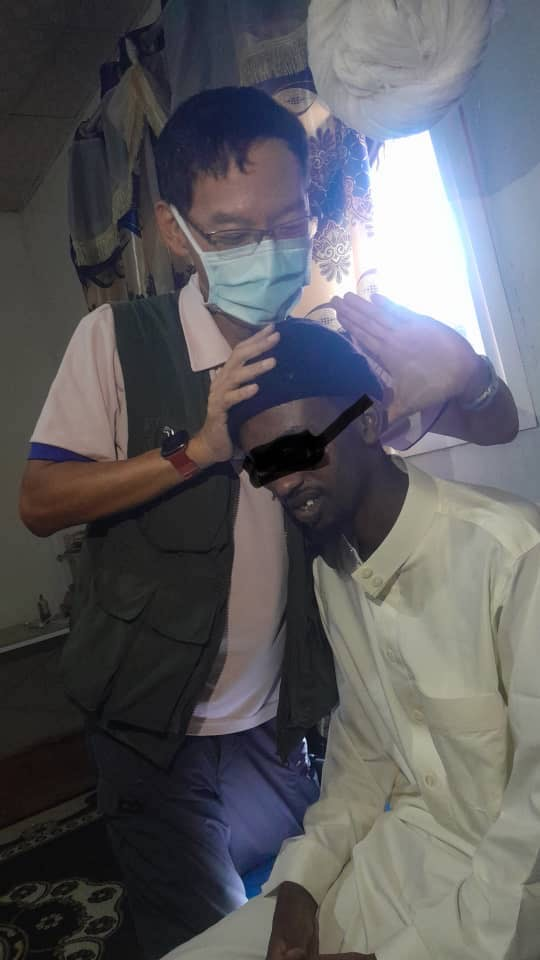
\includegraphics[width=0.20\textwidth]{399223ed-f871-41f7-ae57-c90a5f0ee459.jpeg}
        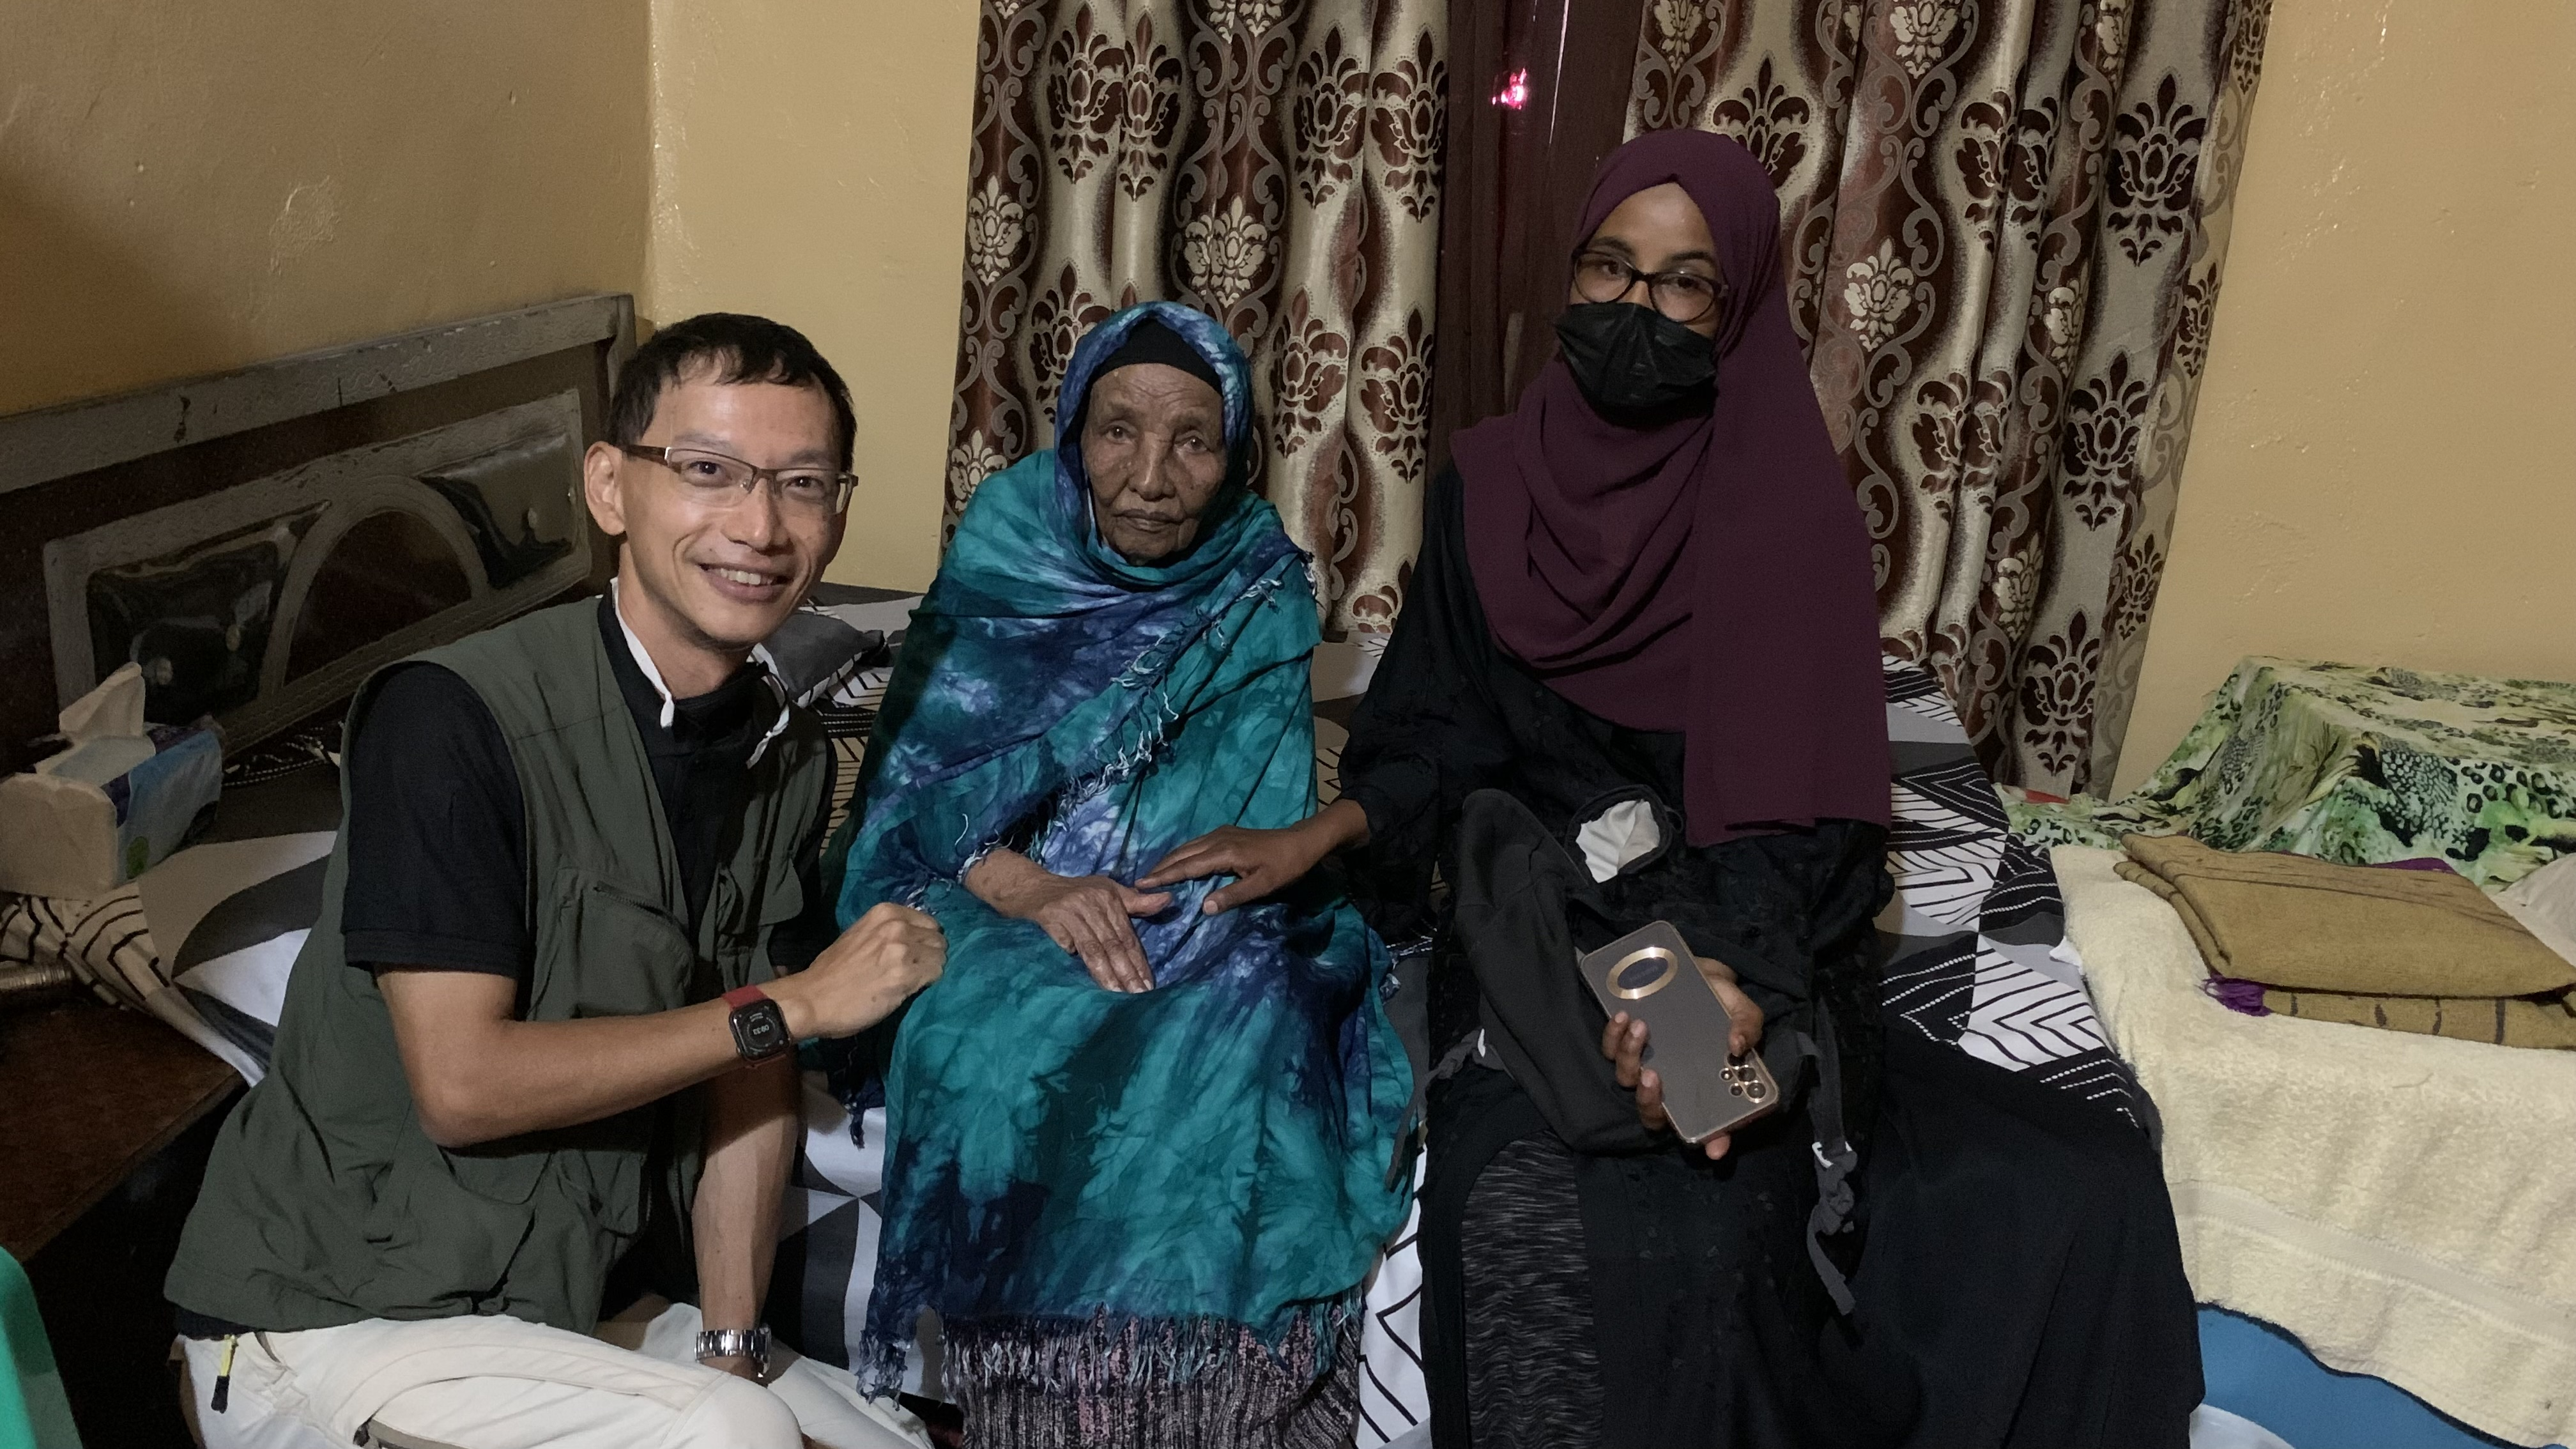
\includegraphics[width=0.50\textwidth]{IMG-3330.jpg}
    \end{center}
\end{frame}




\begin{frame}{Home visits - when doctor becomes patient}
    \begin{center}
        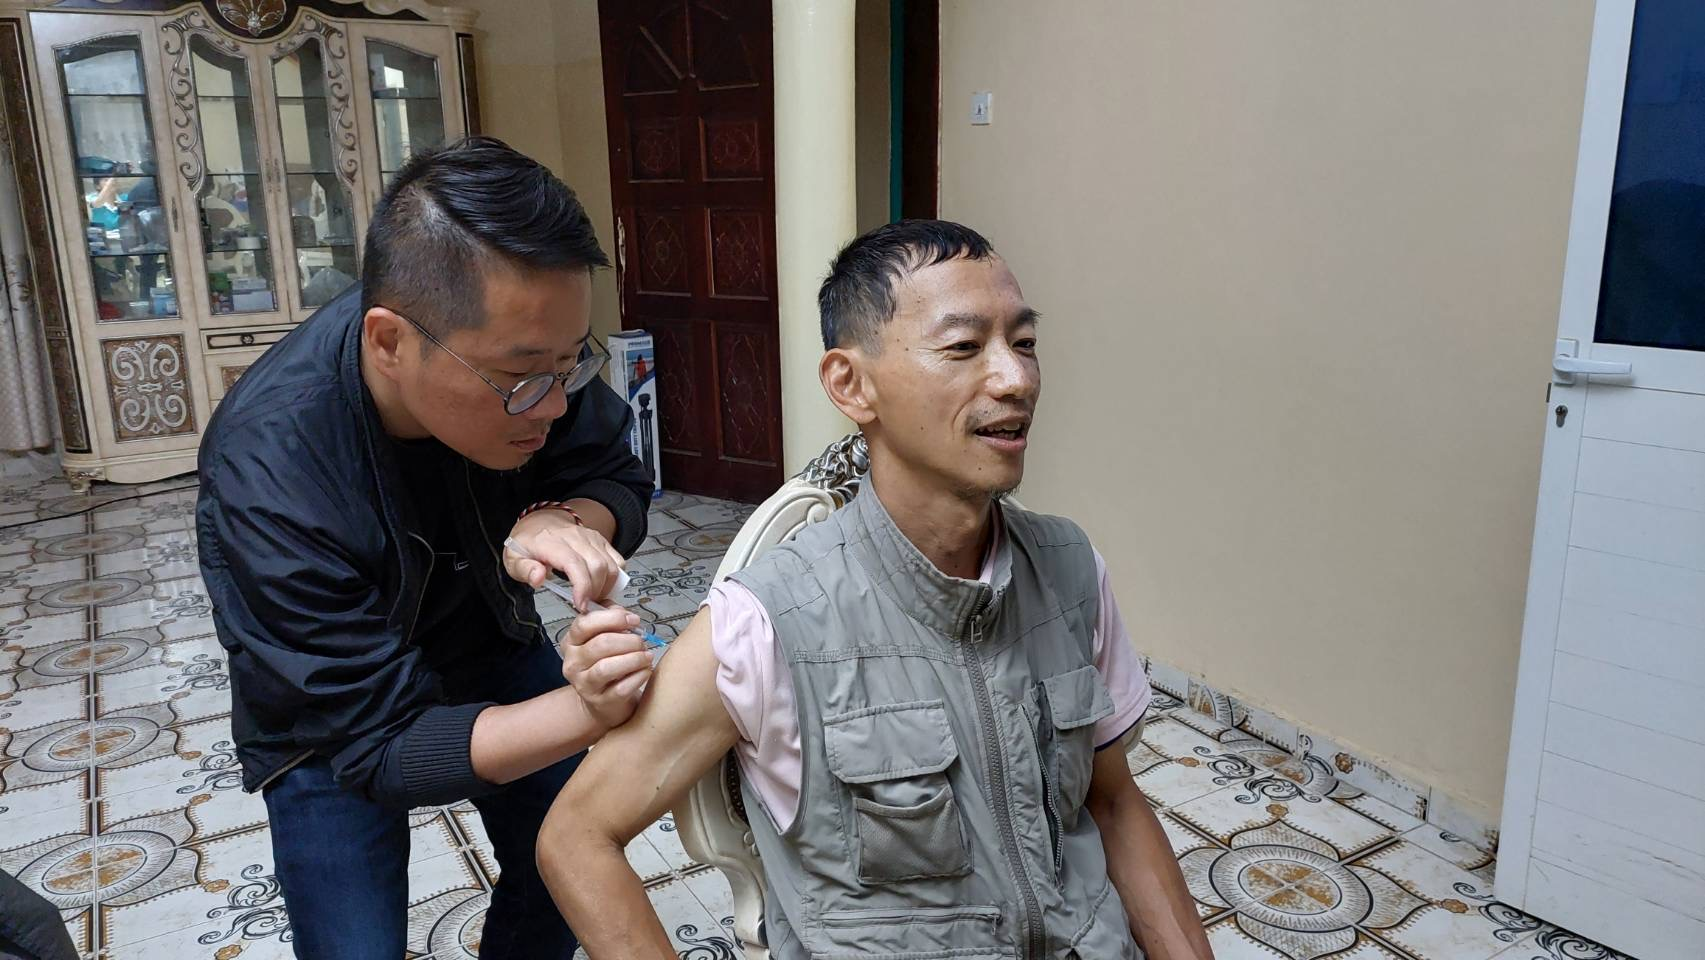
\includegraphics[width=0.50\textwidth]{IMG-2343.JPG}
        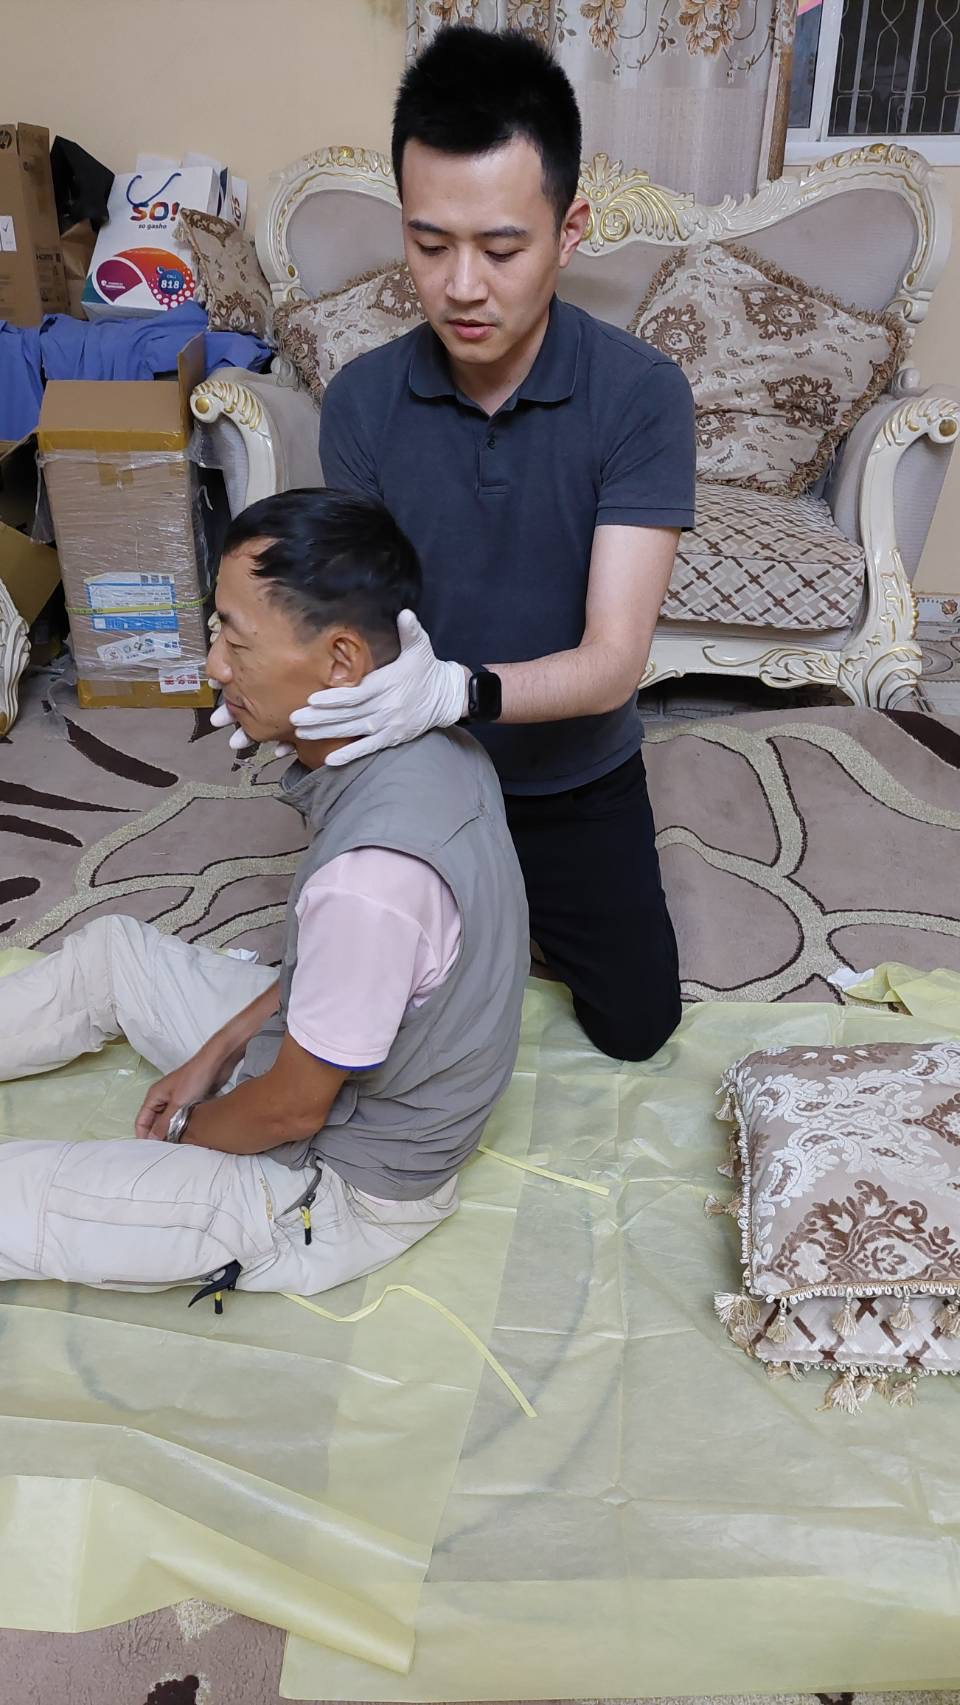
\includegraphics[width=0.20\textwidth]{IMG-2338.JPG}
    \end{center}
    {\small Benign paroxysmal positional vertigo (BPPV, 耳石脫落) gave Dr.~Jamal severe vertigo $\rightarrow$
    manual reduction by Dr.~Lin with the \textcolor{red}{Epley maneuver} (耳石復位：「將機車停好」, ``park the scooter properly'').}
\end{frame}

%%%%
\begin{frame}
\frametitle{TMM's Projects - second pillar}
% Add content here
\begin{outline}    
    \1 capacity building for staffs
        %\2 Contributing to system and equipment upgrades in the orthopedic ward
        \2 \textcolor{red}{On-the-job training} for local doctors to improve their skills and care, in the departments of internal medicine, anesthesiology, orthopedic, obstetricy, emergency, intensive care unit, and maxillofacial surgery in HGH.
        \2 Teaching \textcolor{red}{nurses} basic skills in HGH.        
        \2 Instructing interns at \textcolor{red}{the University of Hargeisa (UoH)}.
        
    \1 capacity building for equipments
        \2 In operation theatre (OT), supporting video intubation system, surgical tables, C-arm X-ray, arthroscopic shaver, maxillofacial/orthopedic instruments/implants, and other \textcolor{red}{medical devices and medicines} for use in HGH.

        \2 Building trauma kits for Somaliland \textcolor{red}{army force}.
        %\2 Assist in establishing department of urology in HGH and their resident training program

\end{outline}
\end{frame}

\begin{frame}{Capacity building: orthopedic}
    \begin{center}
        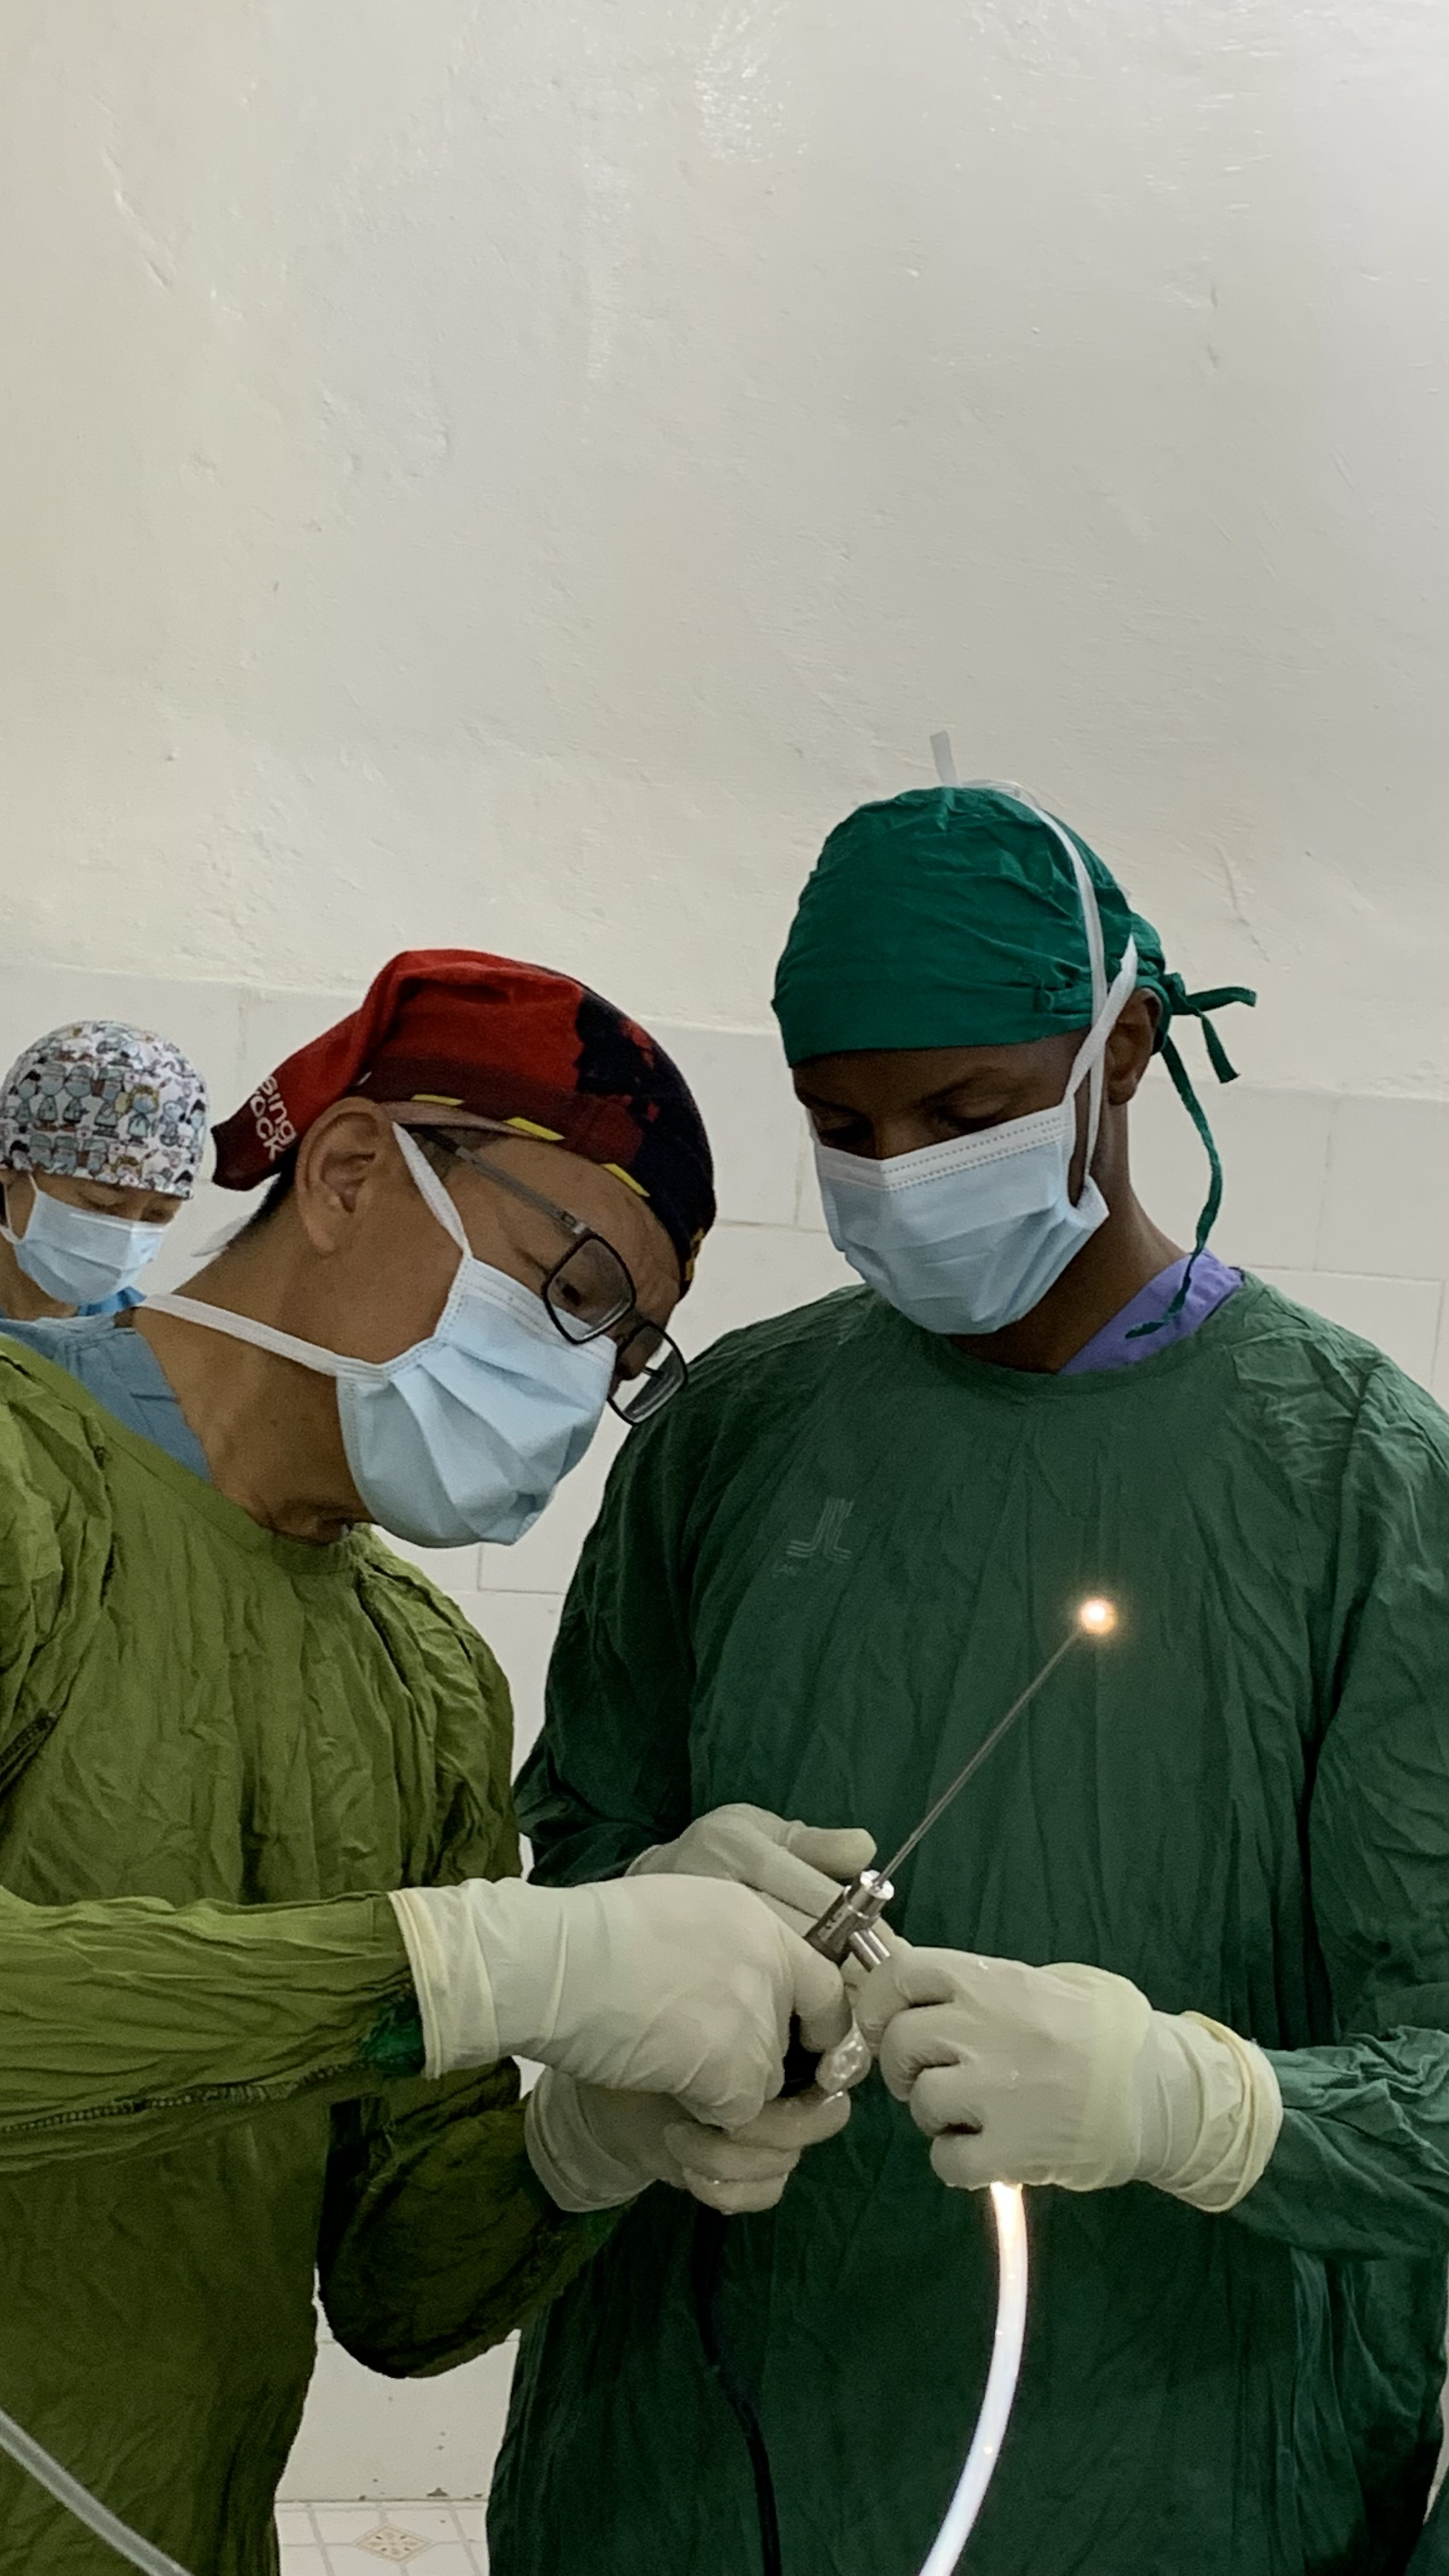
\includegraphics[width=0.30\textwidth]{IMG-6067.jpg}
        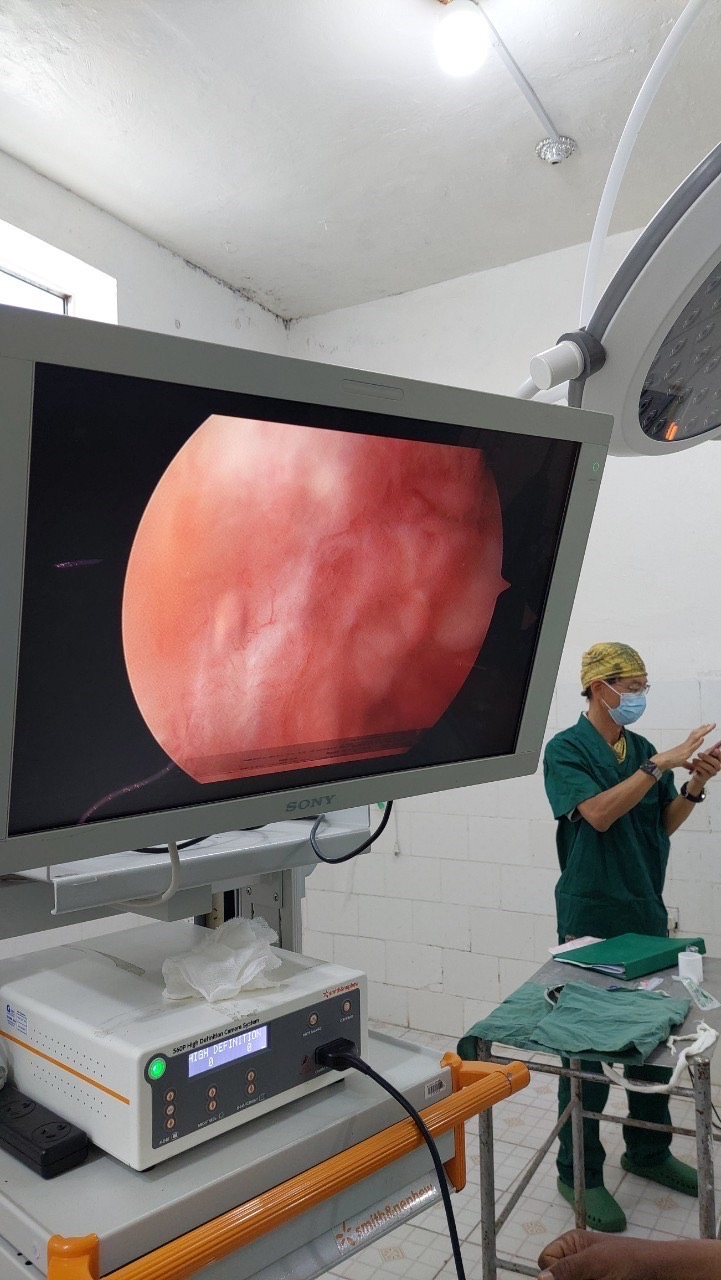
\includegraphics[width=0.30\textwidth]{IMG-6227.JPG}
    \end{center}
\end{frame}


\begin{frame}{Capacity building: nurse, urology}
    \begin{center}
        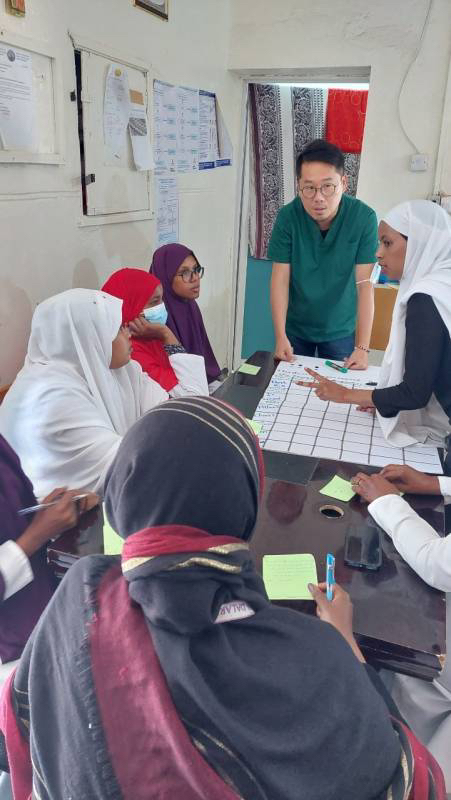
\includegraphics[width=0.30\textwidth]{6963.jpg}
        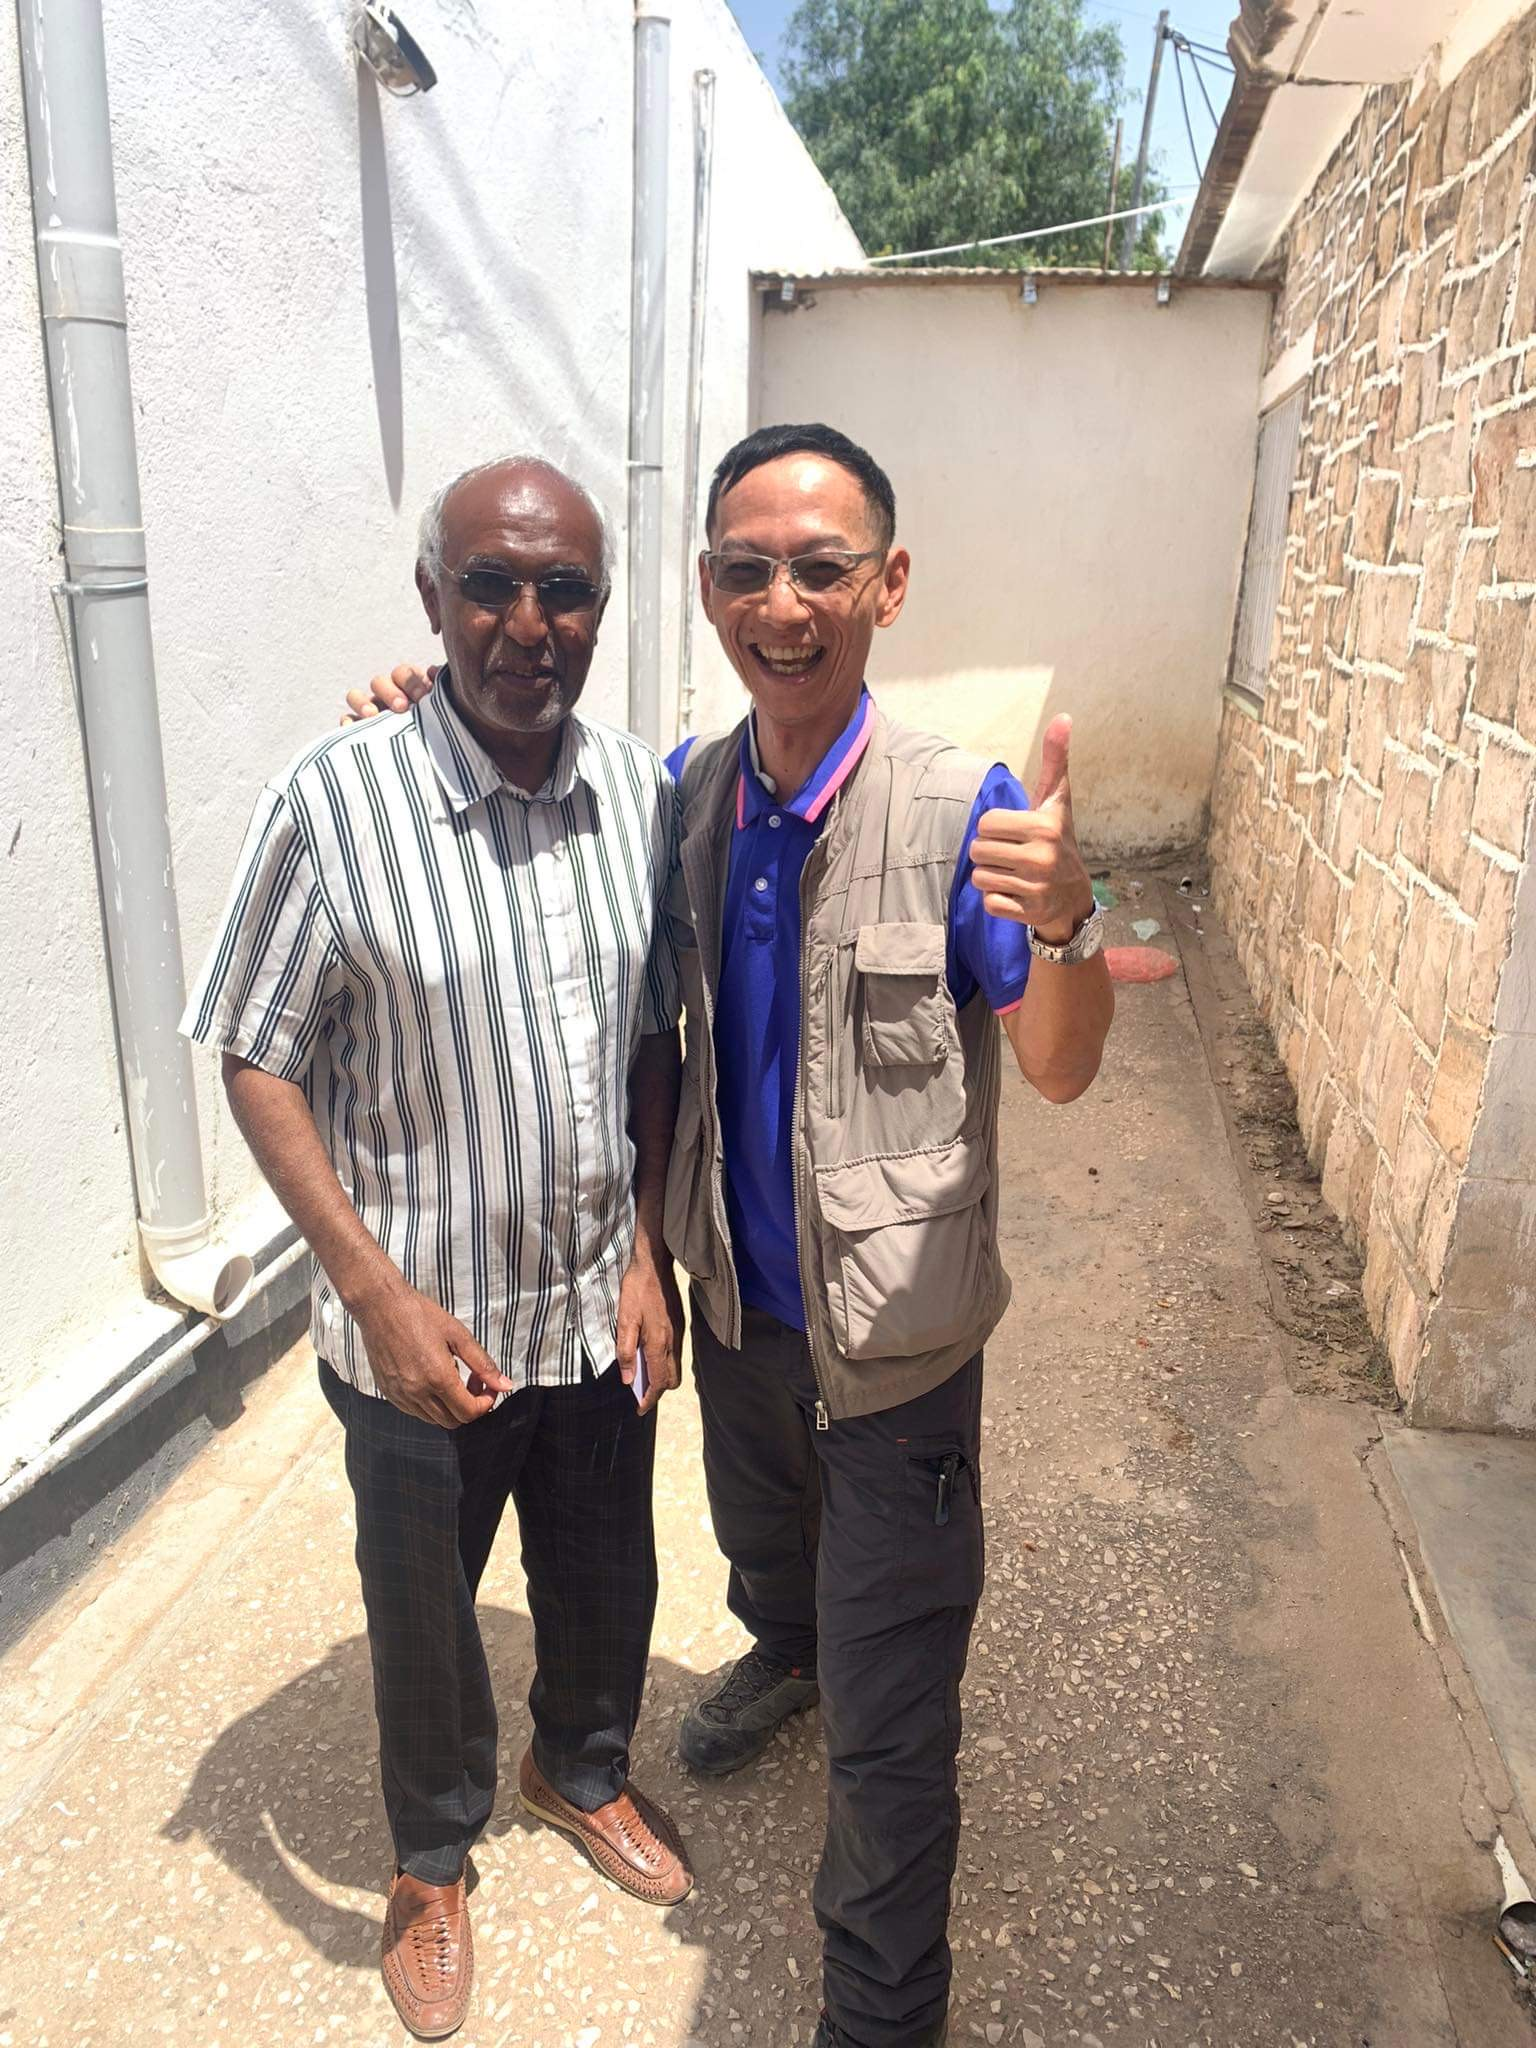
\includegraphics[width=0.30\textwidth]{IMG_5040.jpeg}
    \end{center}
\end{frame}

\begin{frame}{Nurses in TMM 醫療團的護理師}
\begin{outline}
\1 The TMM team includes a \textcolor{red}{registered nurse} (RN), working beside the obstetrician, the surgeons and the emergency doctor.
\1 \textbf{Teaching}: TMM teaches \textcolor{red}{nurses} basic skills at Hargeisa Group Hospital (HGH).
\1 \textbf{Service}: in the wards, the emergency department and on \textcolor{red}{home visits}.
\1 \textbf{Public health}: programmes that run on nursing skills ---
    \2 World Blood Donor Day (2023/06/14)
    \2 Pap smear screening for cervical cancer (since 2023/07/11)
    \2 outreach to the community (IDP site C)
\end{outline}
{\footnotesize\color{gray}教學、服務、公衛 --- 每一項都需要護理師。}
\end{frame}



\begin{frame}{Capacity building: trauma kits supplies}
    \begin{center}
        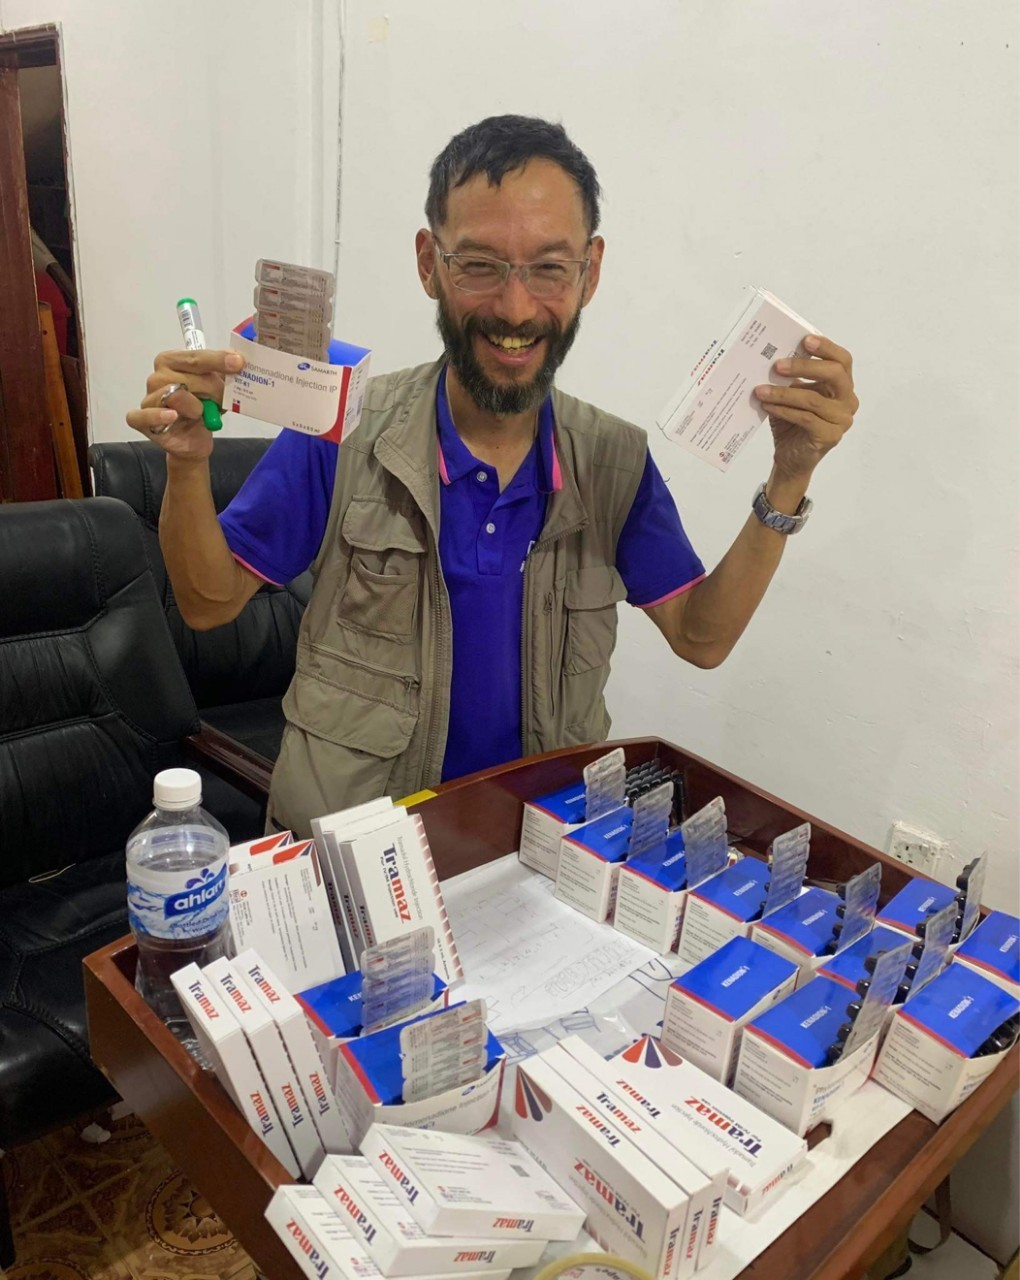
\includegraphics[width=0.33\textwidth]{4875890938550512937.32a296a9eebb4034c36c698f4a25d9d0.23050612.JPG}
        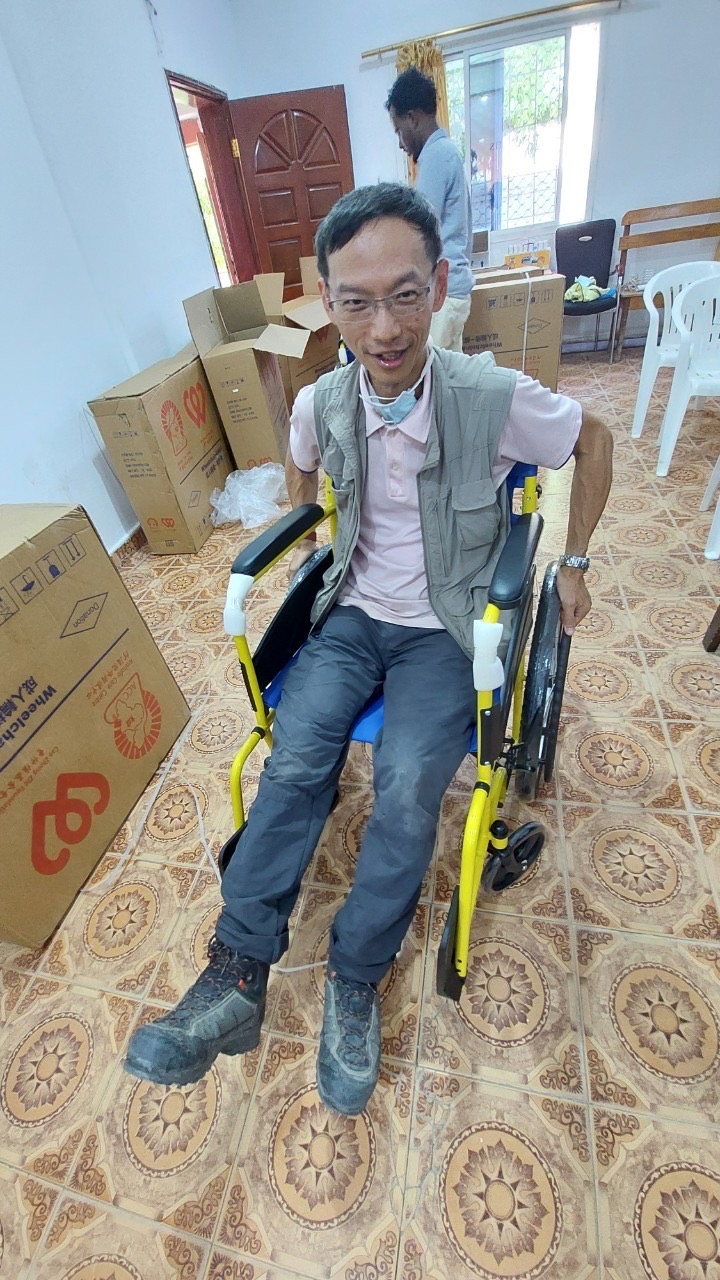
\includegraphics[width=0.30\textwidth]{IMG-2655.JPG}
        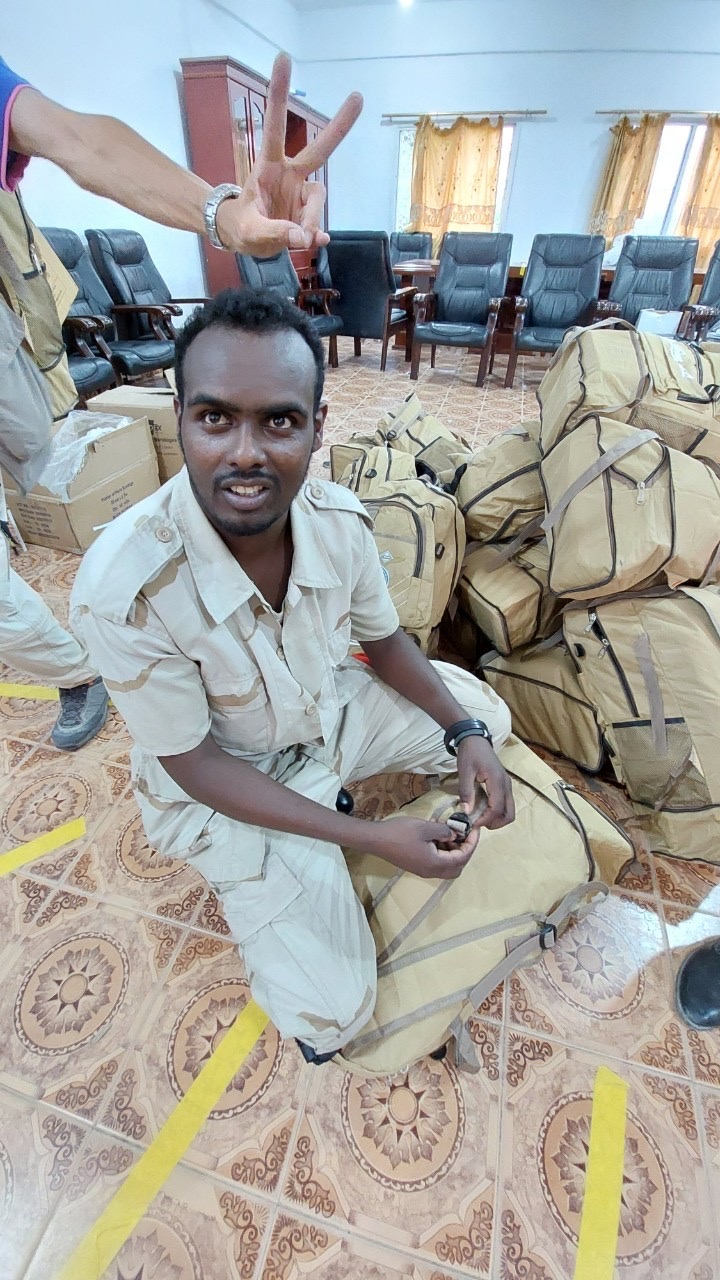
\includegraphics[width=0.30\textwidth]{IMG-2313.JPG}
%        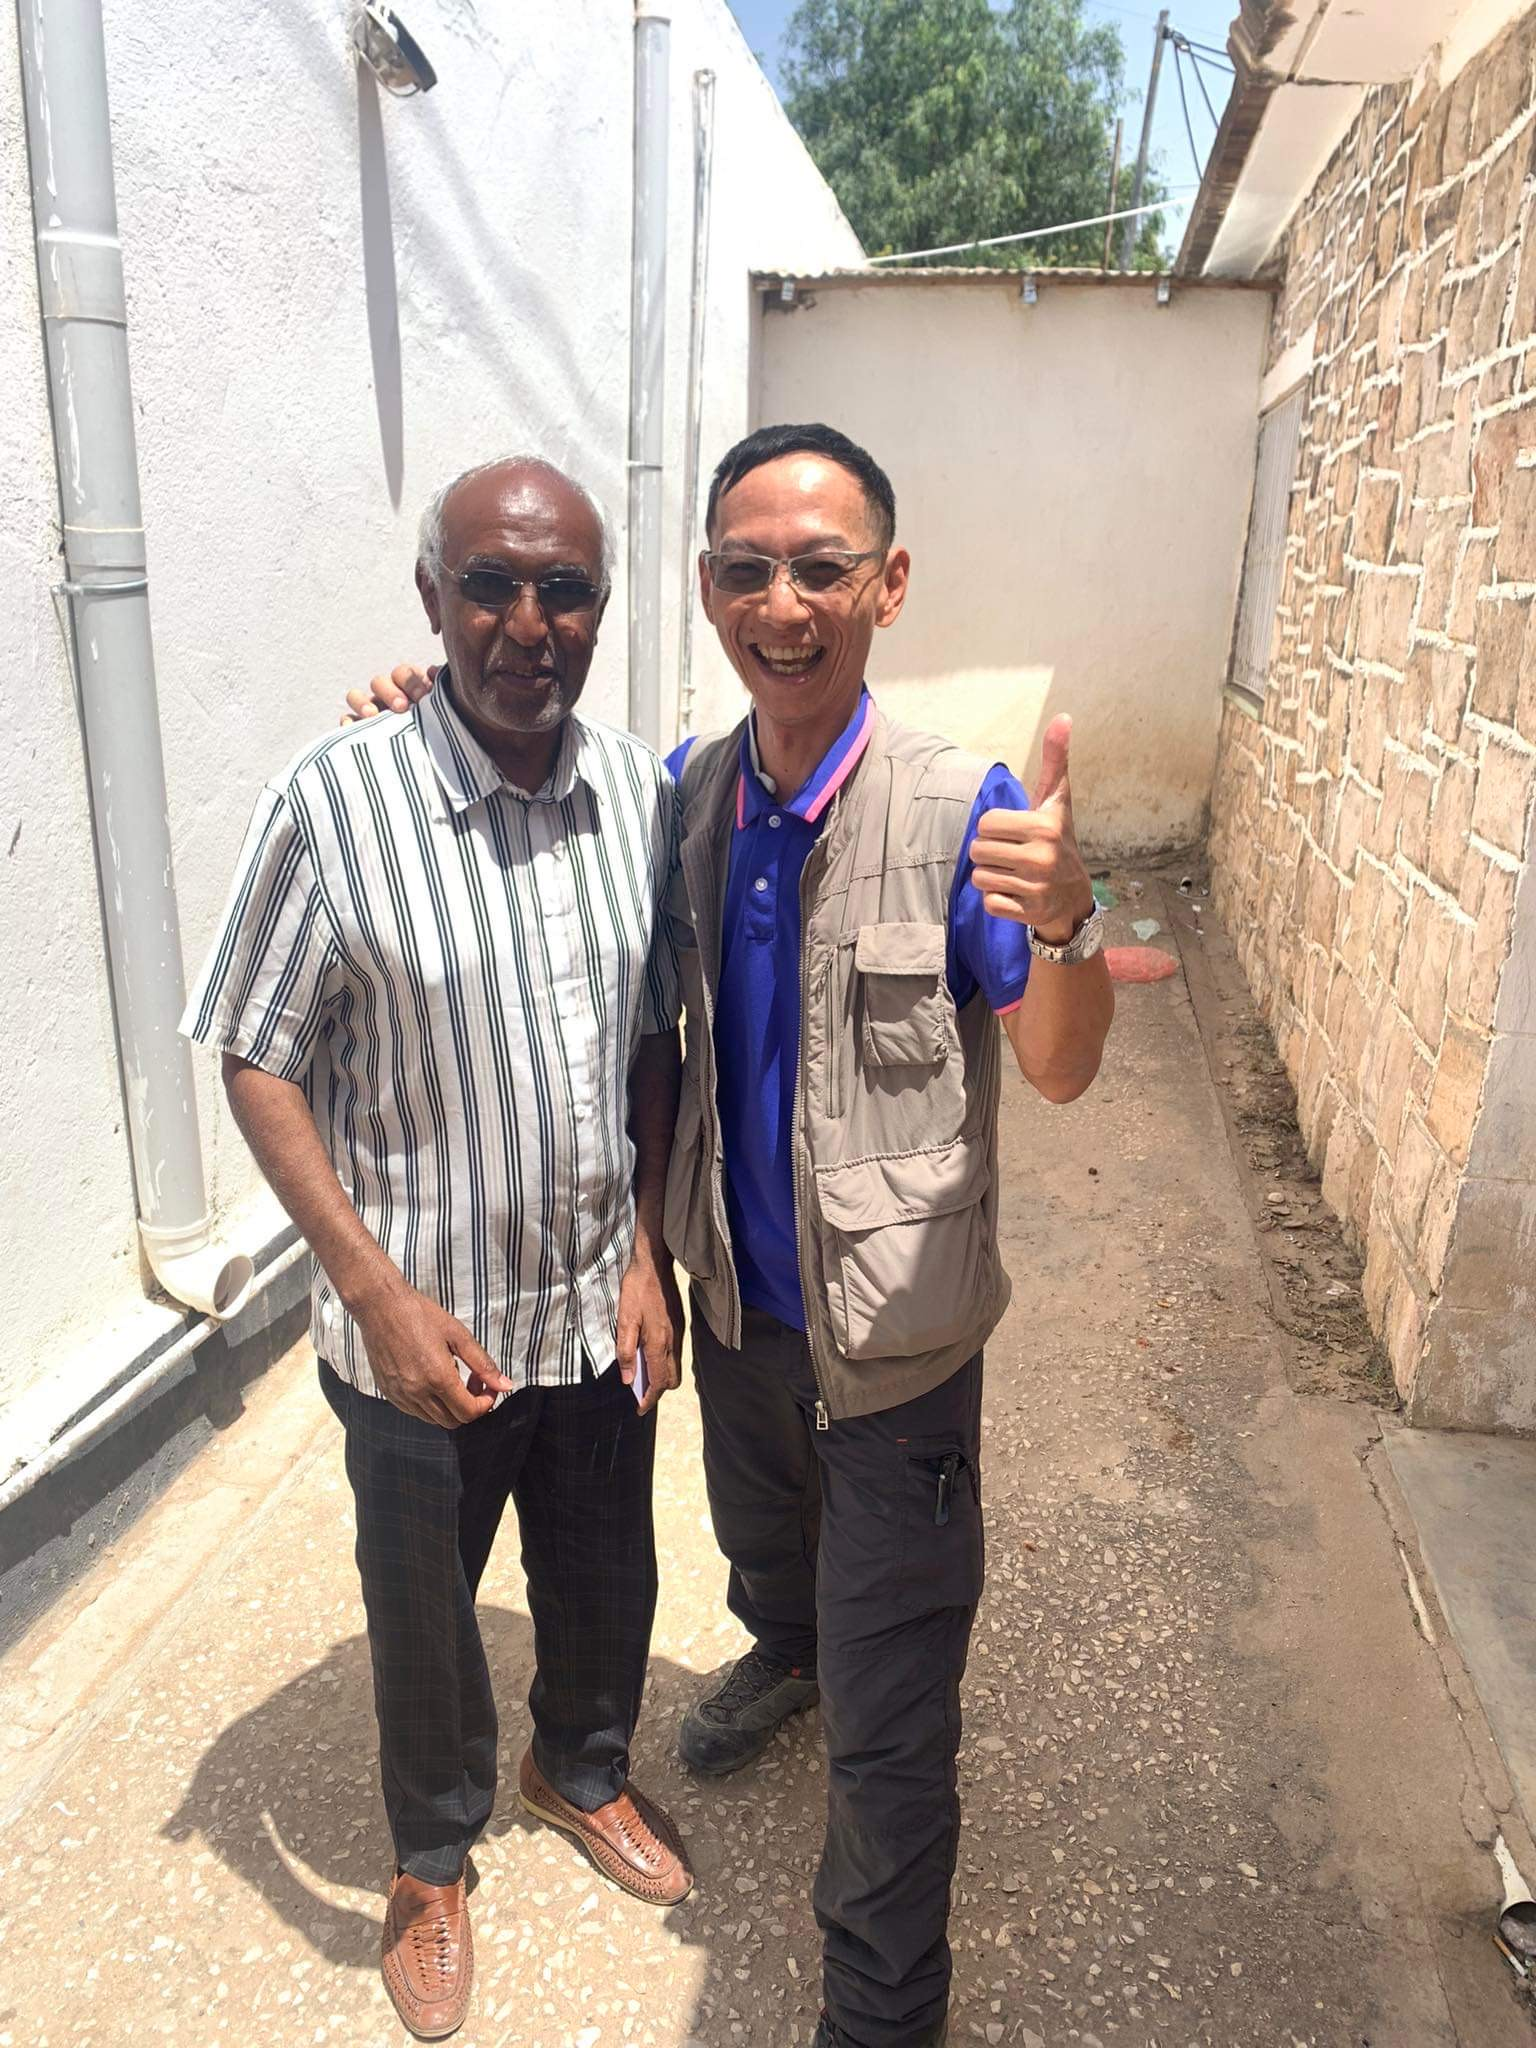
\includegraphics[width=0.24\textwidth]{IMG_5040.jpeg}    
    \end{center}
\end{frame}

\begin{frame}{Capacity building: trauma kits supplies}
    \begin{center}
        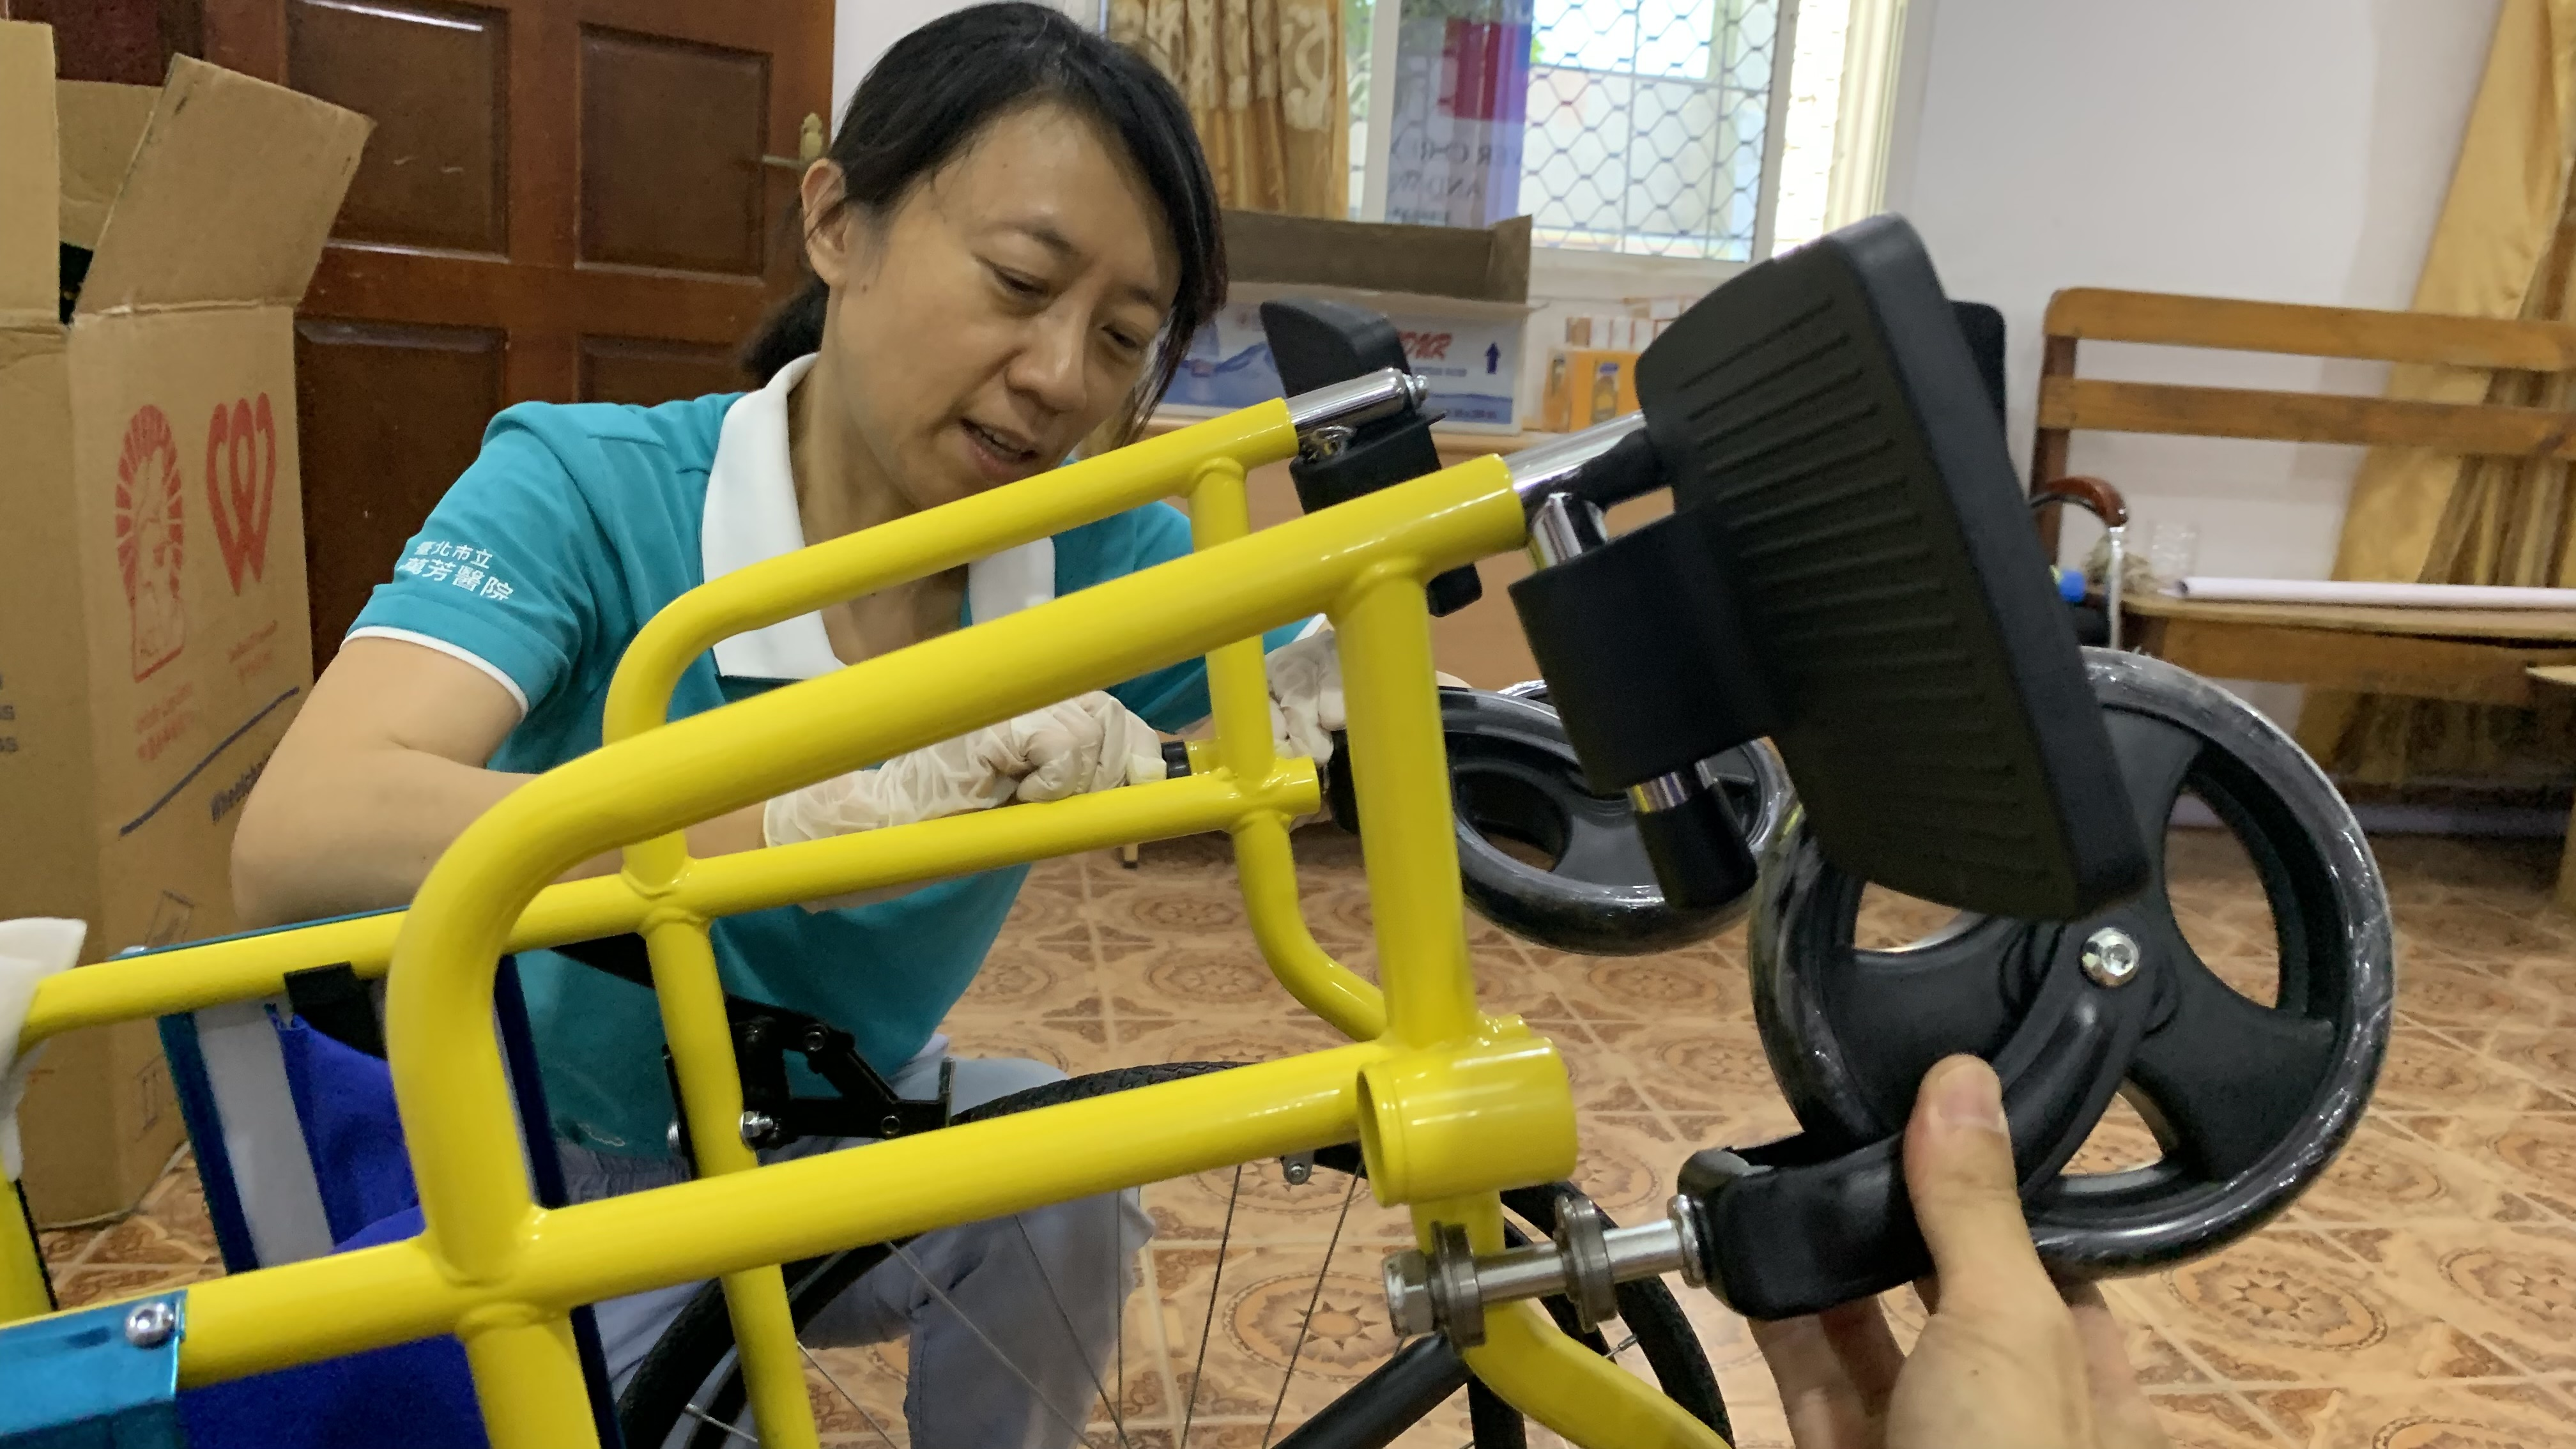
\includegraphics[width=0.4\textwidth]{IMG-2641.jpg}
        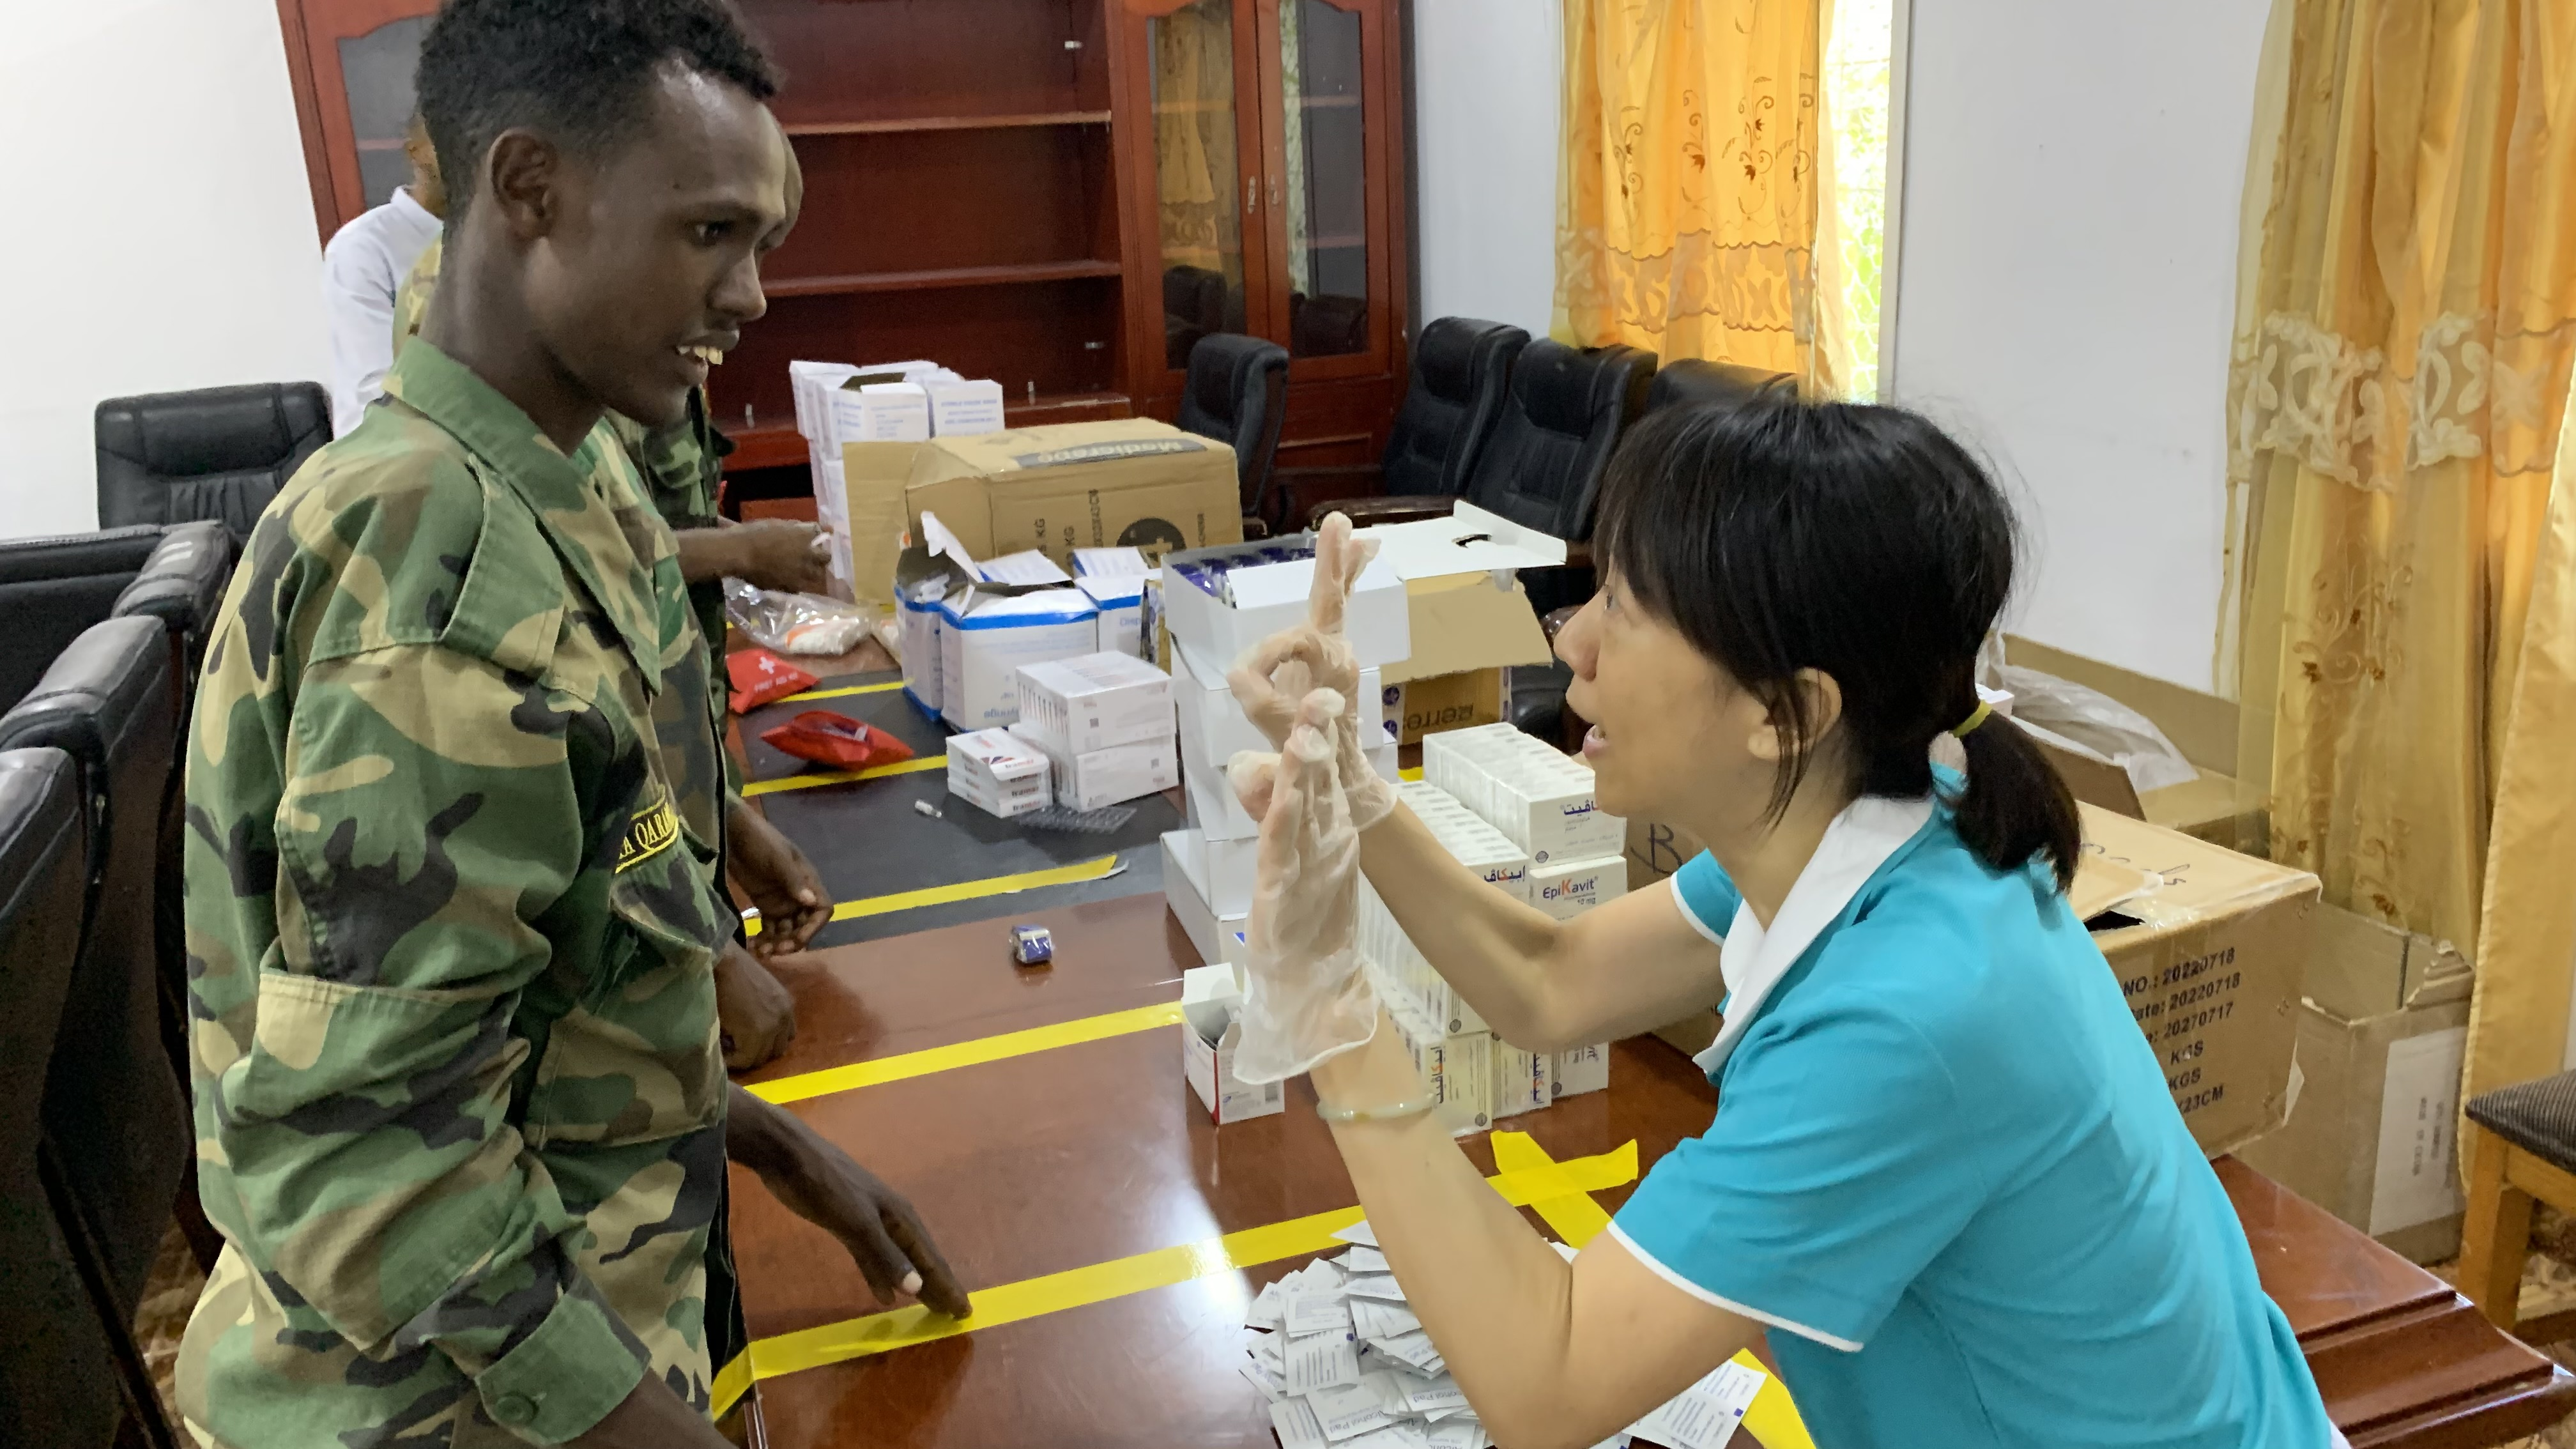
\includegraphics[width=0.4\textwidth]{IMG-2230.jpg} \\
        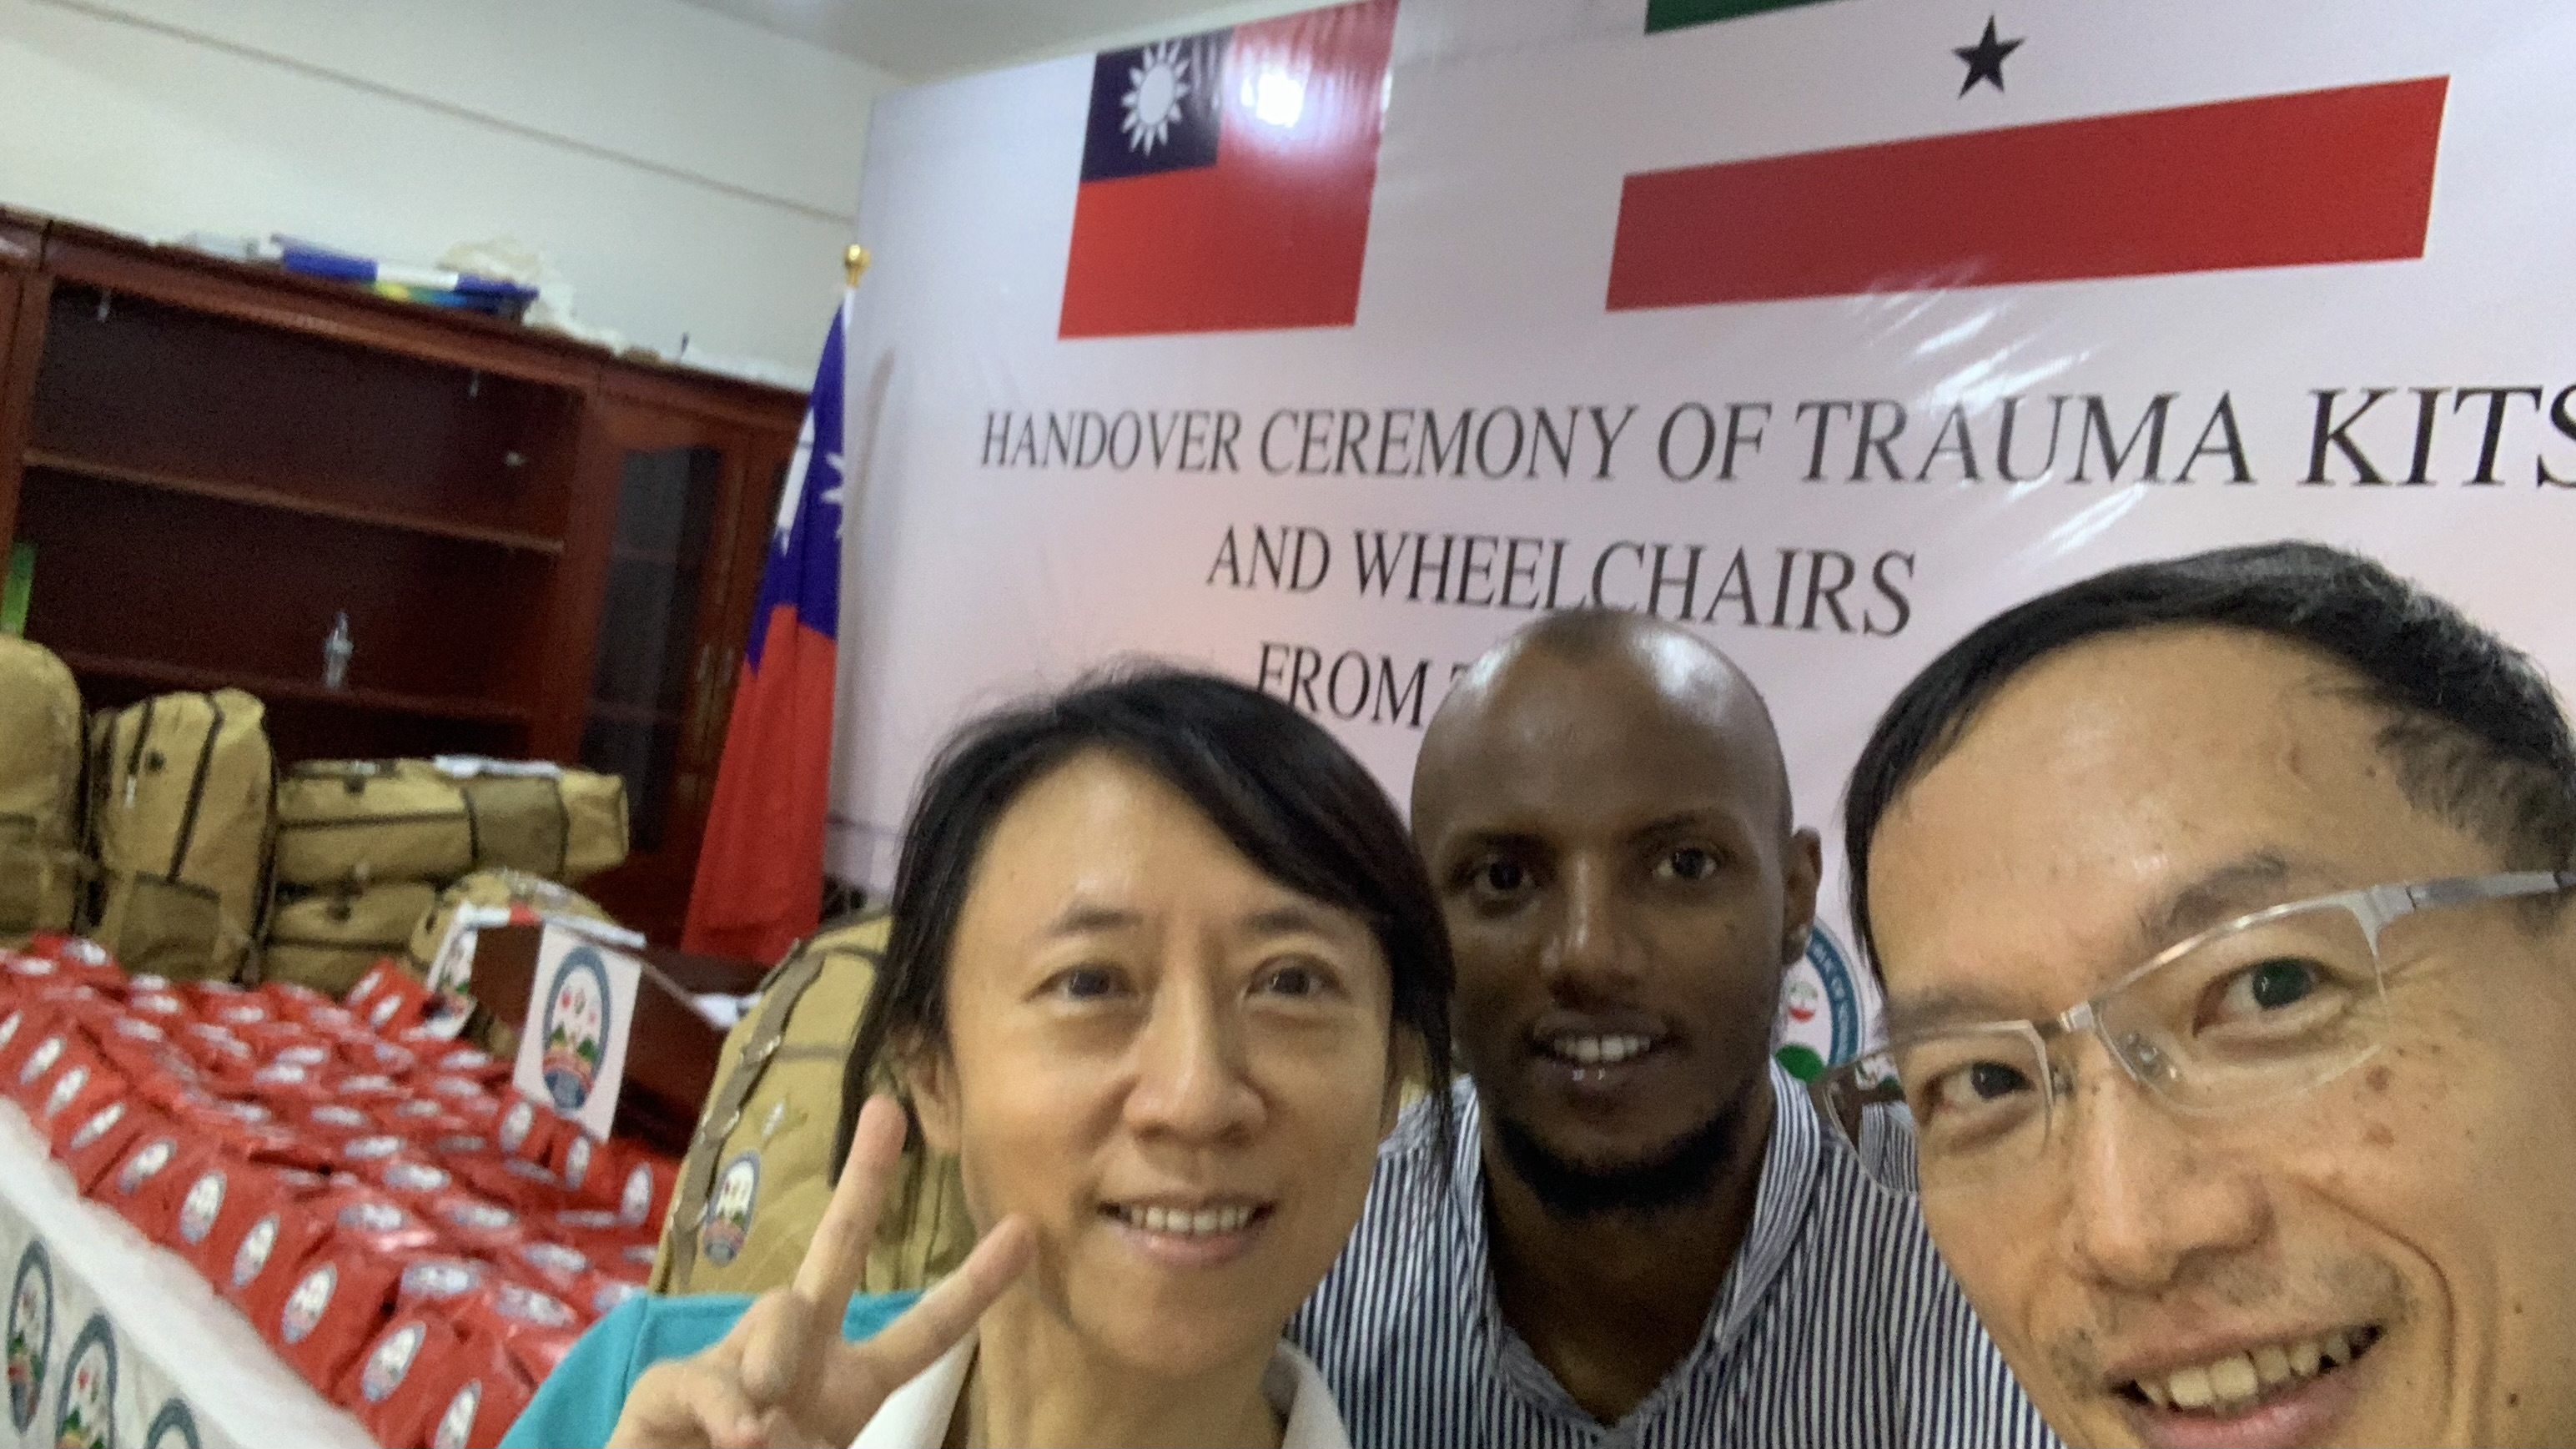
\includegraphics[width=0.4\textwidth]{IMG-2611.jpg}
        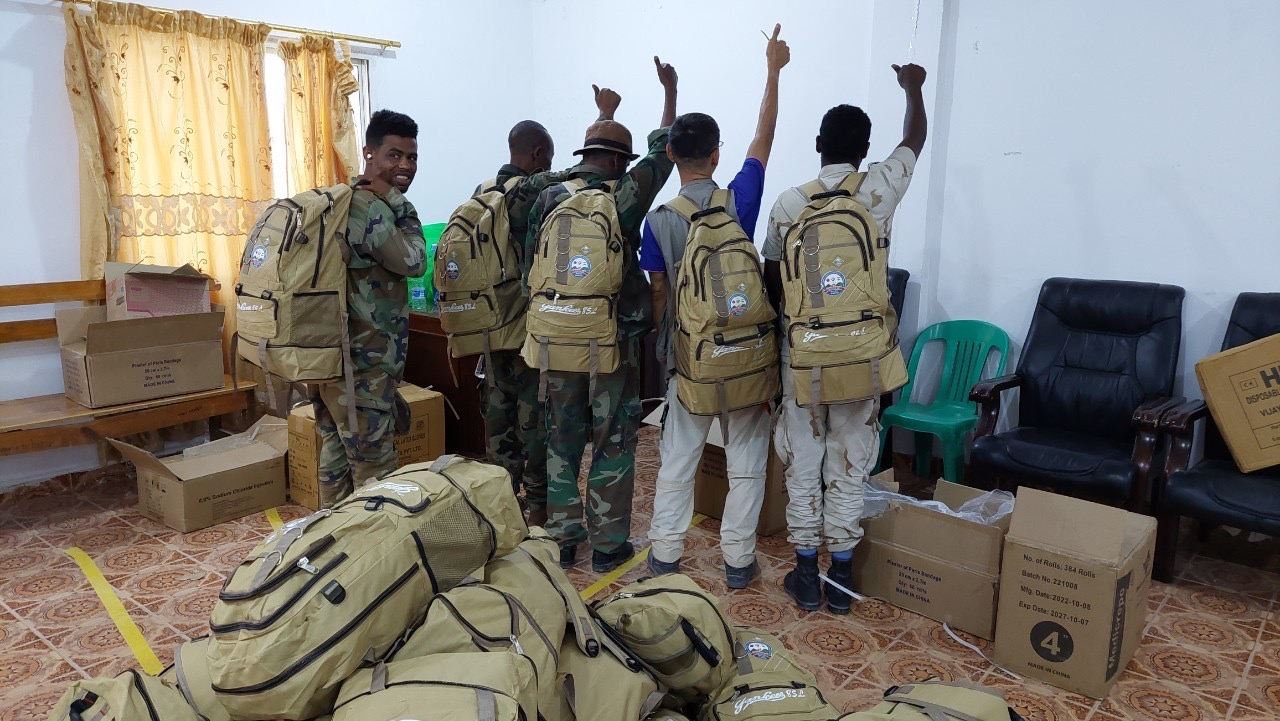
\includegraphics[width=0.4\textwidth]{IMG-2318.JPG}    
    \end{center}
\end{frame}

%%
\begin{frame}{Capacity building: trauma kits supplies}
    \begin{center}
        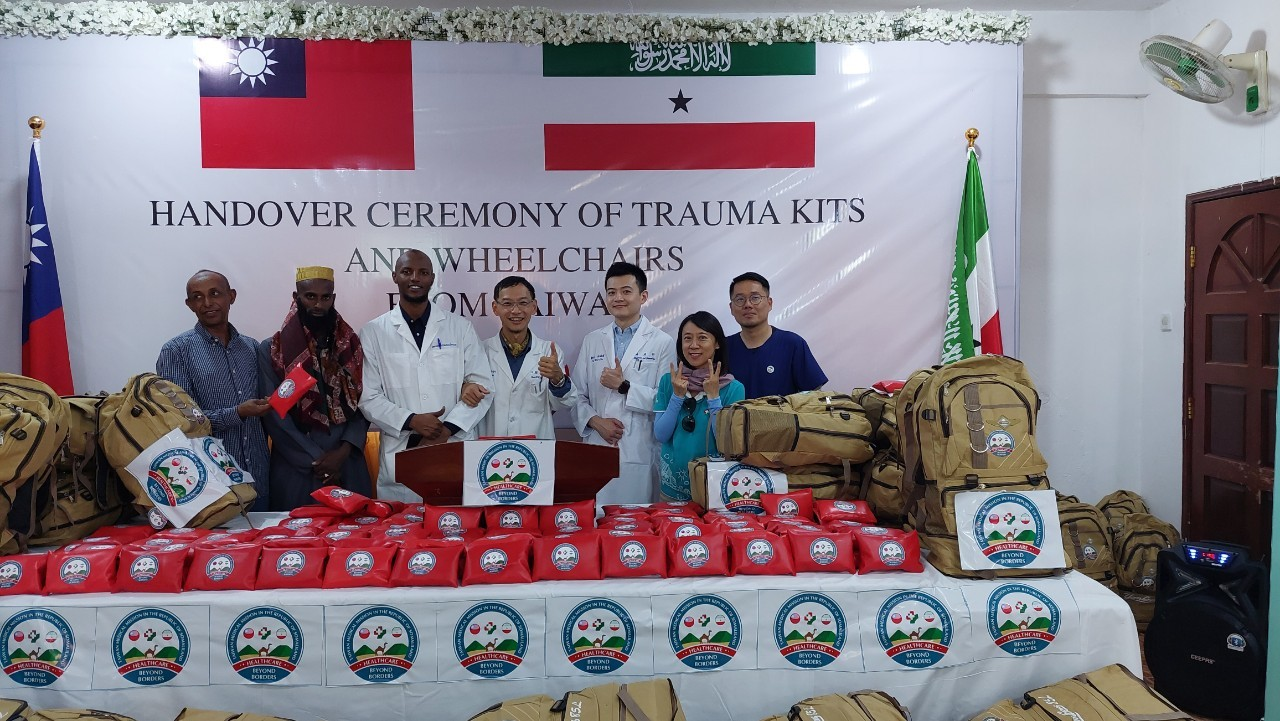
\includegraphics[width=0.8\textwidth]{4879921870343011711.12ba1a84484c21cdb54161b56f33e999.23050712.JPG}
    \end{center}
\end{frame}

%%
\begin{frame}{Field Medics — Trauma Kits in Action}
\begin{columns}[c]

\column{0.50\textwidth}
% ── TikZ: African war field, medic + yellow backpack ──
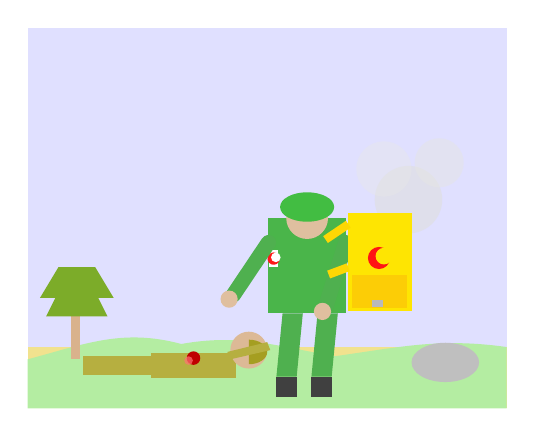
\begin{tikzpicture}[scale=0.78]
  % Sky
  \fill[blue!12!white] (0,0) rectangle (7.8,5.2);
  % Ground
  \fill[brown!45!yellow!50] (0,-1.0) rectangle (7.8,0);
  % Terrain (wavy savanna ground)
  \fill[brown!35!green!40]
    (0,-0.2) to[out=15,in=165] (2.5,0.05)
             to[out=10,in=170] (5.0,-0.15)
             to[out=8,in=172]  (7.8,0.0)
    -- (7.8,-1.0) -- (0,-1.0) -- cycle;
  % Acacia bush (left bg)
  \fill[brown!60] (0.7,-0.2) rectangle (0.85,0.5);
  \fill[green!35!brown] (0.3,0.5) -- (1.3,0.5) -- (1.0,1.1) -- (0.6,1.1) -- cycle;
  \fill[green!35!brown] (0.2,0.8) -- (1.4,0.8) -- (1.1,1.3) -- (0.5,1.3) -- cycle;
  % Rock (right bg)
  \fill[gray!50] (6.8,-0.25) ellipse (0.55 and 0.32);
  % Smoke/dust clouds (war atmosphere)
  \fill[gray!25,opacity=0.6] (6.2,2.4) circle (0.55);
  \fill[gray!20,opacity=0.5] (6.7,3.0) circle (0.40);
  \fill[gray!18,opacity=0.4] (5.8,2.9) circle (0.45);

  % ── Wounded soldier (lying, left-centre) ──
  % Legs
  \fill[olive!65] (0.9,-0.45) rectangle (2.2,-0.15);
  % Torso
  \fill[olive!65] (2.0,-0.5) rectangle (3.4,-0.1);
  % Head
  \fill[brown!55] (3.6,-0.05) circle (0.30);
  % Helmet
  \fill[olive!80] (3.6,0.12) arc(90:-90:0.30 and 0.20);
  % Wound mark
  \fill[red!75!black] (2.7,-0.18) circle (0.11);
  \fill[red!55,opacity=0.7] (2.62,-0.22) circle (0.07);
  % Outstretched arm
  \fill[olive!65] (3.3,-0.20) -- (3.95,-0.05) -- (3.90,0.08) -- (3.25,-0.08) -- cycle;

  % ── Medic (kneeling, centre-right) ──
  % Boots
  \fill[black!75] (4.05,-0.82) rectangle (4.38,-0.48);
  \fill[black!75] (4.62,-0.82) rectangle (4.95,-0.48);
  % Legs
  \fill[green!38!gray] (4.05,-0.48) -- (4.38,-0.48) -- (4.48,0.55) -- (4.15,0.55) -- cycle;
  \fill[green!38!gray] (4.62,-0.48) -- (4.95,-0.48) -- (5.05,0.55) -- (4.72,0.55) -- cycle;
  % Torso
  \fill[green!42!gray] (3.92,0.55) rectangle (5.18,2.10);
  % Head
  \fill[brown!50] (4.55,2.10) circle (0.34);
  % Helmet
  \fill[green!48!gray] (4.55,2.28) ellipse (0.44 and 0.24);
  % Red Crescent armband (Islamic humanitarian symbol)
  \fill[white] (3.93,1.30) rectangle (4.08,1.58);
  \fill[red!90] (4.005,1.44) circle (0.10);
  \fill[white] (4.040,1.46) circle (0.078);
  % Arms reaching toward wounded
  \draw[green!38!gray,line width=5.5pt,line cap=round] (3.92,1.70) -- (3.35,0.85);
  \draw[green!38!gray,line width=5.5pt,line cap=round] (5.18,1.70) -- (4.85,0.65);
  \fill[brown!50] (3.28,0.78) circle (0.14);
  \fill[brown!50] (4.80,0.58) circle (0.14);

  % ── BIG YELLOW BACKPACK ──
  \fill[yellow!88!orange] (5.22,0.58) rectangle (6.25,2.18);
  % Front pocket
  \fill[yellow!65!orange] (5.28,0.64) rectangle (6.18,1.18);
  % Shoulder straps
  \draw[yellow!75!orange,line width=3pt] (5.22,2.00) -- (4.85,1.75);
  \draw[yellow!75!orange,line width=3pt] (5.22,1.30) -- (4.90,1.18);
  % RED CRESCENT (prominent — Islamic humanitarian symbol)
  \fill[red!92] (5.72,1.45) circle (0.18);
  \fill[yellow!88!orange] (5.80,1.48) circle (0.135);
  % Buckle
  \fill[gray!55] (5.60,0.65) rectangle (5.78,0.76);
\end{tikzpicture}

\column{0.50\textwidth}
\begin{outline}
\1 \textbf{TMM builds trauma kits for\\Somaliland Armed Forces}
  \2 Custom yellow field backpacks\\(marked with Red Crescent \redcrescent)
  \2 Tourniquet, haemostatic gauze,\\chest seal, bandages
\1 \textbf{Field training}
  \2 TMM medics train local military\\medical officers on-site
  \2 Working \textcolor{red}{side-by-side}\\as equal partners
\1 \textcolor{red}{``Save the first hour''} —\\combat casualty care
\end{outline}
\end{columns}
\end{frame}

\begin{frame}{Capacity building: others}
    \begin{center}
        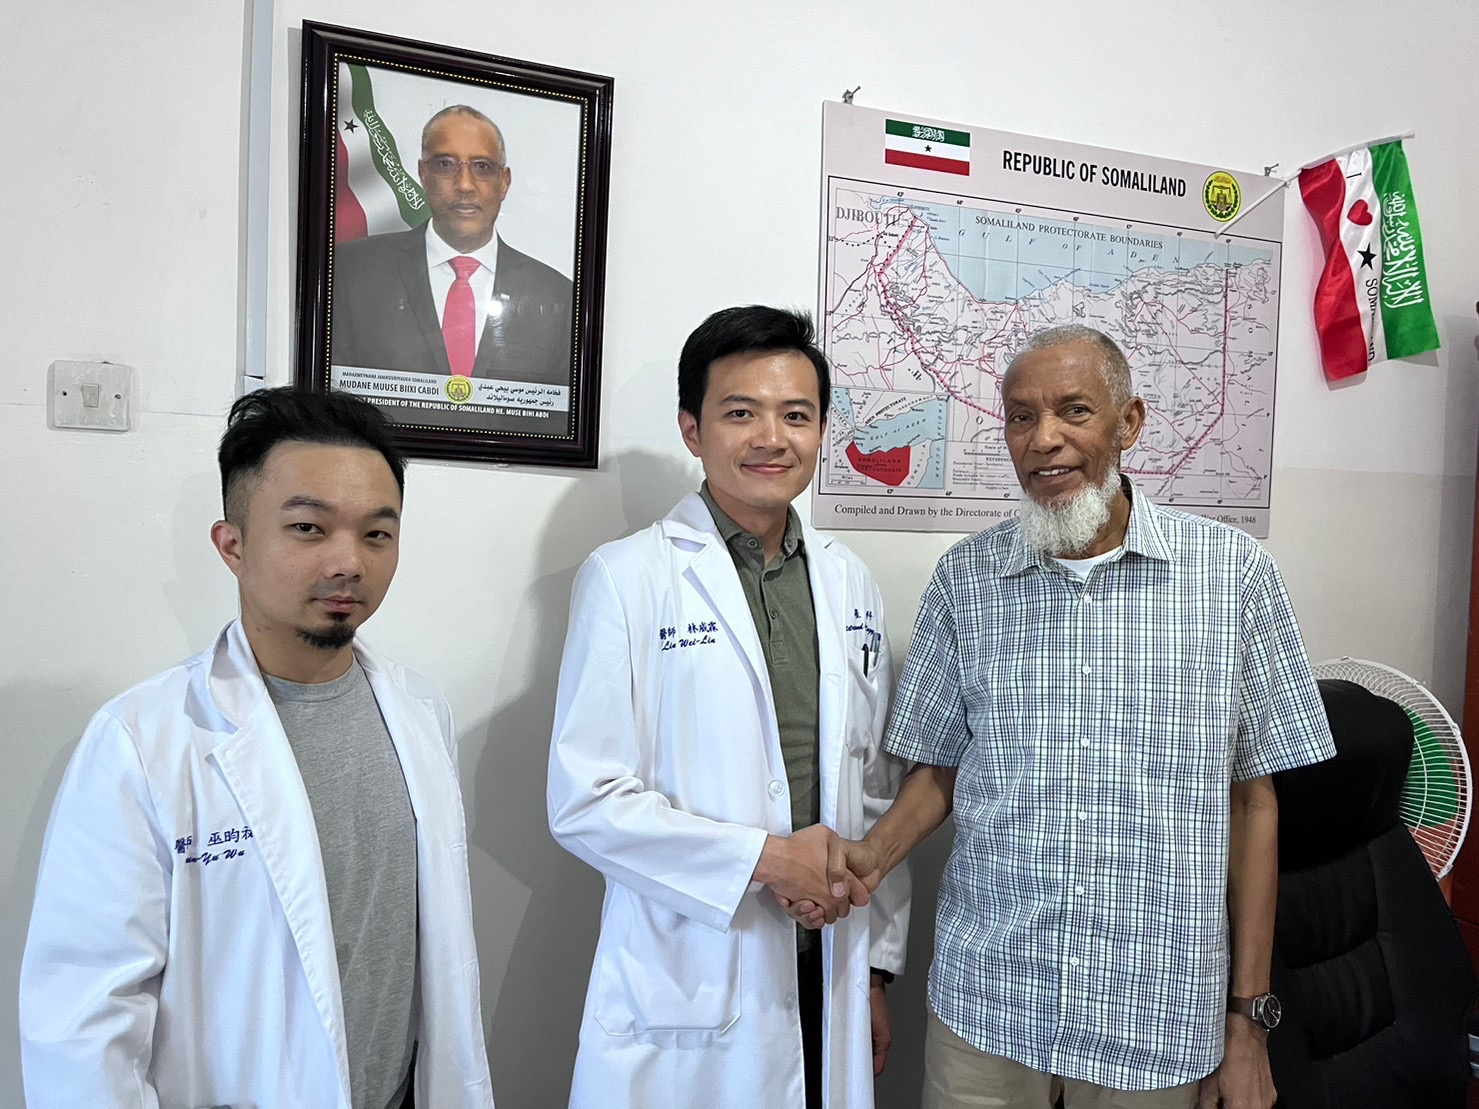
\includegraphics[width=0.24\textwidth]{IMG-5107.JPG}
        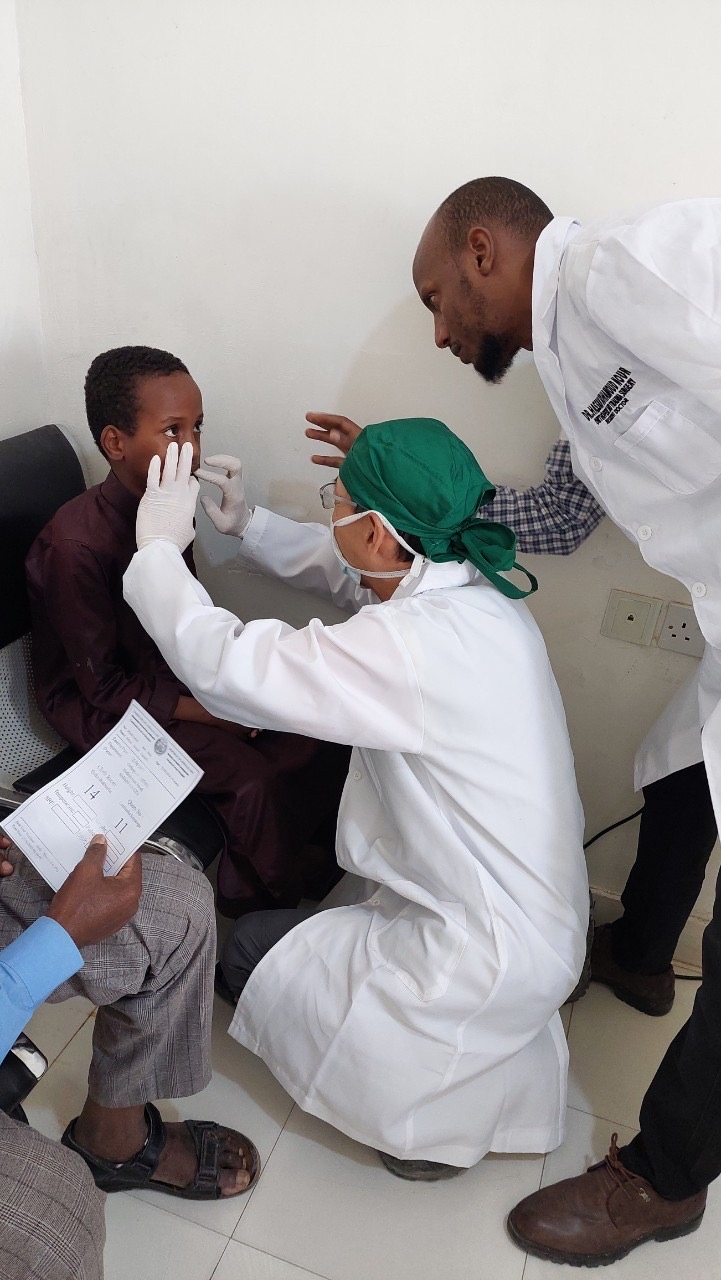
\includegraphics[width=0.24\textwidth]{IMG-4703.JPG}
        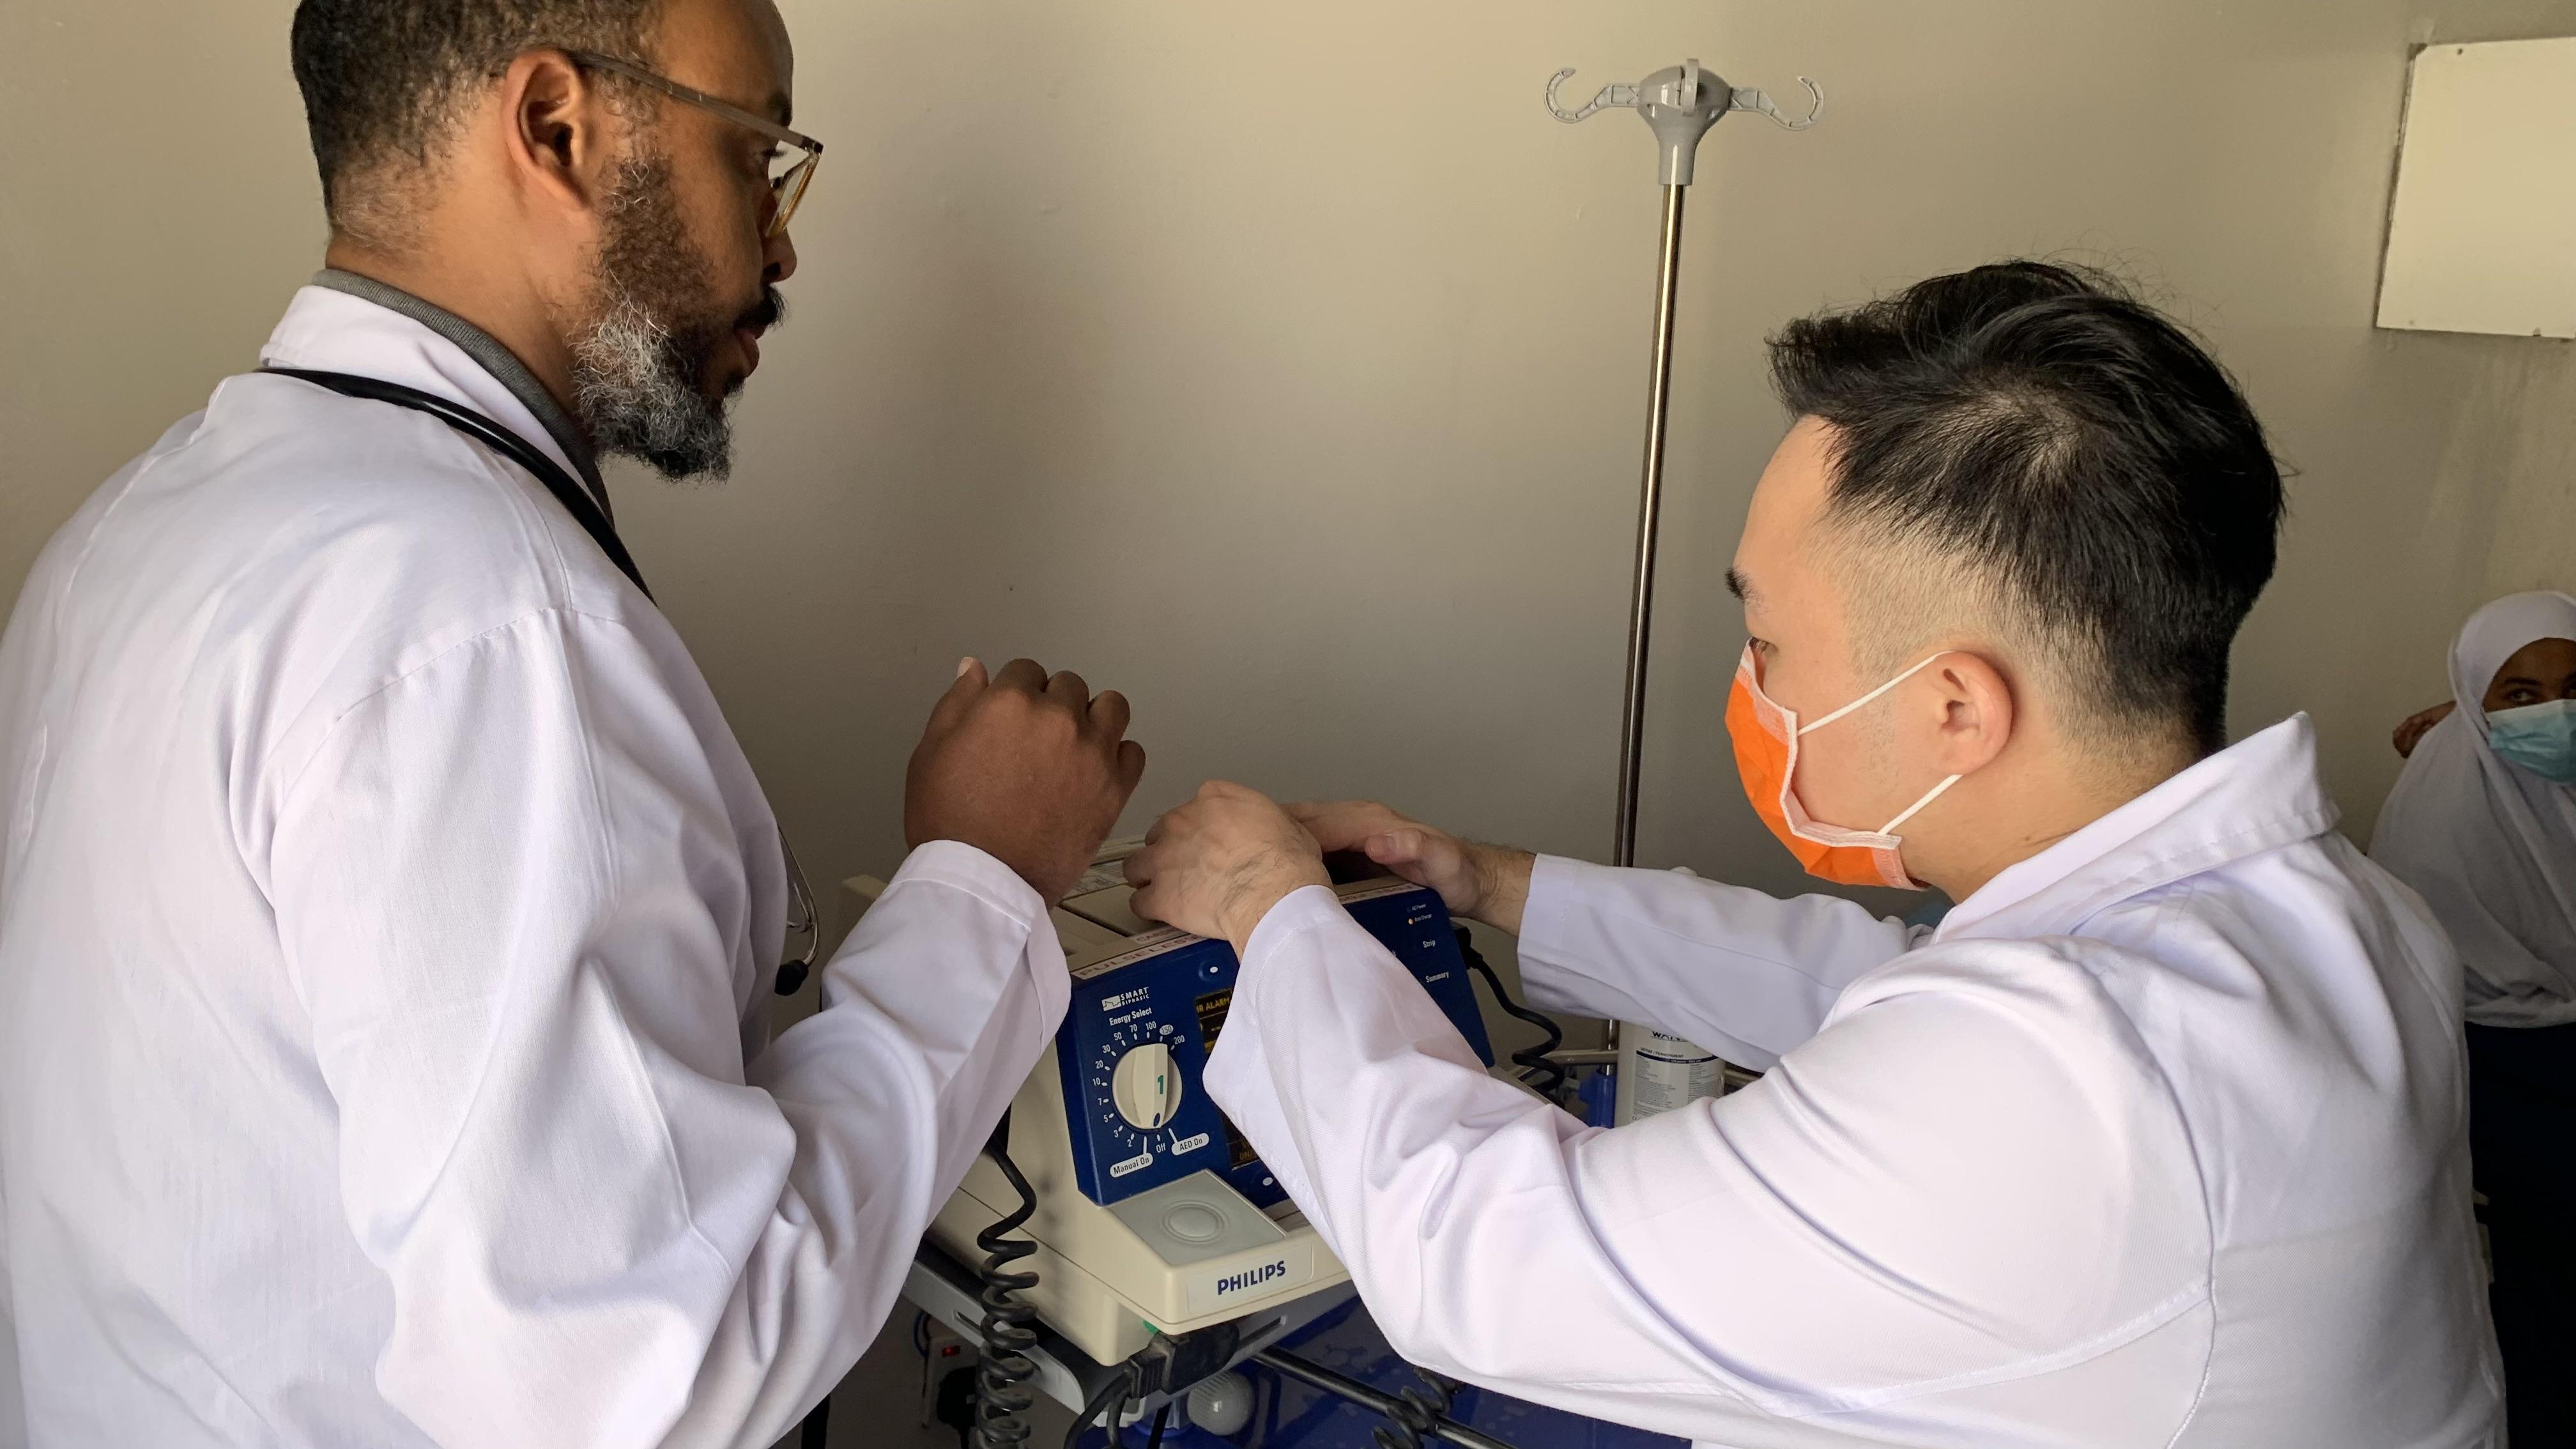
\includegraphics[width=0.24\textwidth]{IMG-5062.JPG}
        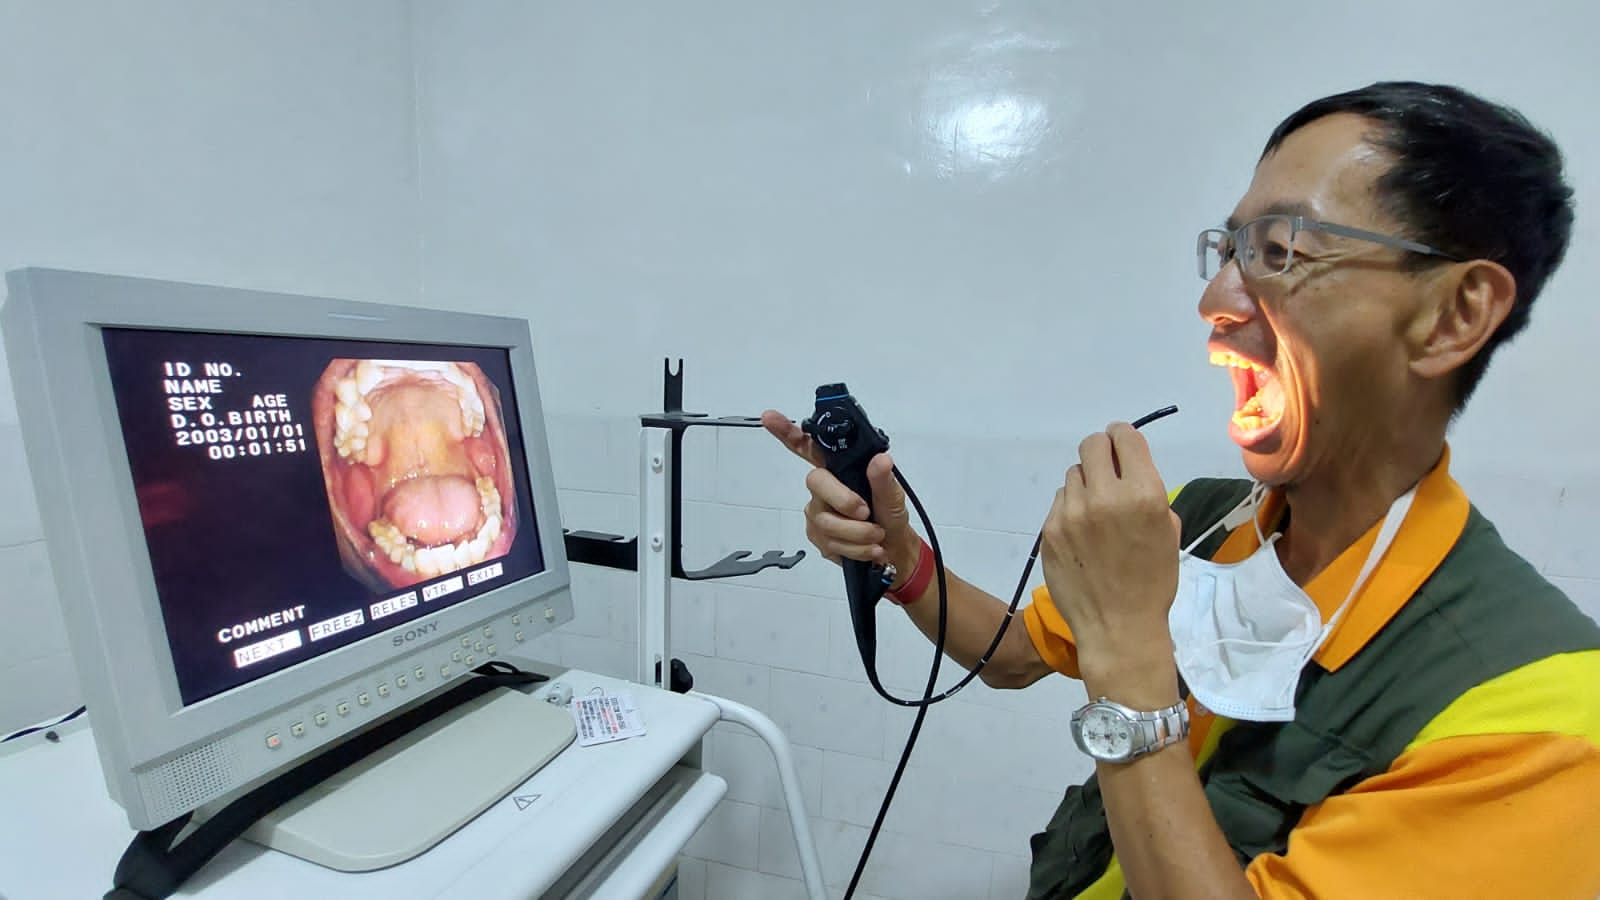
\includegraphics[width=0.24\textwidth]{6a625355-ae53-4e8f-891e-38a933f6c29b.JPG}    
    \end{center}
\end{frame}
%%    
\begin{frame}
\frametitle{TMM's Projects - third pillar}
% Add content here
\begin{outline}    
    \1 public health, we are launching
        \2 World Blood Donor Day campaign (2023/06/14)
        \2 Pap smear screen for elimination of cervical cancer (since 2023/07/11)
        \2 Good oral hygiene and oral cancer screening (March 2024)
        \2 HBV/HCV screenings, vaccinations, and treatment (2025)
        \2 Osteoprosis screening for women who get vitamin D deficience (Nov 2024)
        \2 Parasite screening program for schoolchildren (2025)
\end{outline}

\begin{center}
\includesvg[width=0.14\textwidth]{Blood_logo.svg}
\includesvg[width=0.14\textwidth]{anti_CervicalCancer_logo.svg}
\includesvg[width=0.22\textwidth]{World_OralHealth_Day_logo.svg}
\includesvg[width=0.14\textwidth]{WHD_logo.svg}
\includesvg[width=0.2\textwidth]{parasite_logo.svg}
\end{center}

\end{frame}

%%%

\begin{frame}{Oral health research}
\begin{outline}

Public health, we are studying
    \1 Exploring the Prevalence of \textcolor{red}{Halitosis and Tonsillitis} in Hargeisa Group Hospital, Somaliland: A Retrospective Pilot Study
        \2 Dr. Fadumo, Dr. Hersi, Dr. Omar, and Dr. Tex
    \1 Evaluating the Diagnostic Accuracy of CT-Scans and Serum Fluoride Levels in Detecting \textcolor{red}{Skeletal Fluorosis} in the Somaliland Population with \textcolor{red}{Dental Fluorosis}
        \2 Dr. Mukhtar, Dr. Fadumo, Dr. Ahmed Hashi, and Dr. Tex
    \1 (TOM) AI-assistant Osteoporosis diagnosis
        \2 AI can tell \textcolor{red}{bone density} from a pelvic X-ray
\end{outline}
    
\end{frame}


%%
\begin{frame}{Public health: Oral health}
    \begin{columns}
        
    \column{0.5\textwidth}
        \begin{center}
        \includesvg[width=0.7\textwidth]{World_OralHealth_Day_logo.svg}
            
        \end{center}
    \column{0.5\textwidth}
        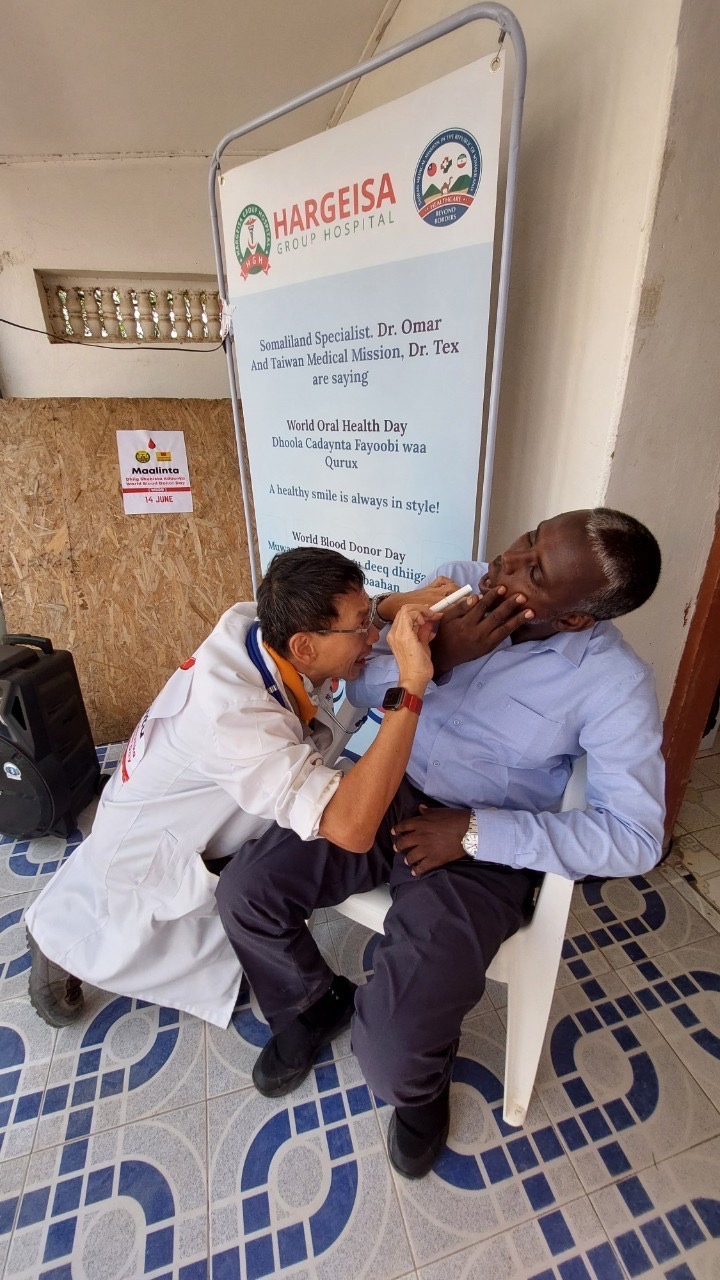
\includegraphics[width=0.7\textwidth]{IMG-4368.JPG}
%        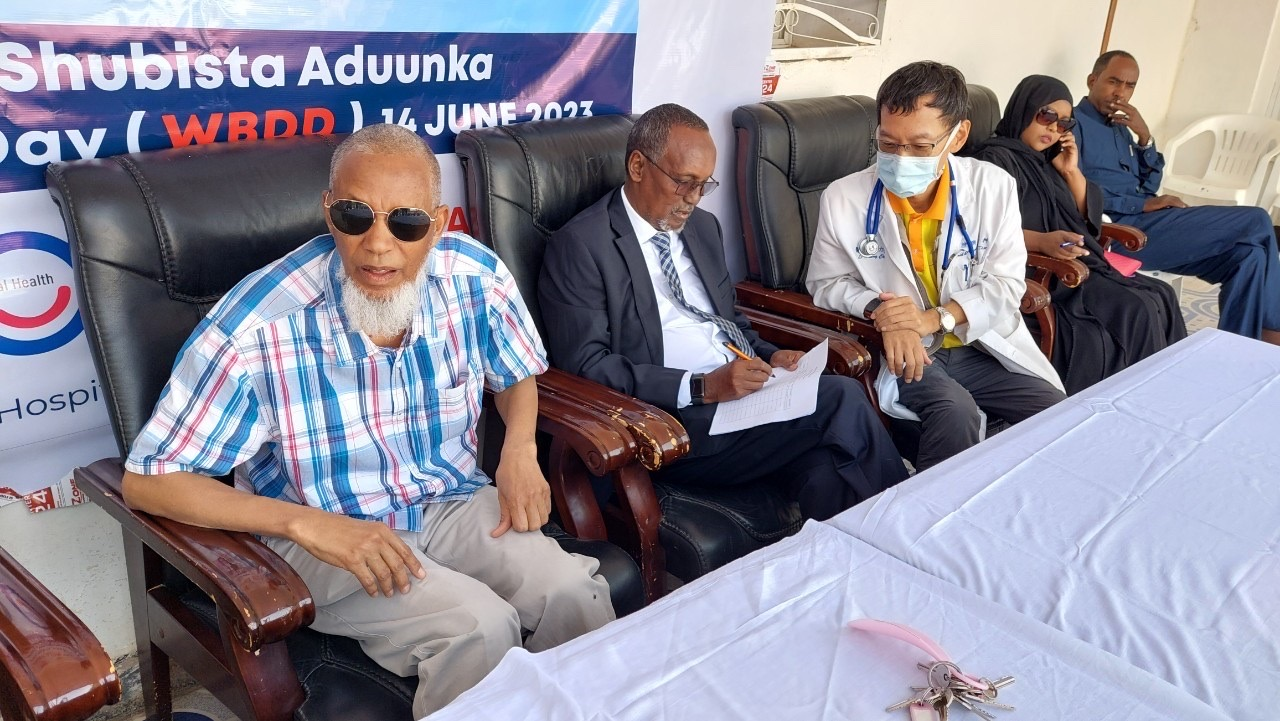
\includegraphics[width=0.45\textwidth]{IMG-4378.JPG}
    \end{columns}
\end{frame}




% Dr Askar
\begin{frame}{Public health: World Blood Donor Day}
    \begin{center}
        \includesvg[width=0.2\textwidth]{Blood_logo.svg}
%        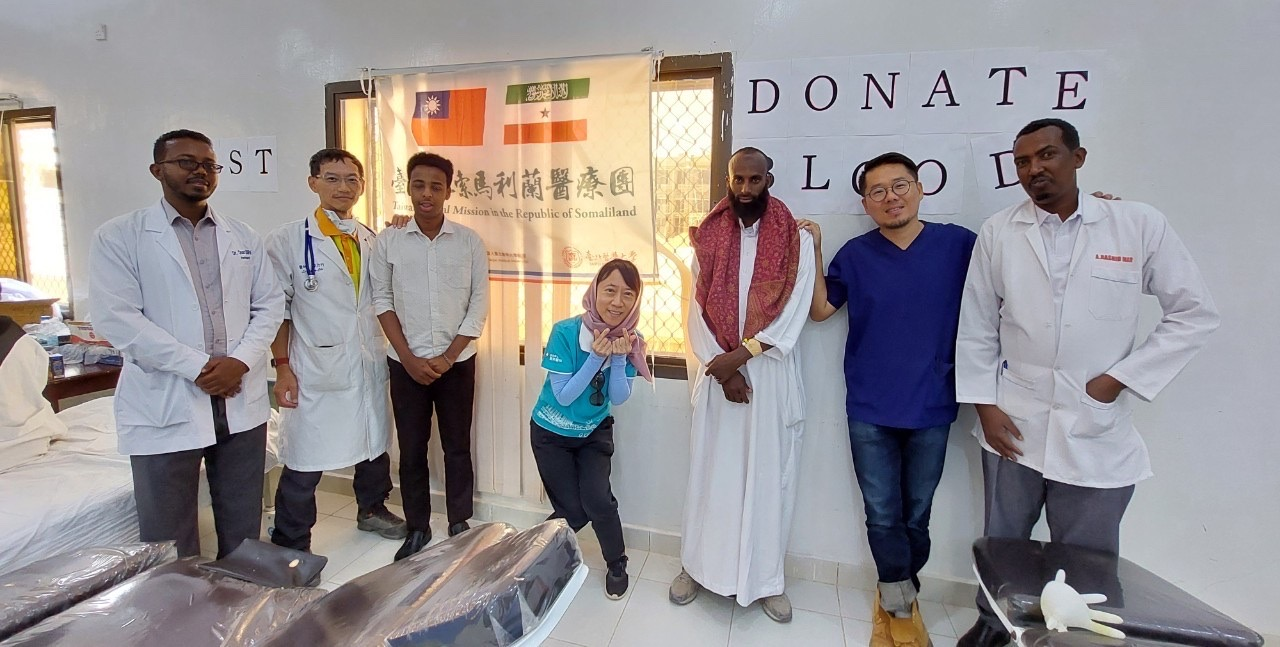
\includegraphics[width=0.35\textwidth]{IMG-4441.JPG}
        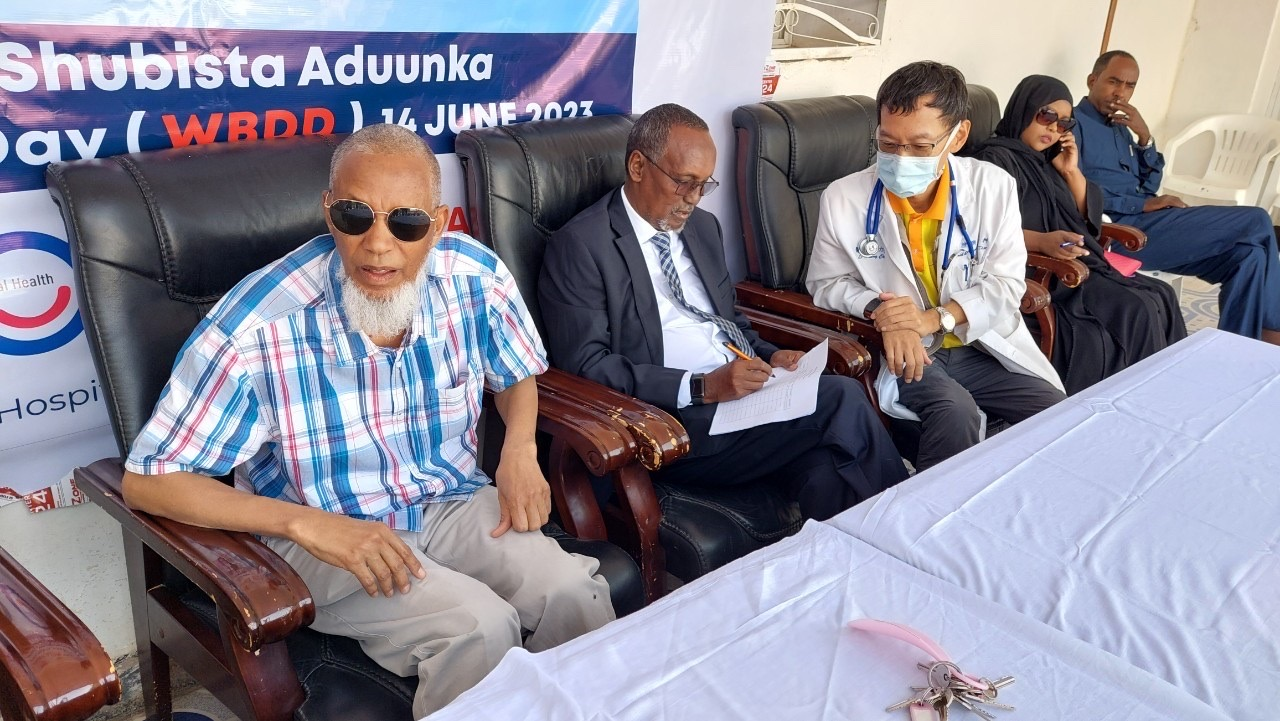
\includegraphics[width=0.75\textwidth]{IMG-4378.JPG}
    \end{center}
\end{frame}

% UoH student
\begin{frame}{Public health: World Blood Donor Day}
    \begin{center}
        \includesvg[width=0.2\textwidth]{Blood_logo.svg}
        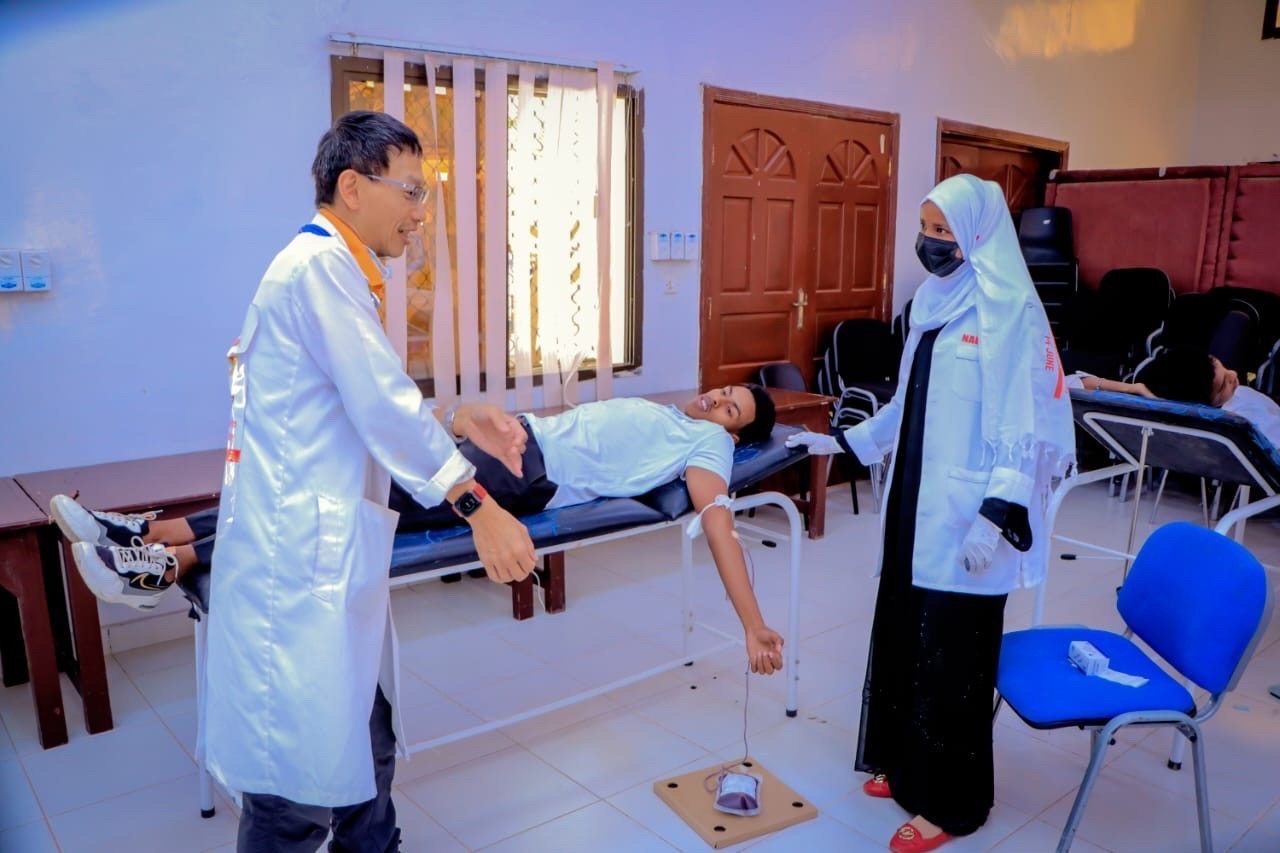
\includegraphics[width=0.45\textwidth]{IMG-5110.JPG}
        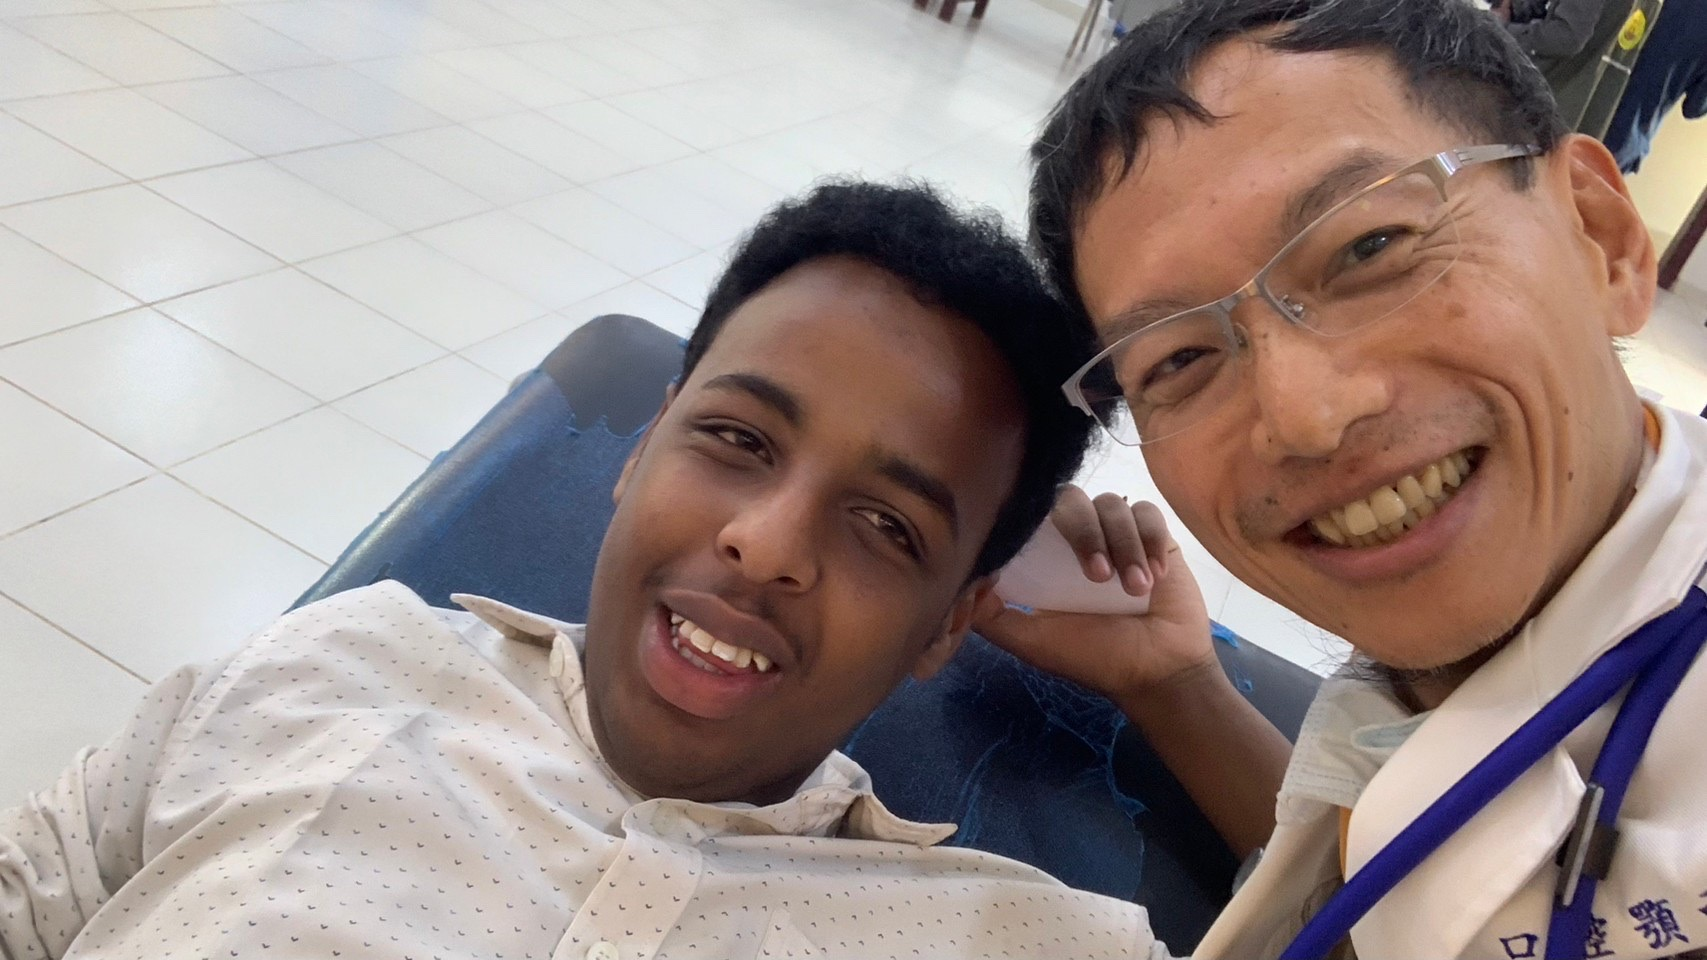
\includegraphics[width=0.25\textwidth]{IMG-5112.JPG}
    \end{center}
\end{frame}

\begin{frame}{Public health: World Blood Donor Day}
    \begin{center}
        \includesvg[width=0.2\textwidth]{Blood_logo.svg}
        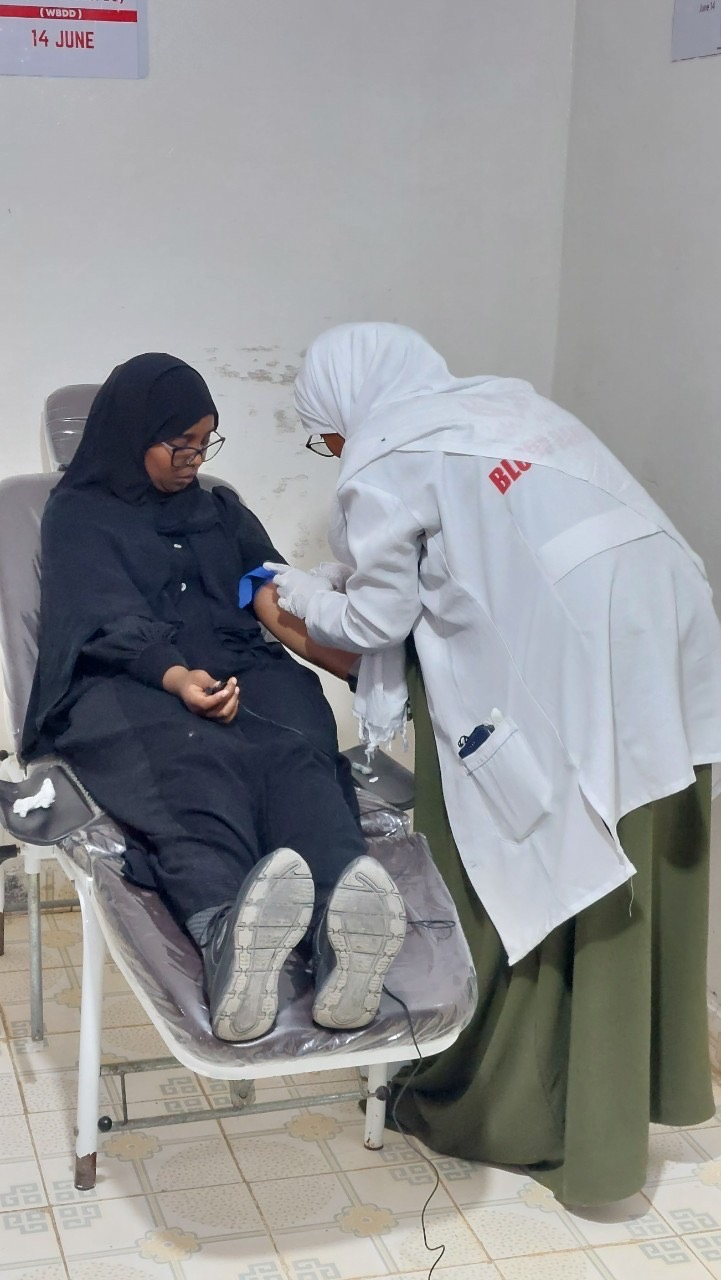
\includegraphics[width=0.30\textwidth]{IMG-4371.JPG}
        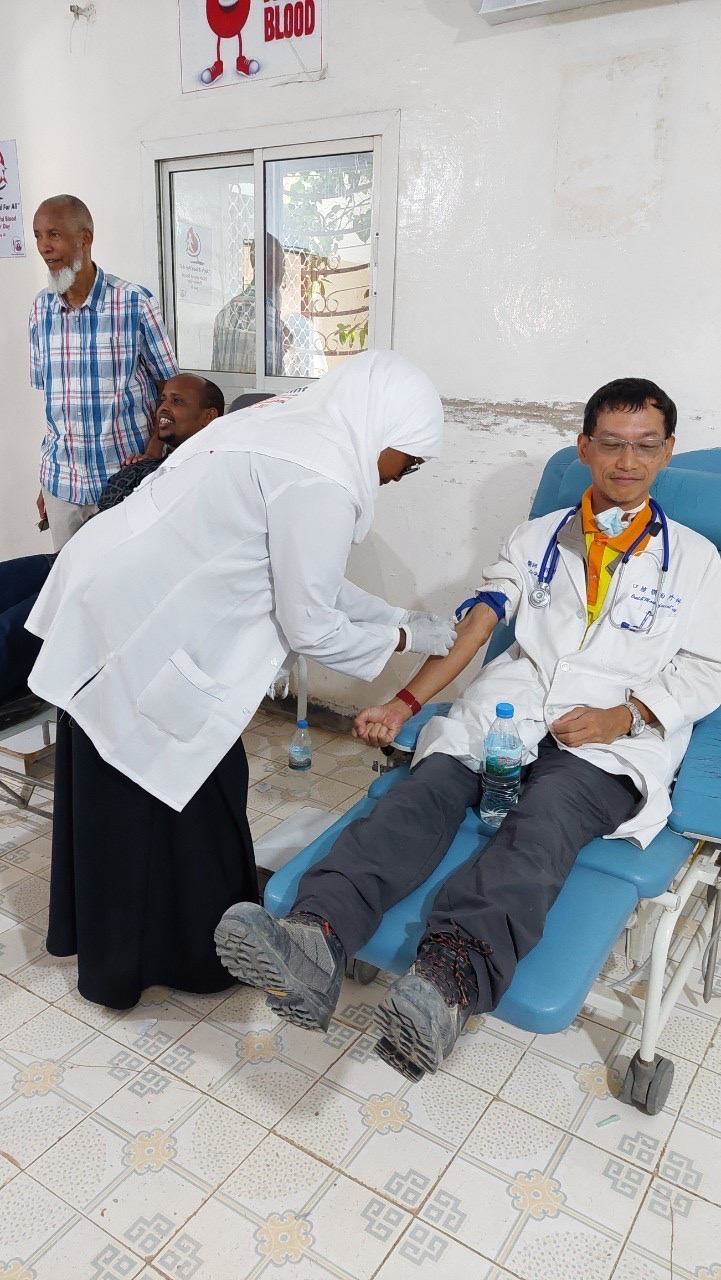
\includegraphics[width=0.30\textwidth]{IMG-4370.JPG}
    \end{center}
\end{frame}

\begin{frame}{Public health: World Blood Donor Day}
    \begin{center}
        \includesvg[width=0.2\textwidth]{Blood_logo.svg}
        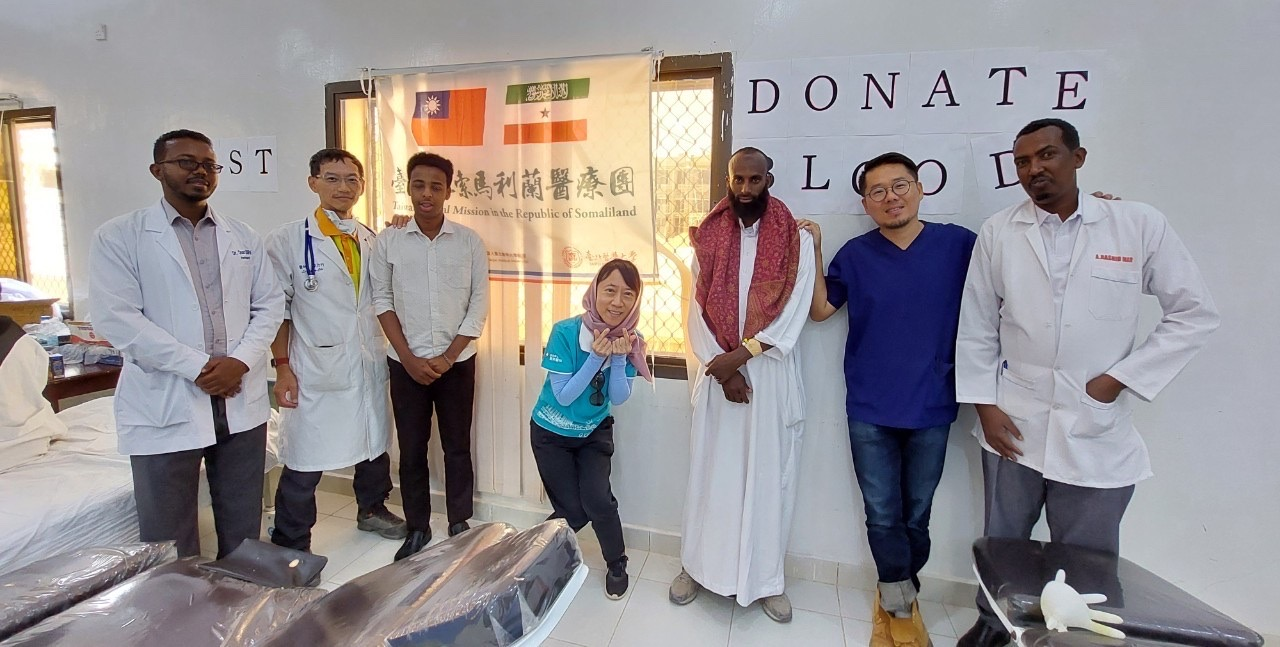
\includegraphics[width=0.75\textwidth]{IMG-4441.JPG}
%        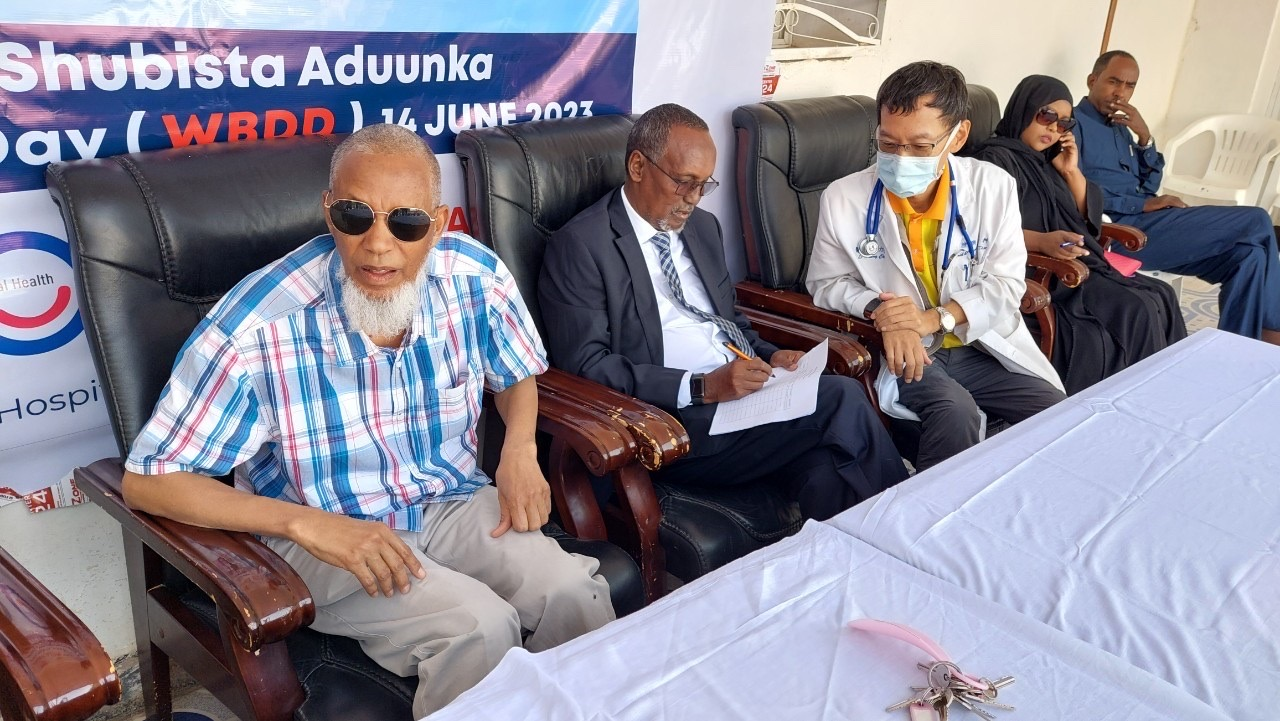
\includegraphics[width=0.45\textwidth]{IMG-4378.JPG}
    \end{center}
\end{frame}


\begin{frame}{Public health: Pap smear program since 2023/07/11}
    \begin{center}
        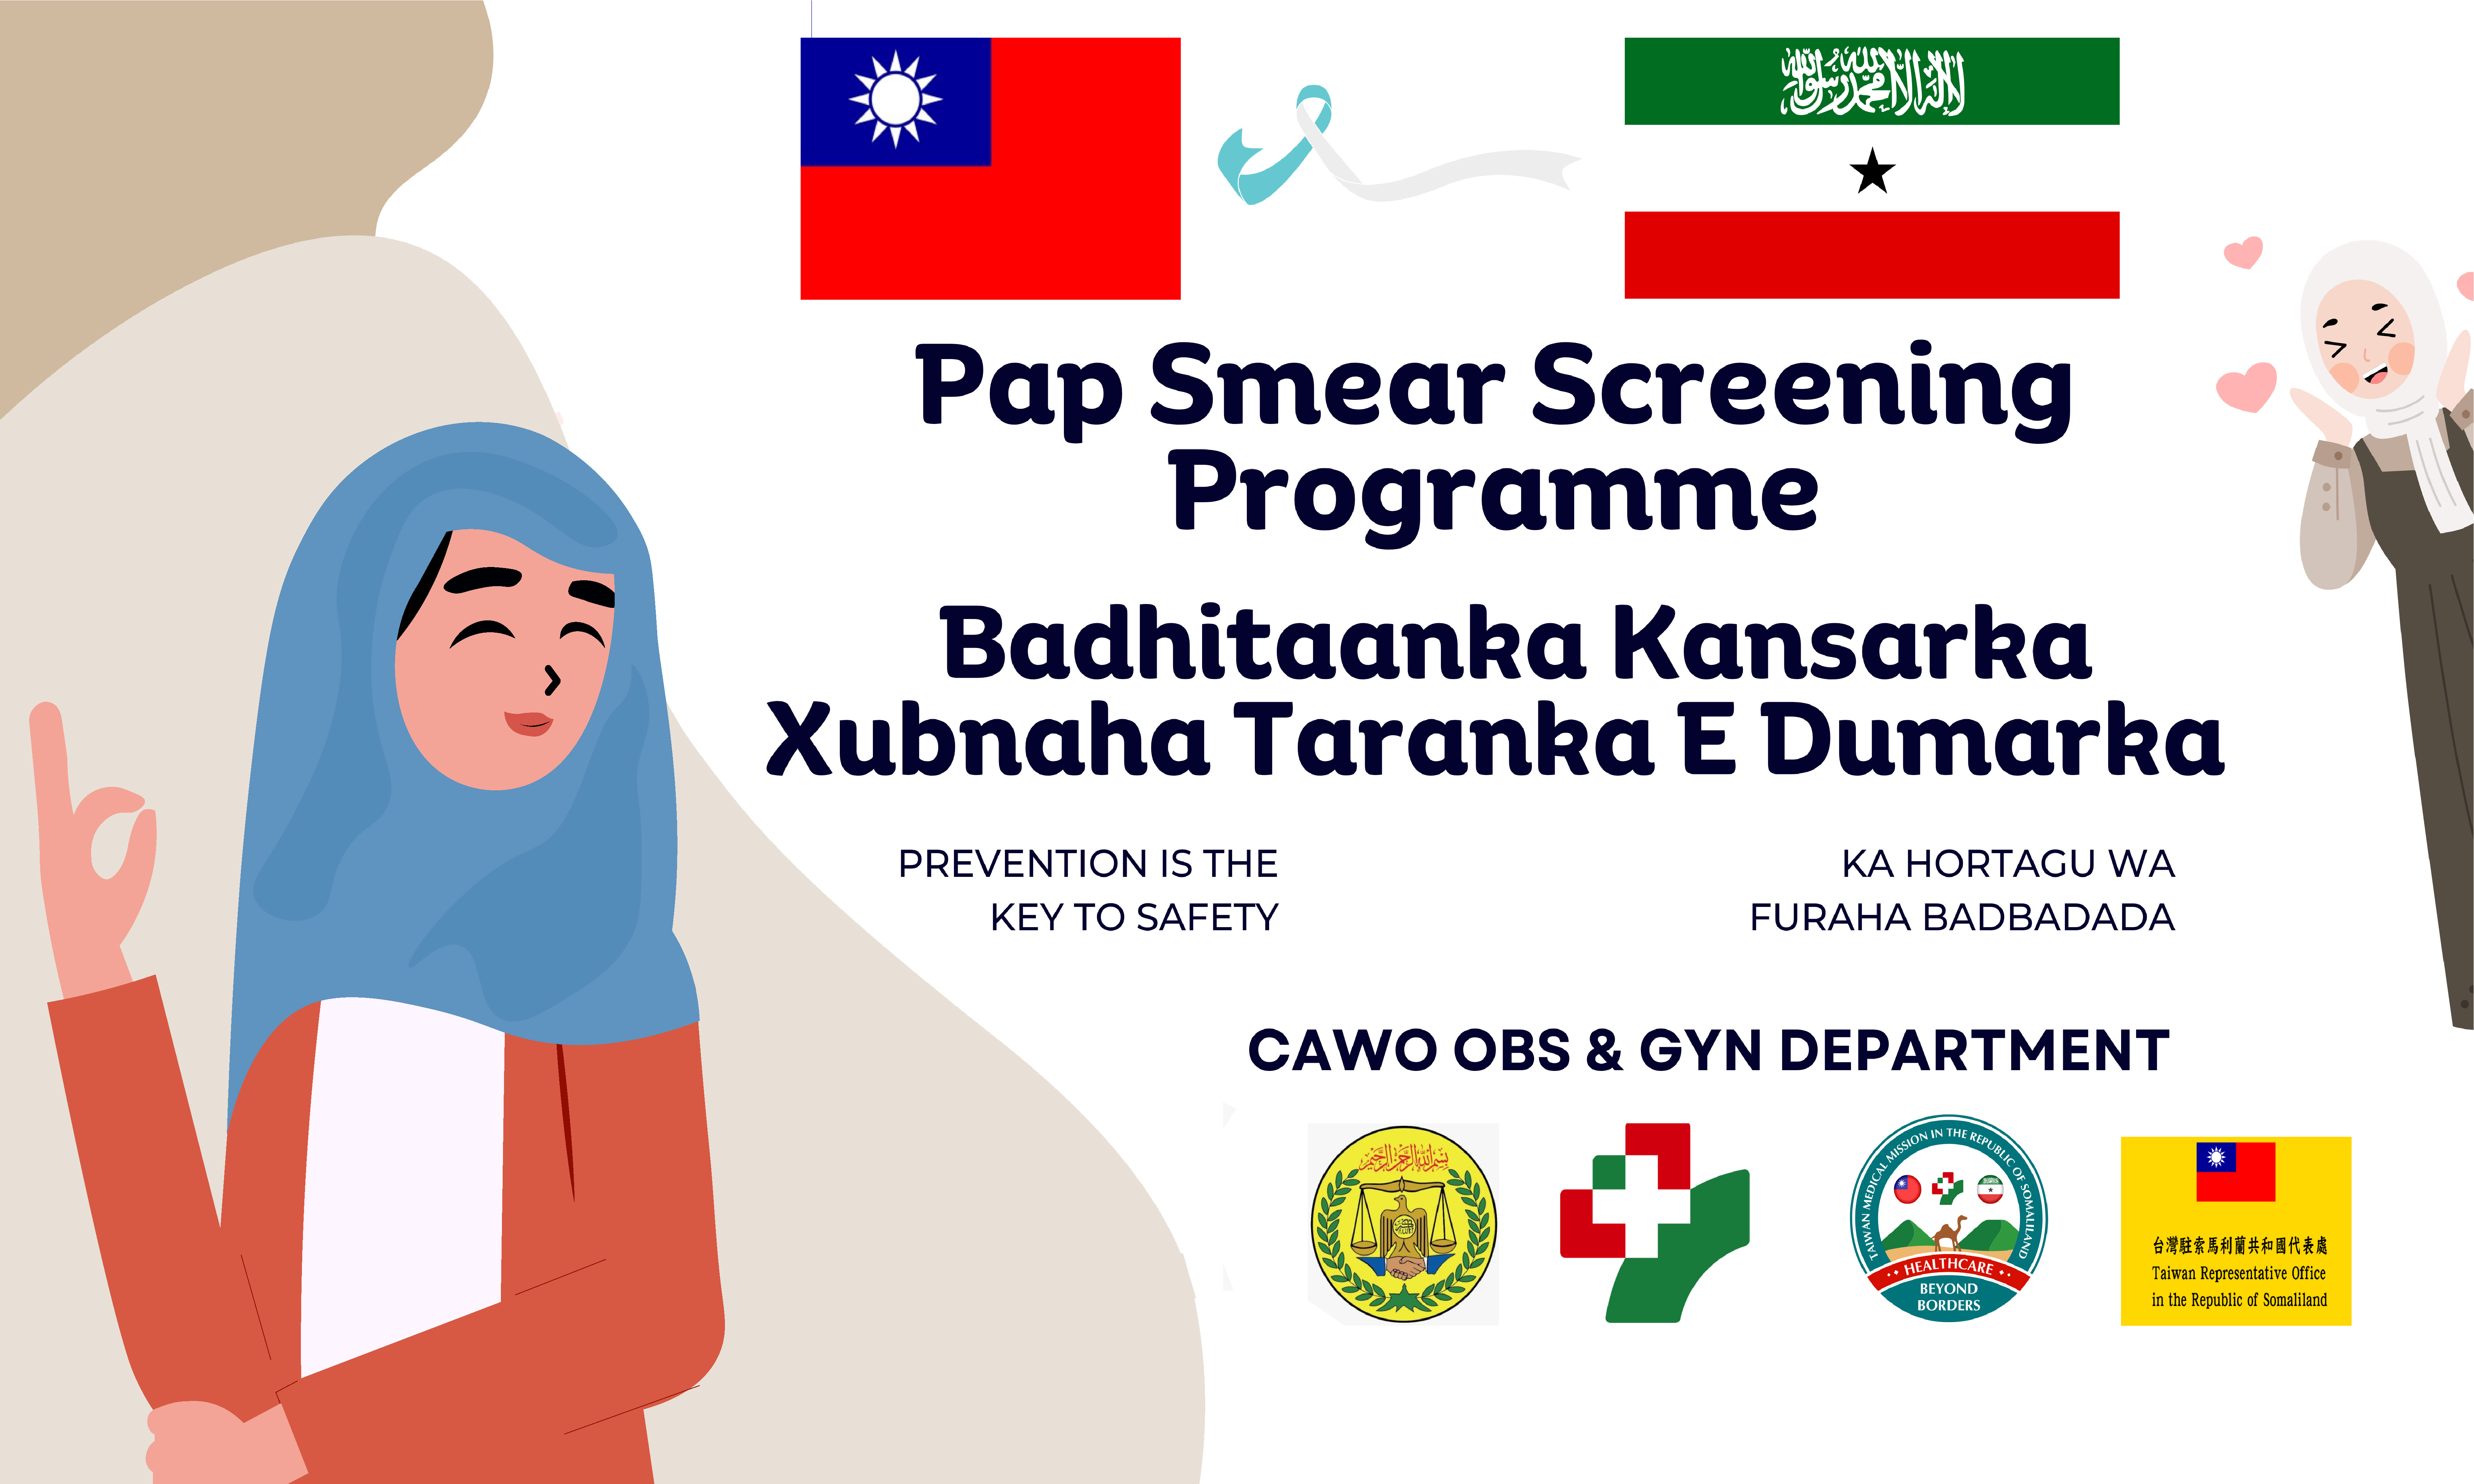
\includegraphics[width=4.5cm, height=6.5cm]{IMG-5434.JPG} 
        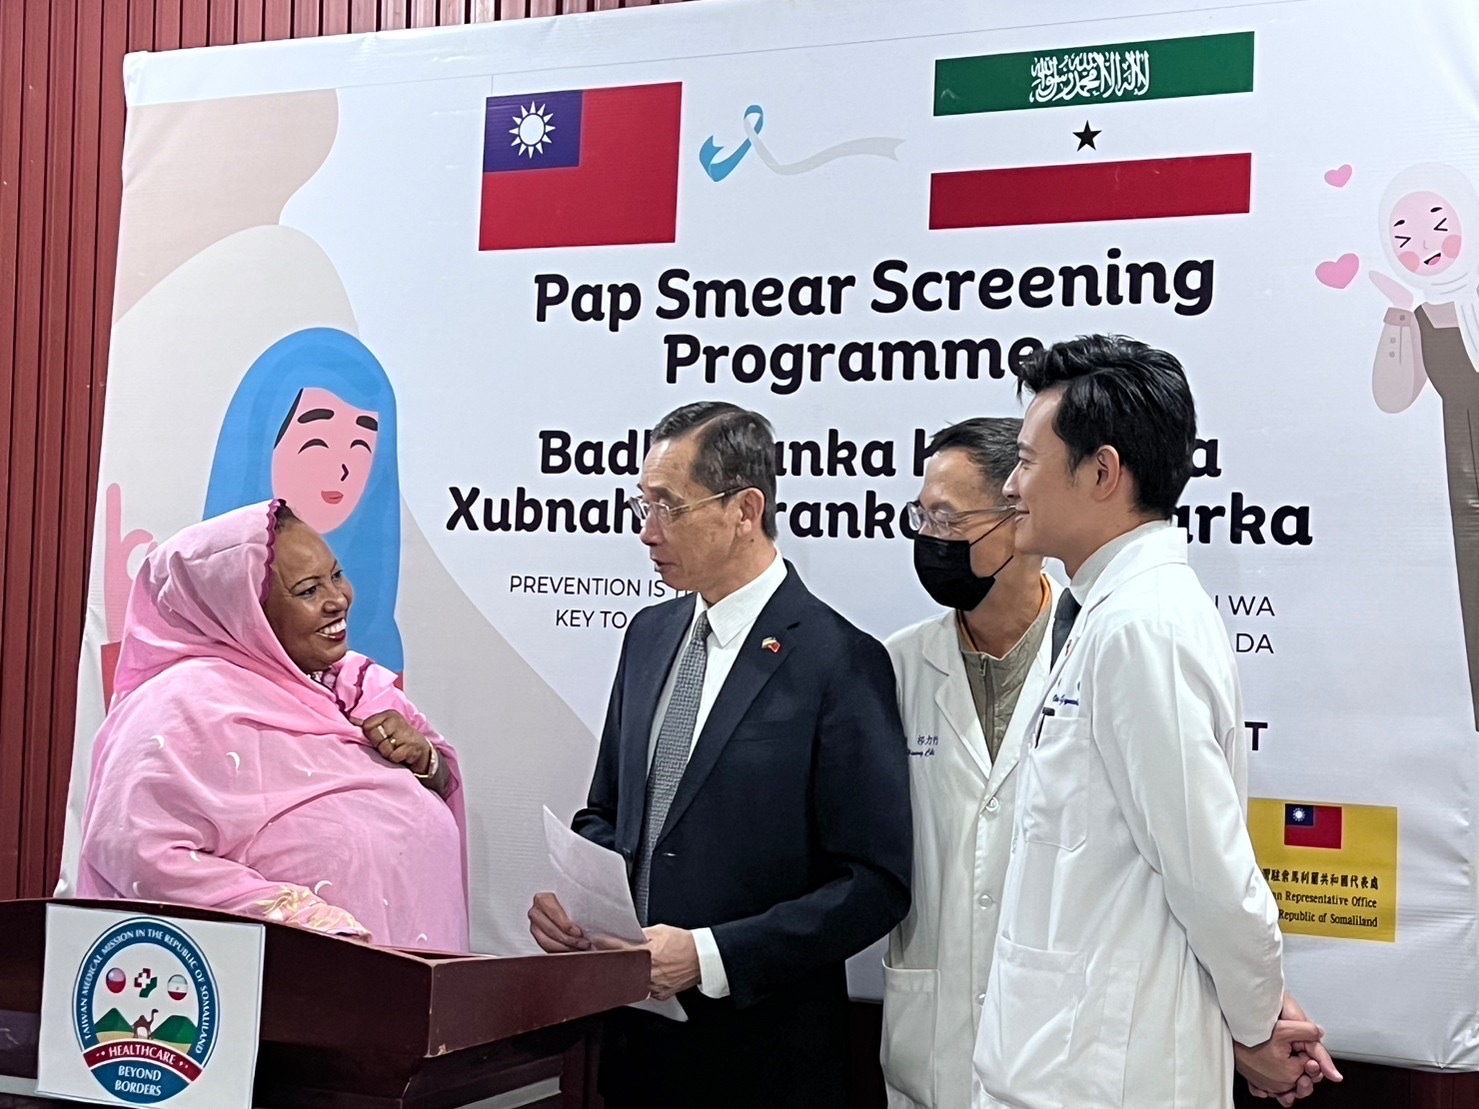
\includegraphics[width=0.6\textwidth]{IMG-5436.JPG}
%        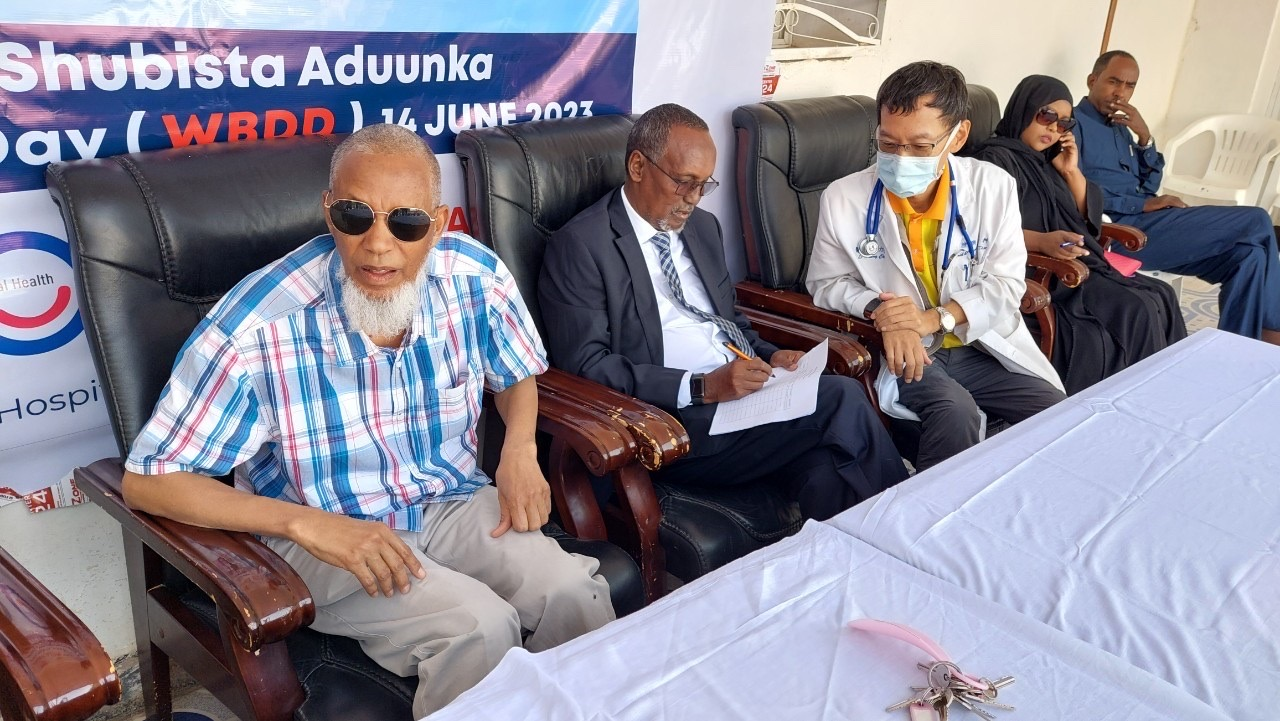
\includegraphics[width=0.45\textwidth]{IMG-4378.JPG}
    \end{center}
\end{frame}


\begin{frame}{Public health: Pap smear program (Dr. Dave Lin)}
    \begin{center}
%        \includesvg[width=0.2\textwidth]{Blood_logo.svg}
        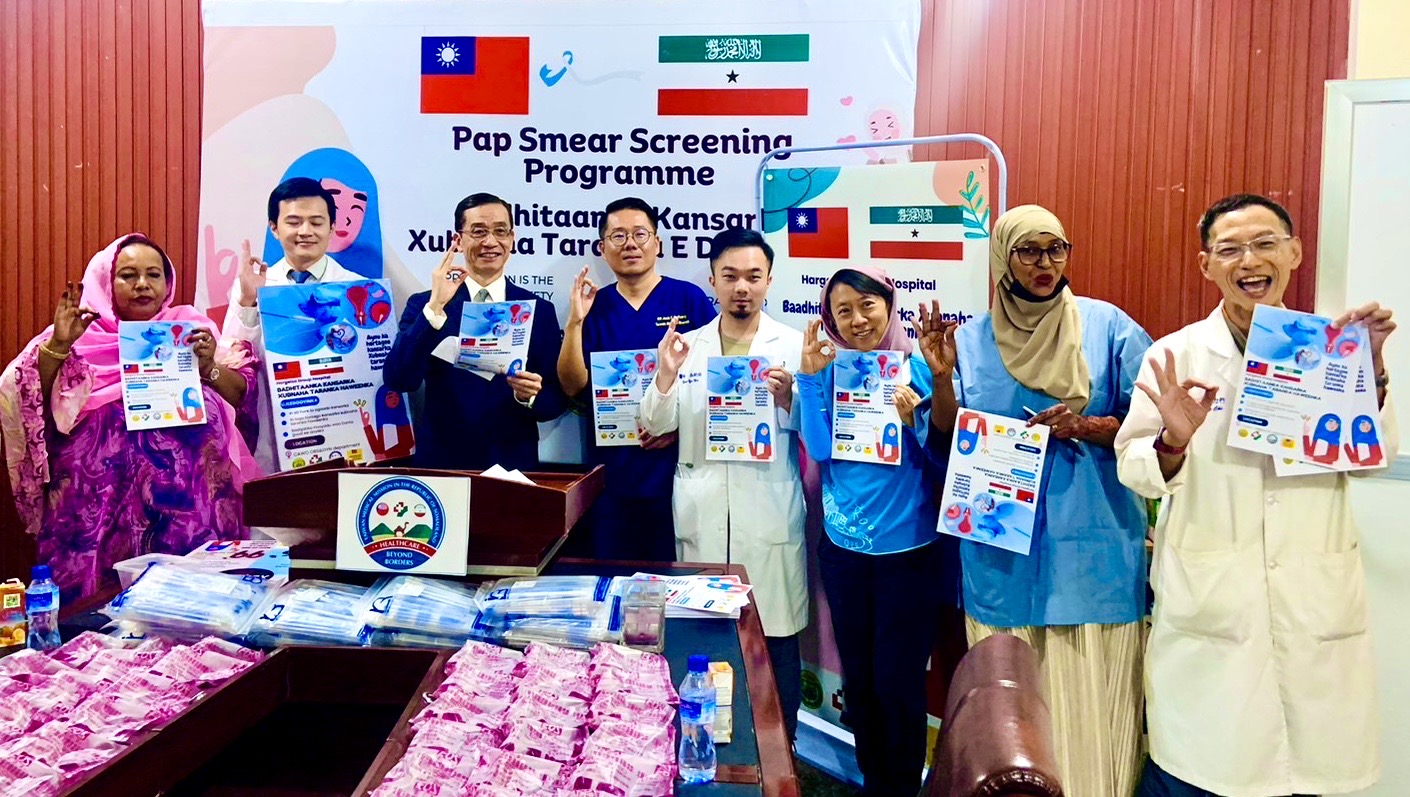
\includegraphics[width=0.95\textwidth]{IMG-5437.JPG}
%        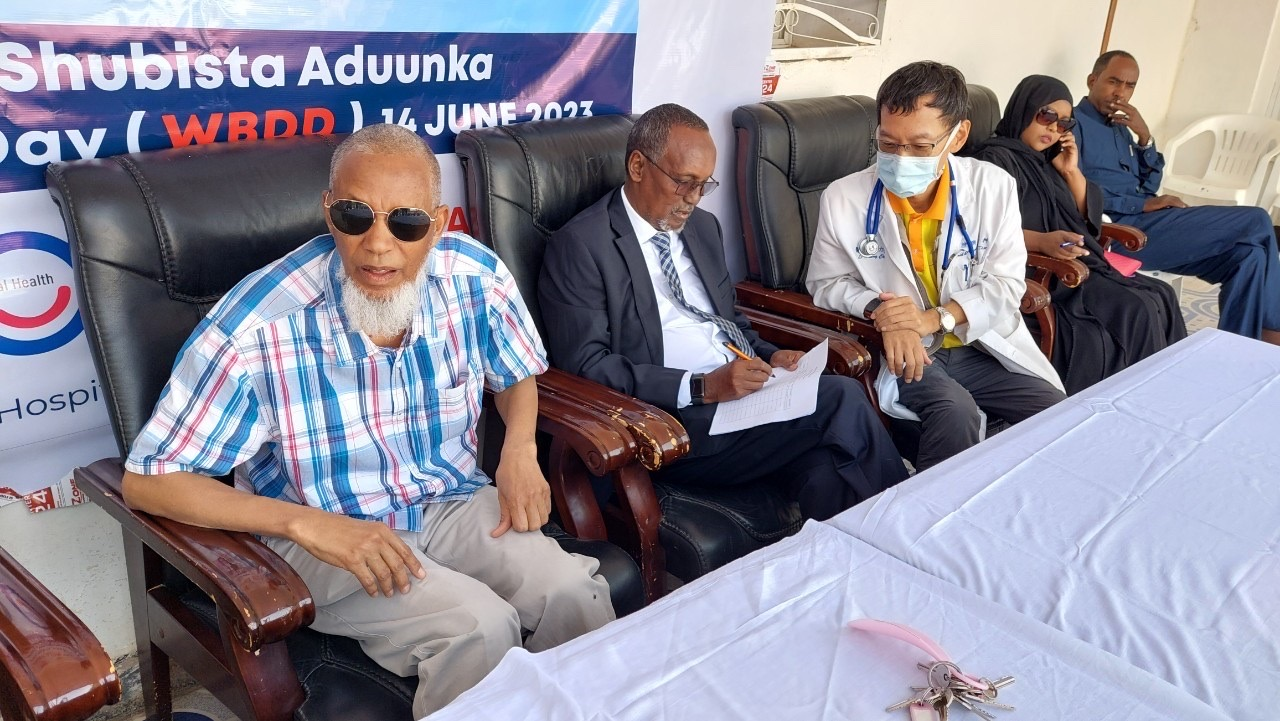
\includegraphics[width=0.45\textwidth]{IMG-4378.JPG}
    \end{center}
\end{frame}
%%%

\begin{frame}
\frametitle{TMM's Projects - fourth pillar}
% Add content here
\begin{outline}    
    \1 telemedicine
        \2 by collaborating with specialists at TMU affiliated Hospitals
        \2 \textcolor{red}{telepathology} project with a pathologist through digital whole-slide images (WSIs)
        \2 \textcolor{red}{"RadiPush"} project to fasciliate last-mile transfer of radiologist reports to doctors; for example: Taiwan Osteoporosis Master (TOM) for T-score
    
\end{outline}
\end{frame}


\begin{frame}{Telepathology and Radiology}
    \begin{center}
        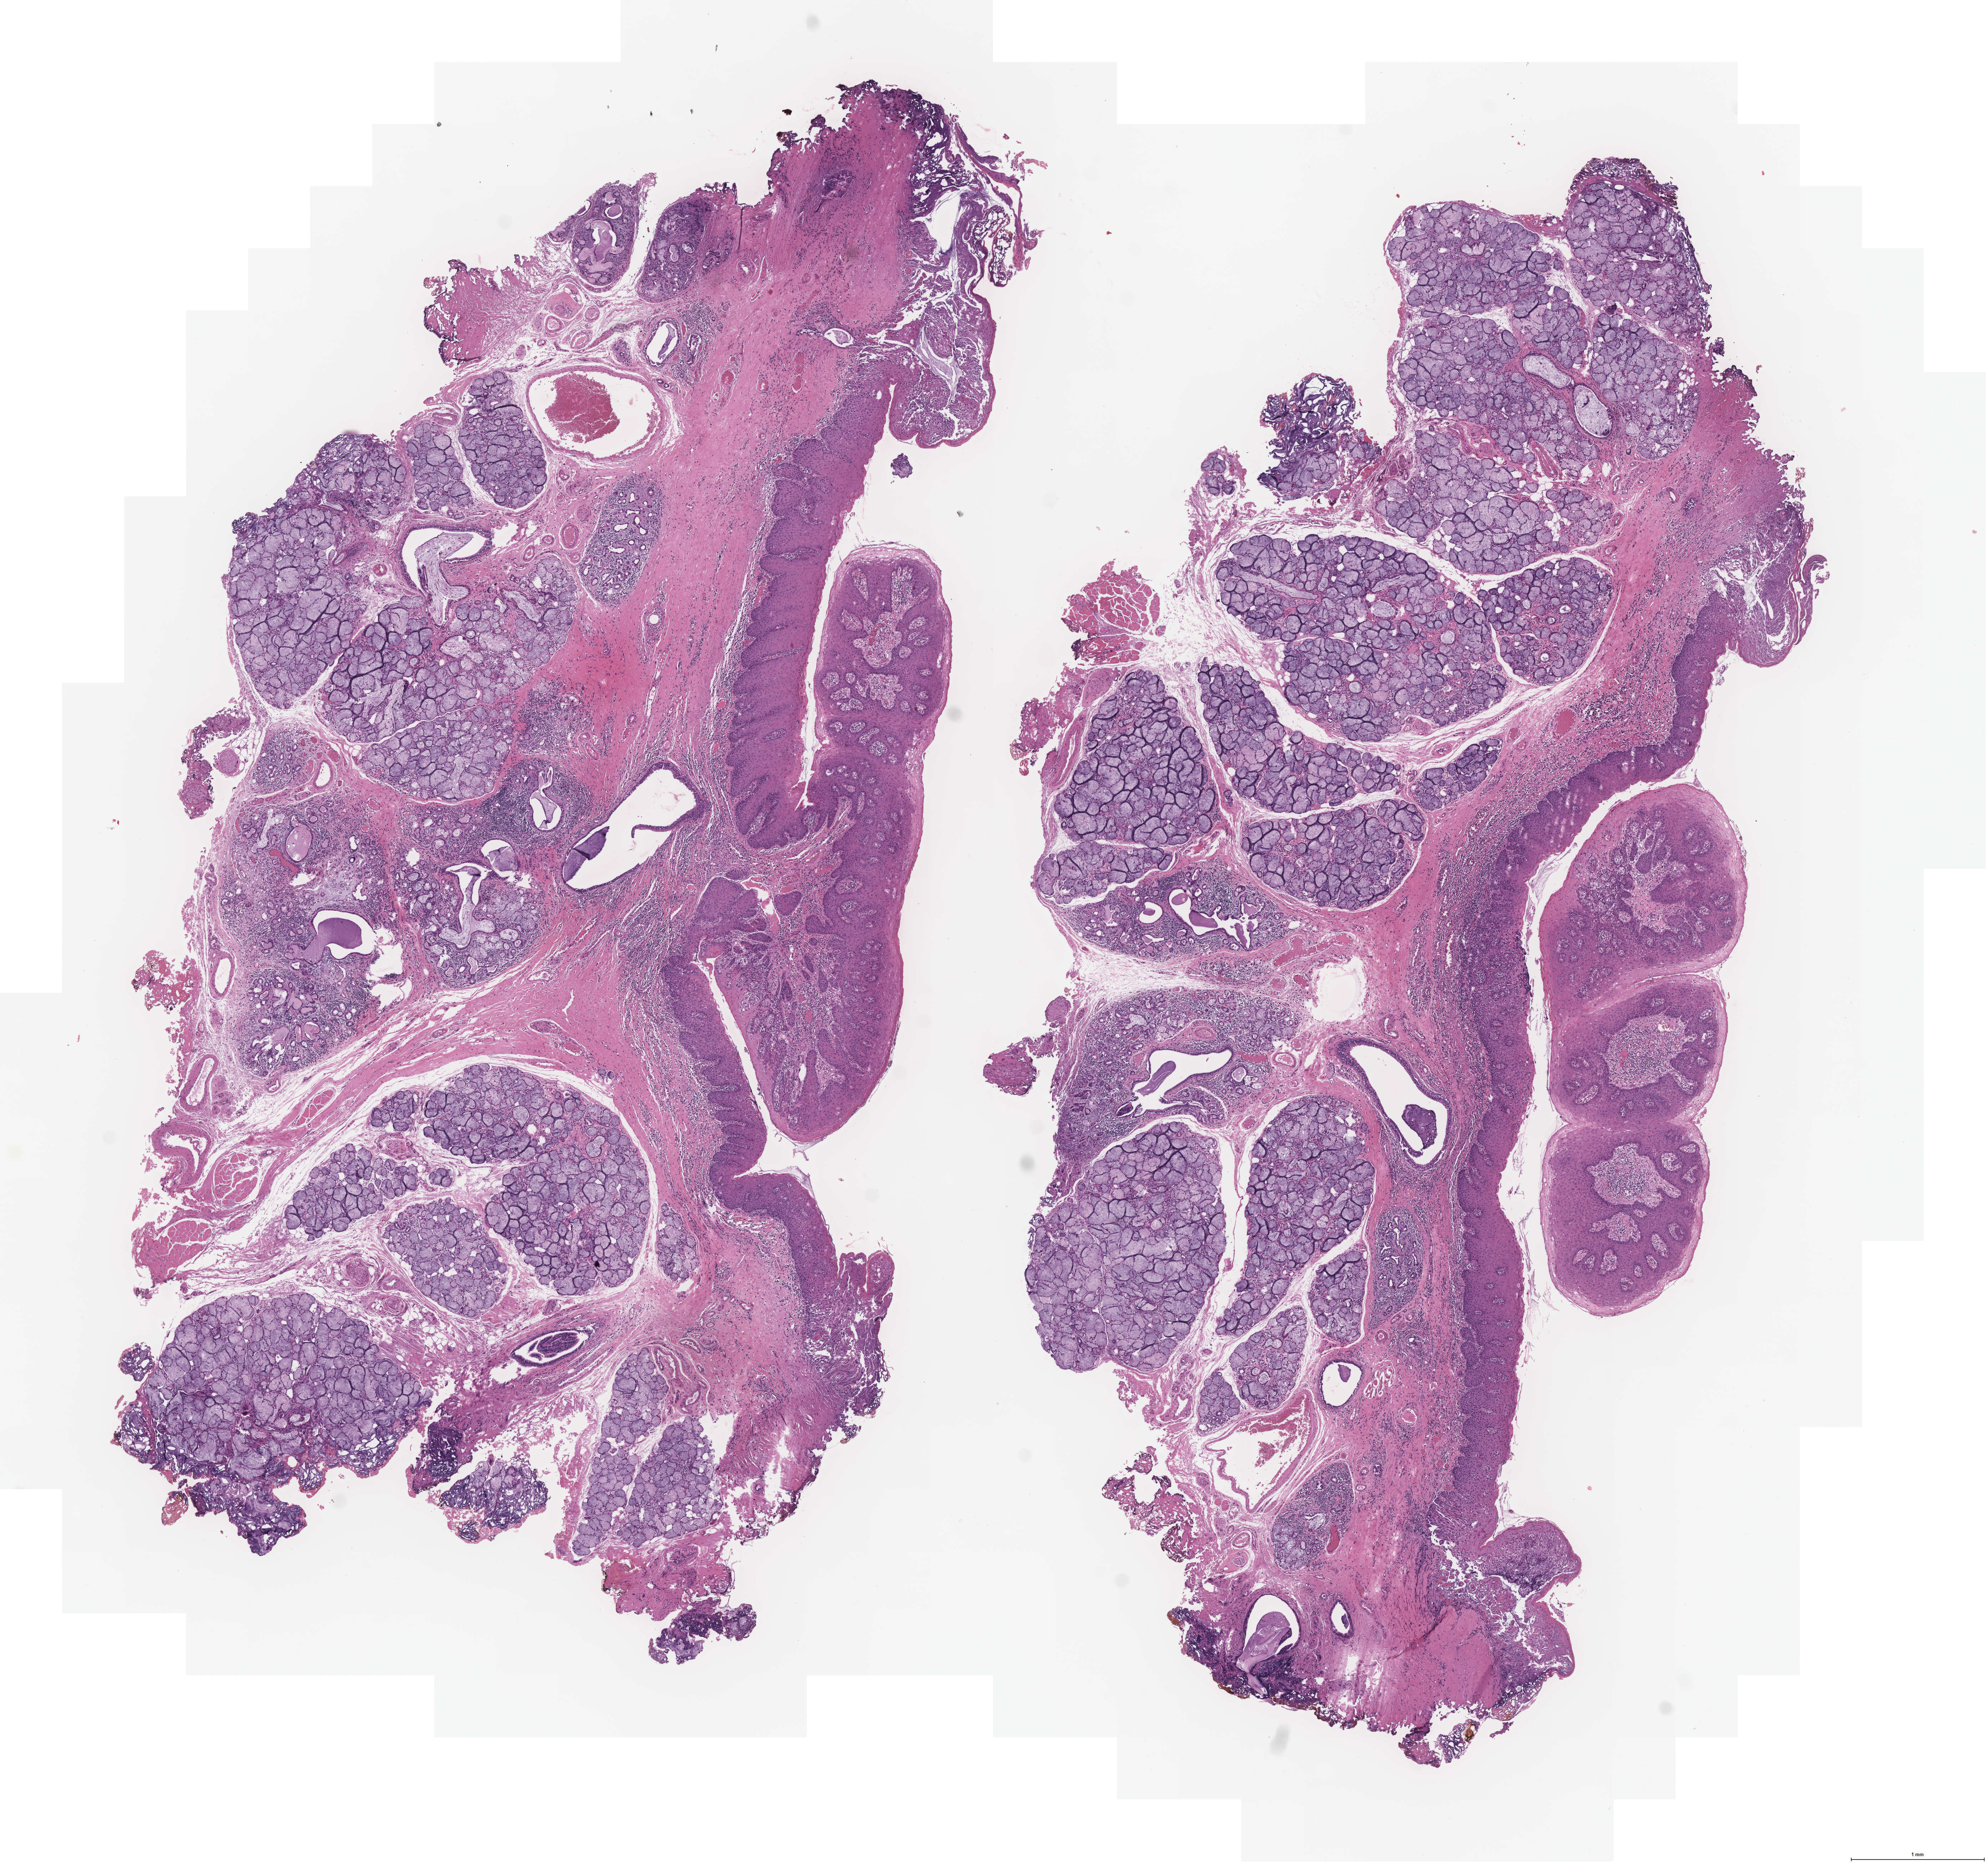
\includegraphics[width=0.35\textwidth]{TH1919729C1_HE.jpeg}
        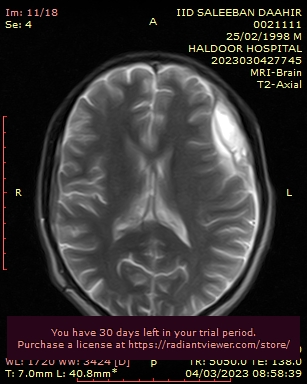
\includegraphics[width=0.30\textwidth]{IMG-0007-00001.jpg}
    \end{center}
\end{frame}


\begin{frame}{Teleconsultation: non-human vertebrae (cheetah)}
    \begin{center}
        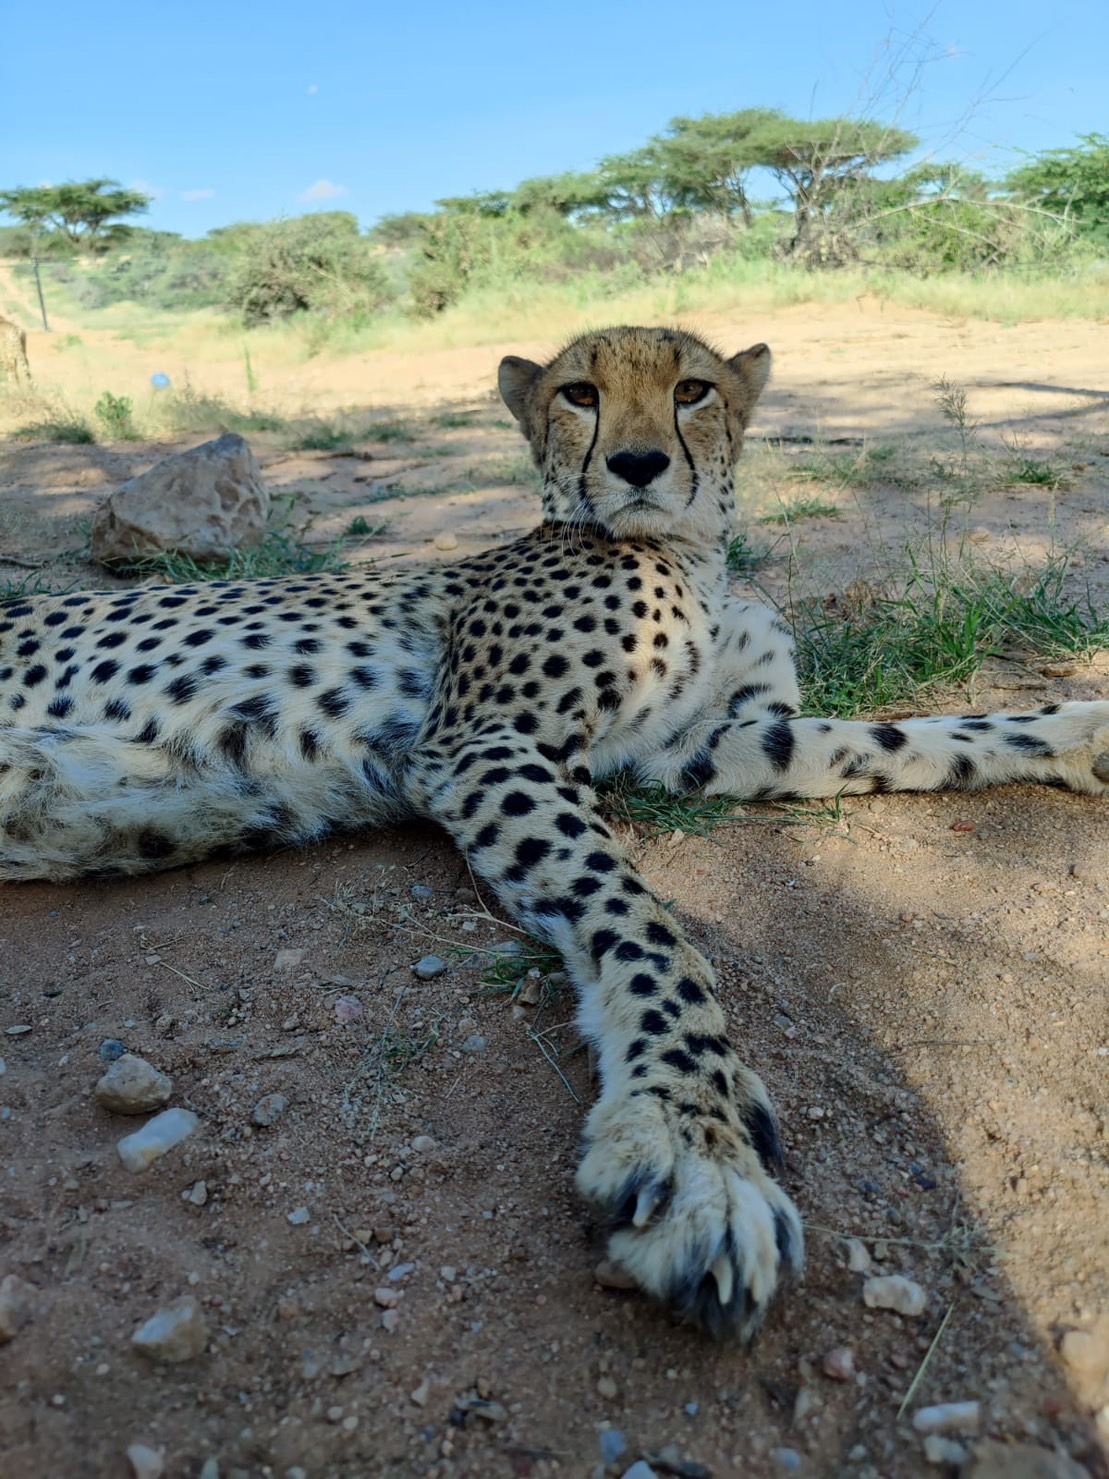
\includegraphics[width=0.35\textwidth]{457256160987709682.jpg}        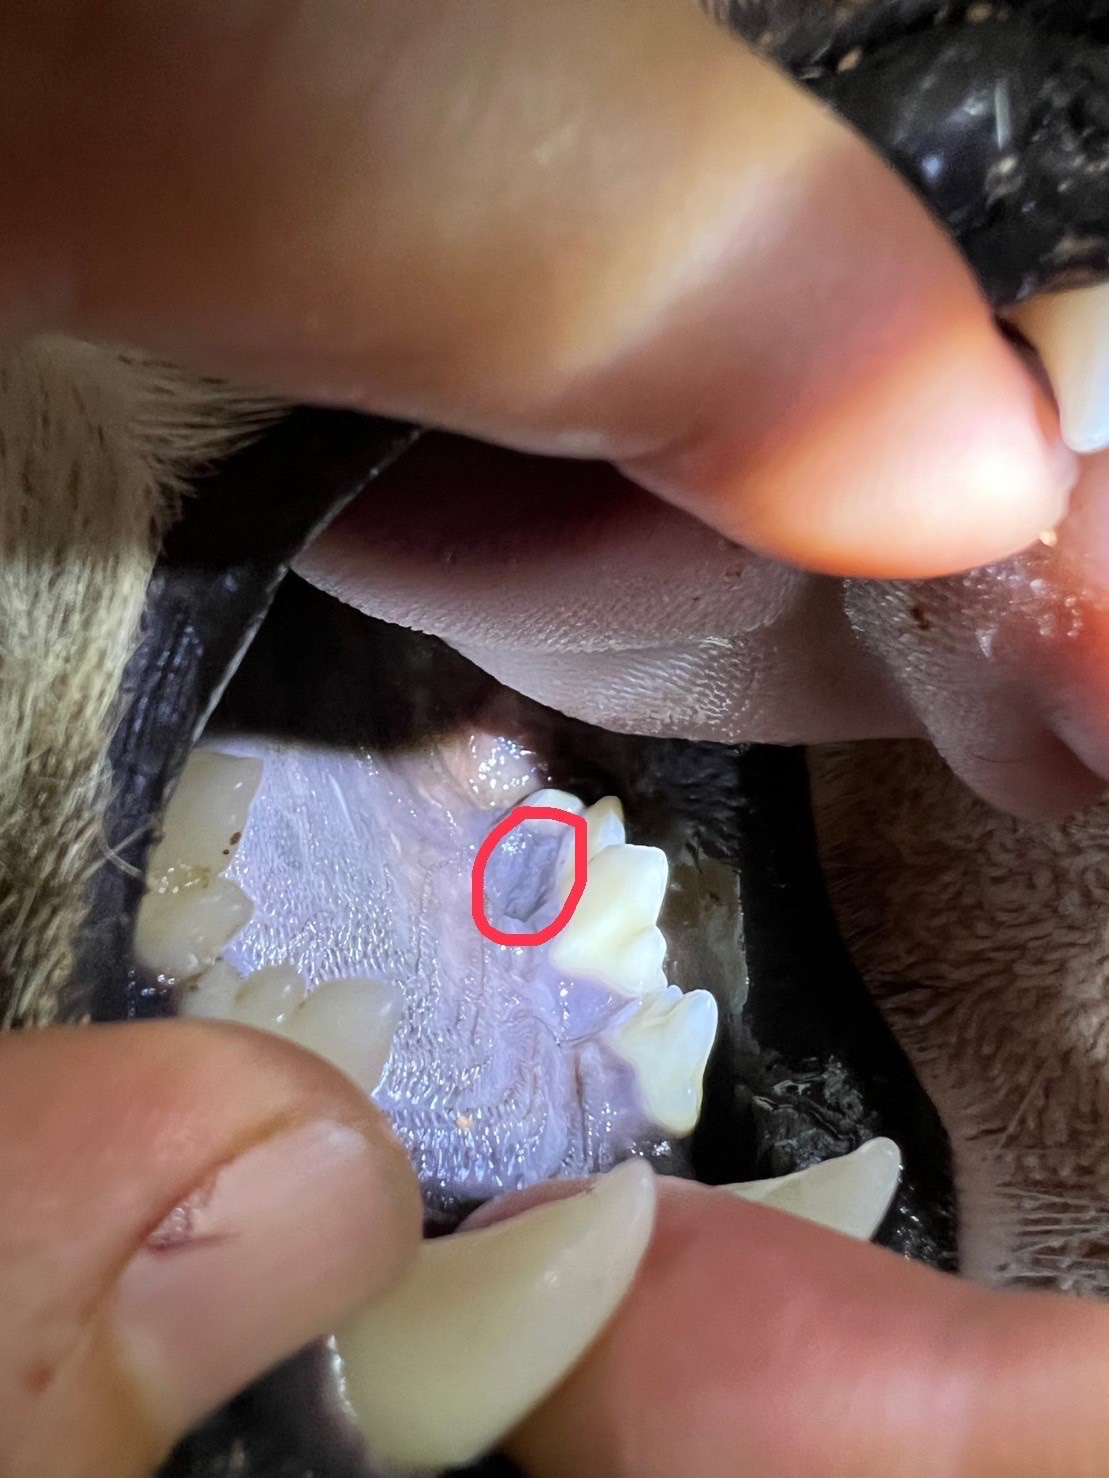
\includegraphics[width=0.35\textwidth, origin=c,angle=180]{IMG-5116.JPG}

    \end{center}
\end{frame}

%%%%%%%%%%%%%%%%5555

\begin{frame}{2023/07 Laas Geel, Somaliland}
    \begin{center}
        
\includegraphics[width=1.0\textwidth]{IMG-5232.jpg}
        %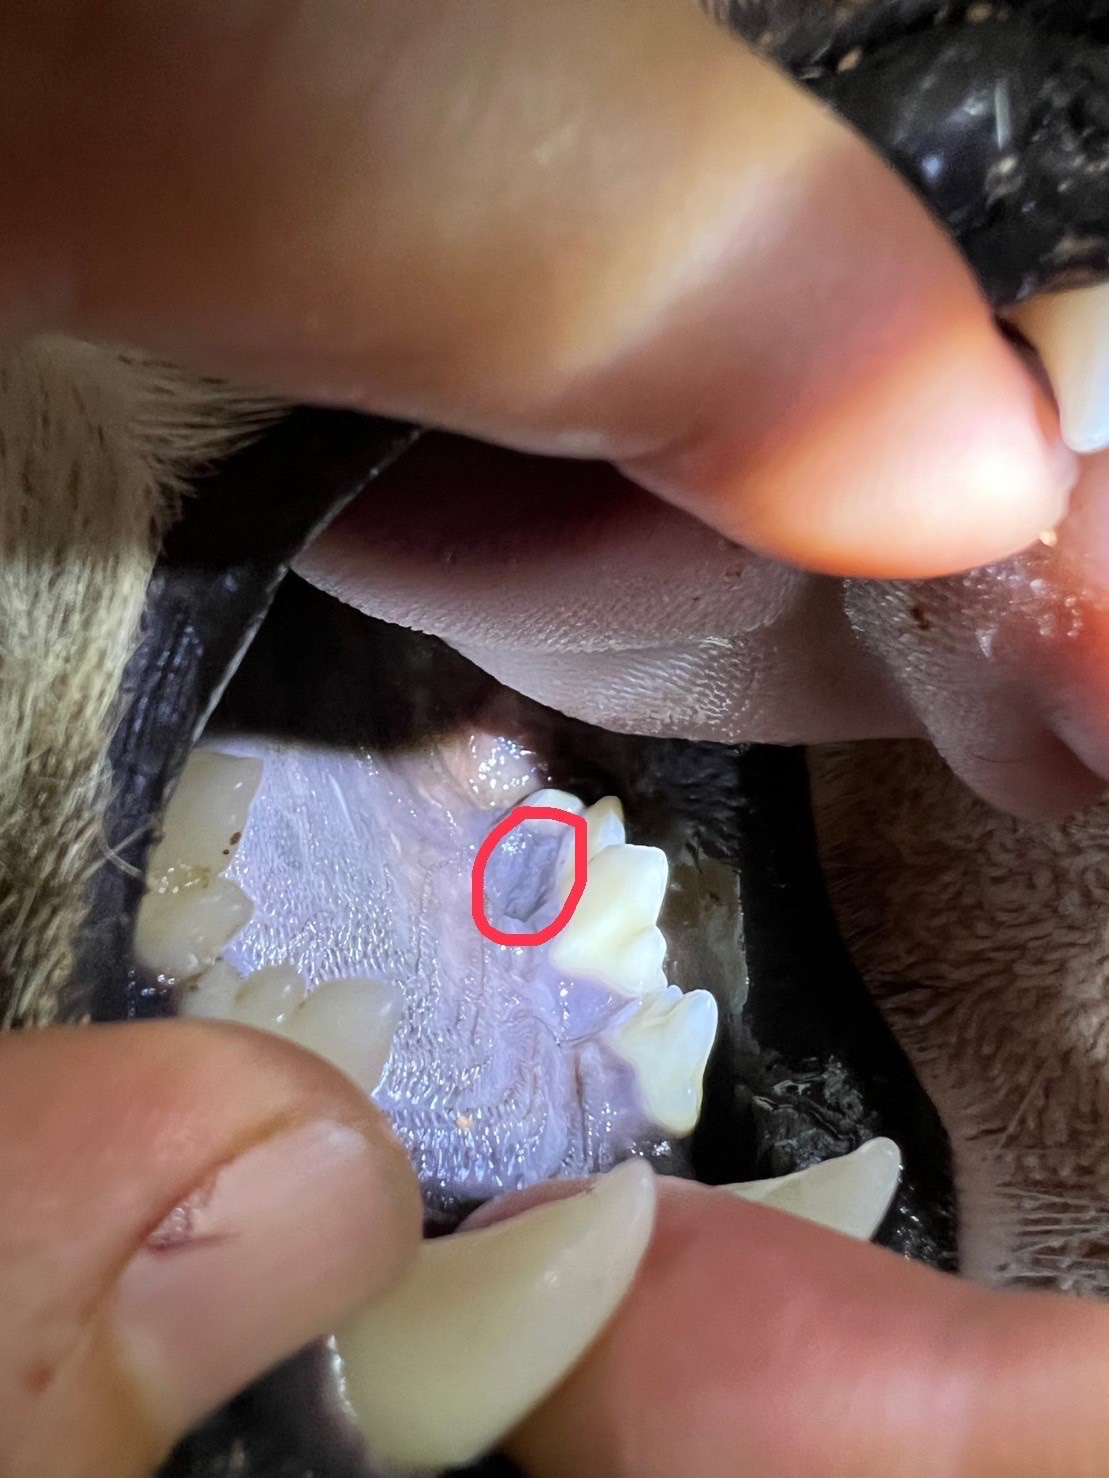
\includegraphics[width=0.85\textwidth, origin=c,angle=180]{IMG-5116.JPG}

    \end{center}

\end{frame}


\begin{frame}{2023/07 Laas Geel, Somaliland}
    \begin{center}
        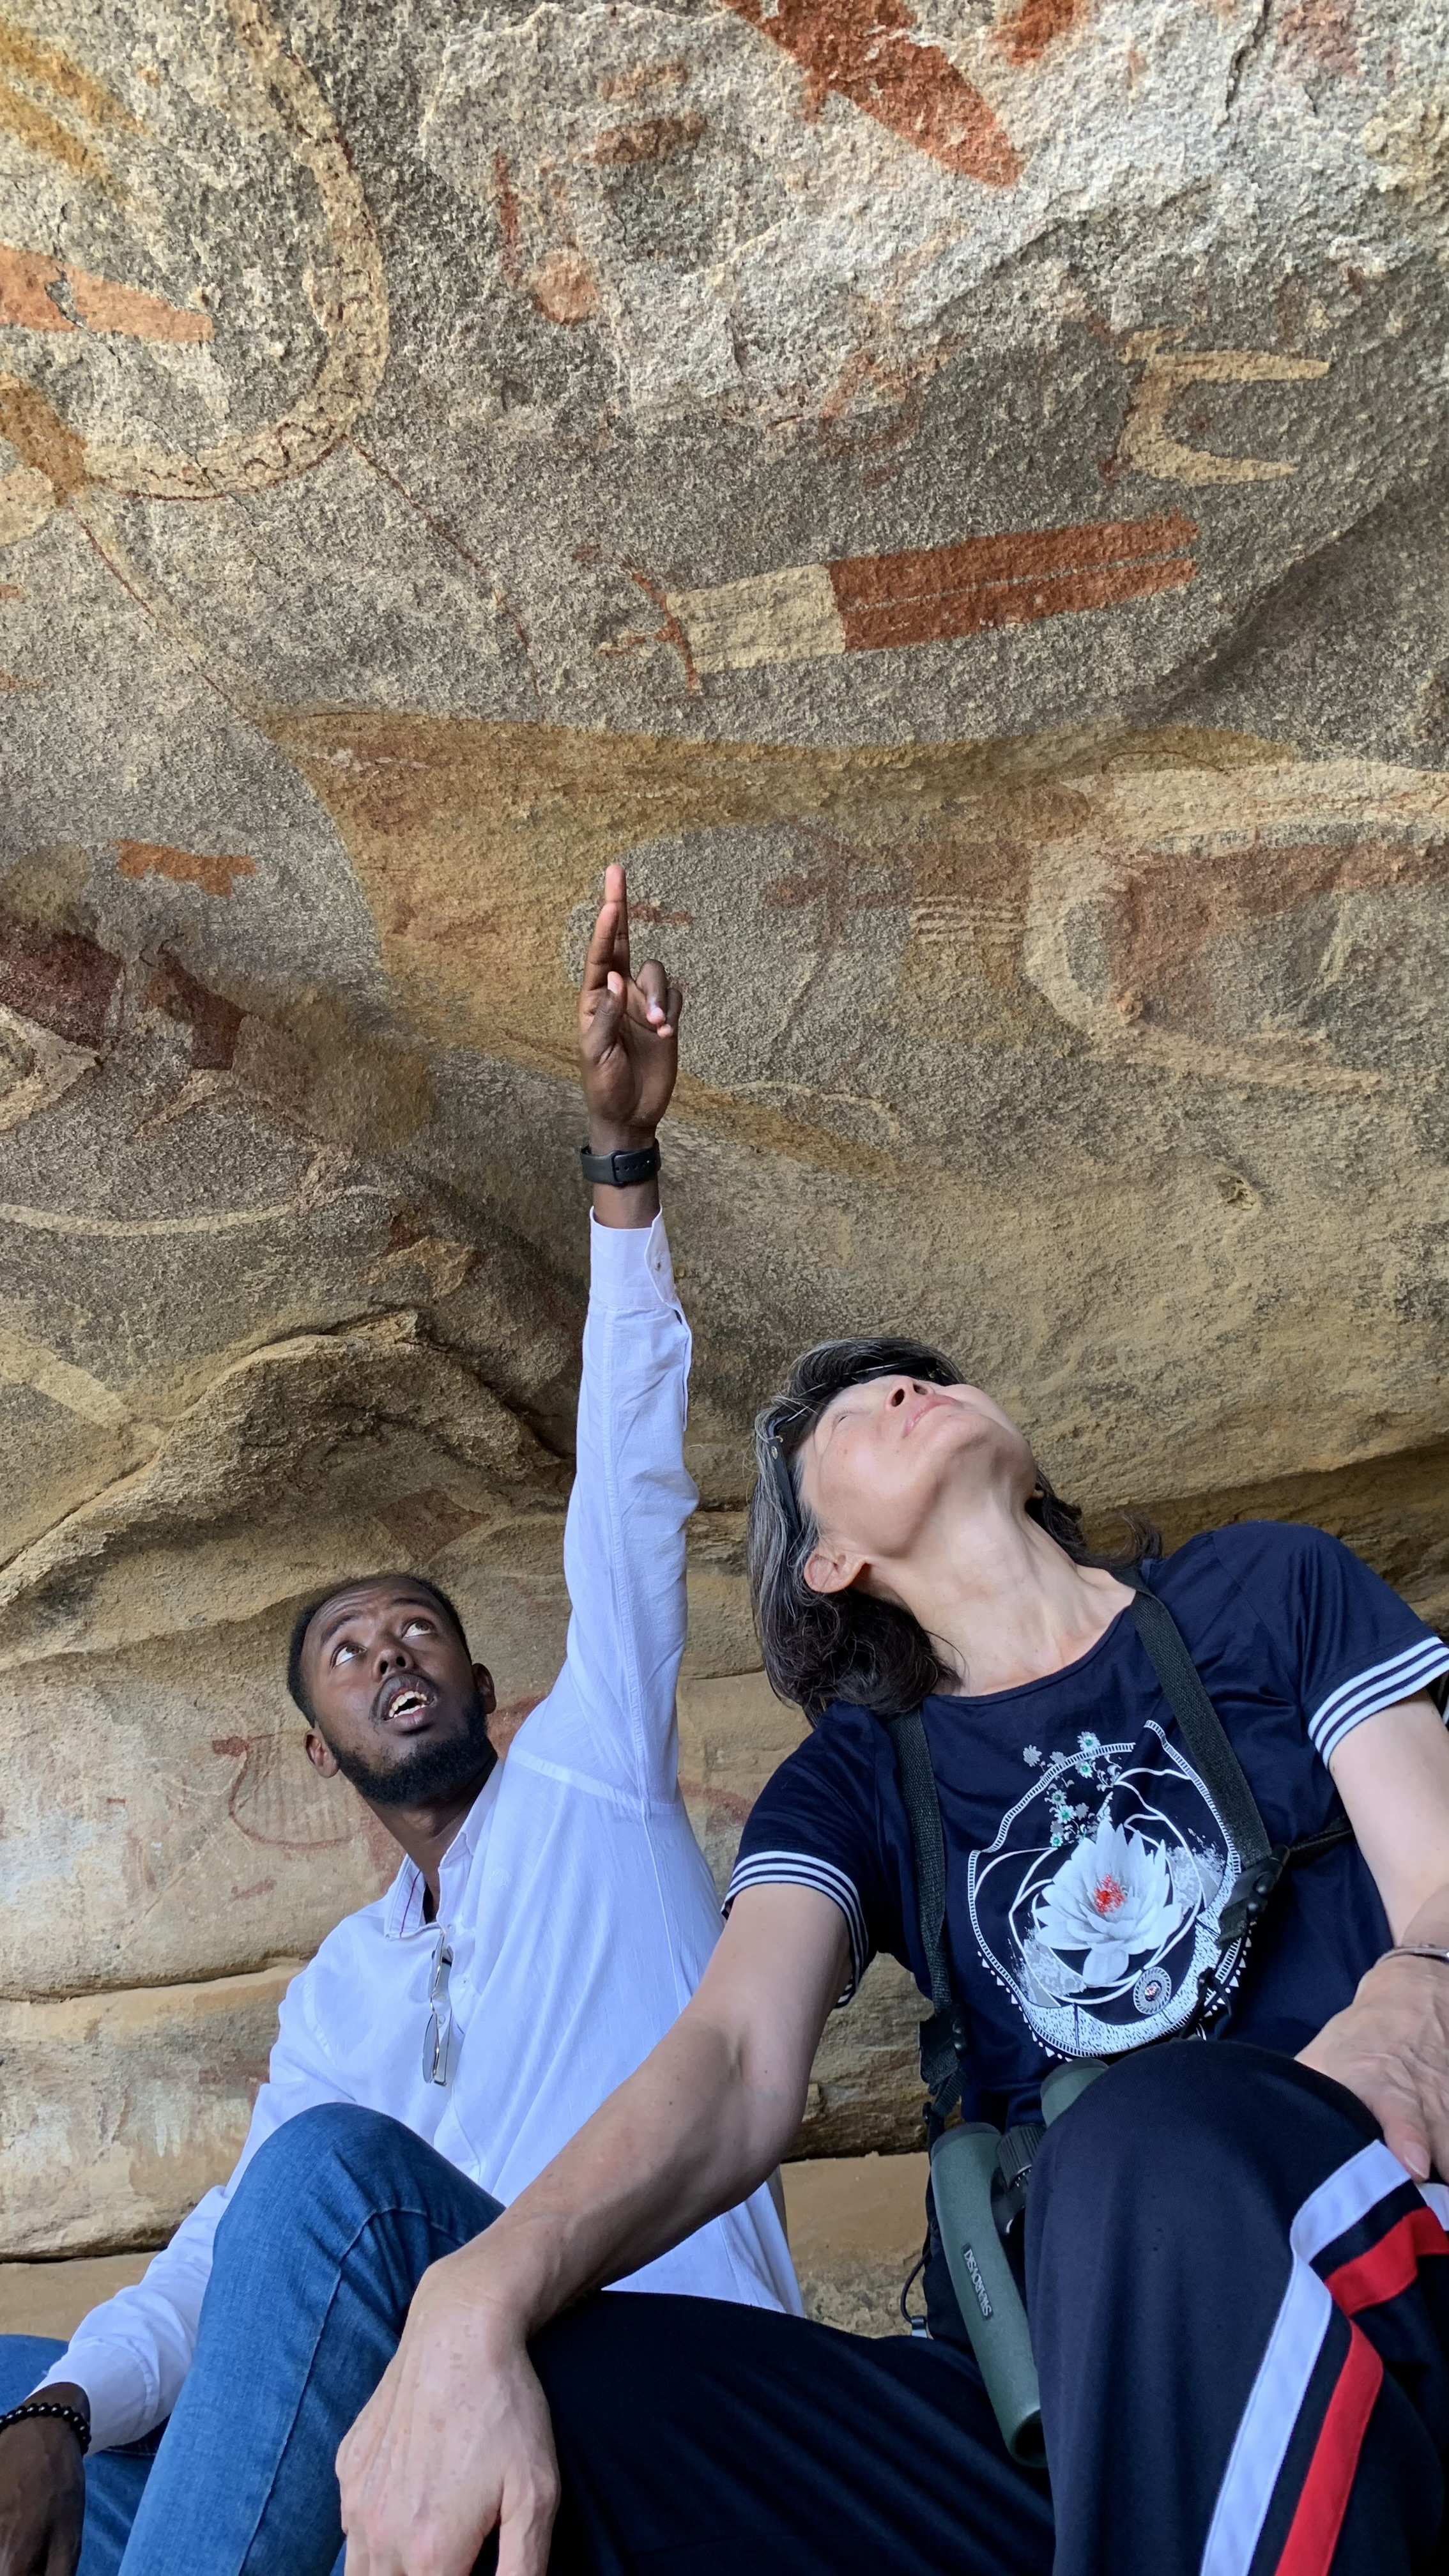
\includegraphics[width=0.25\textwidth]{IMG-5205.jpg}
        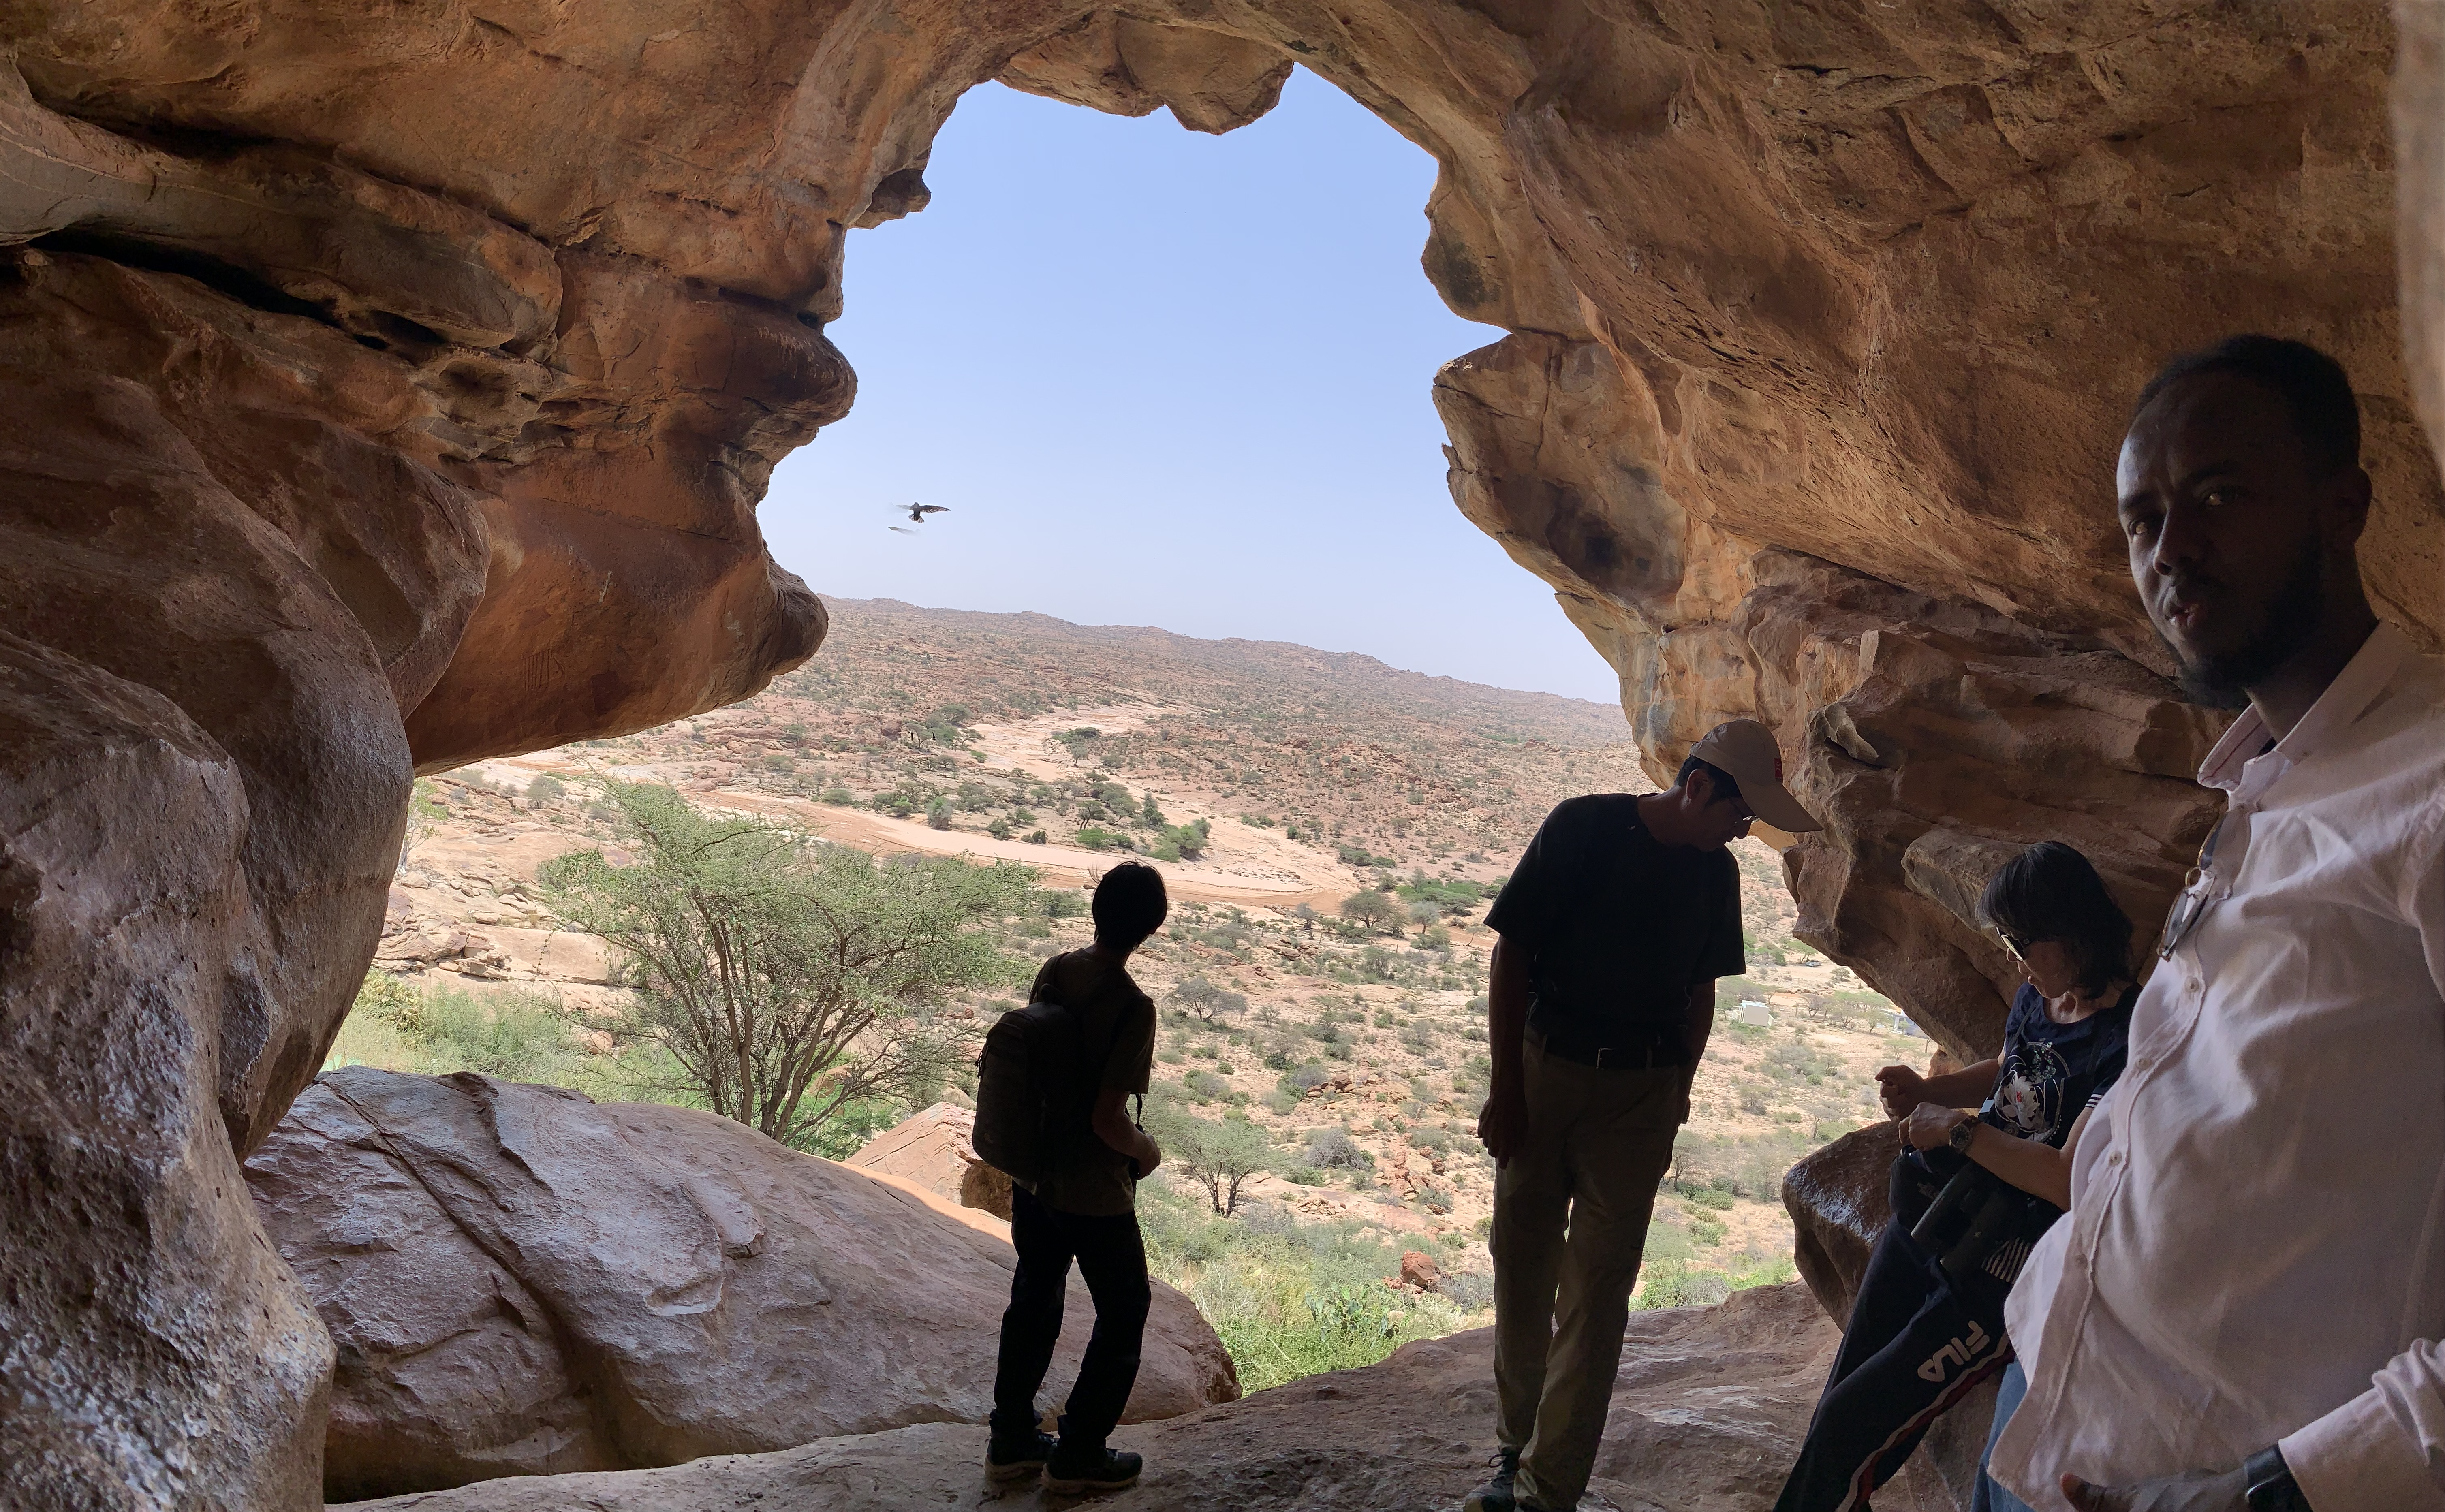
\includegraphics[width=0.55\textwidth]{IMG-5247.jpg}

    \end{center}

\end{frame}


\begin{frame}{7000-year-old tales}
    \begin{center}
        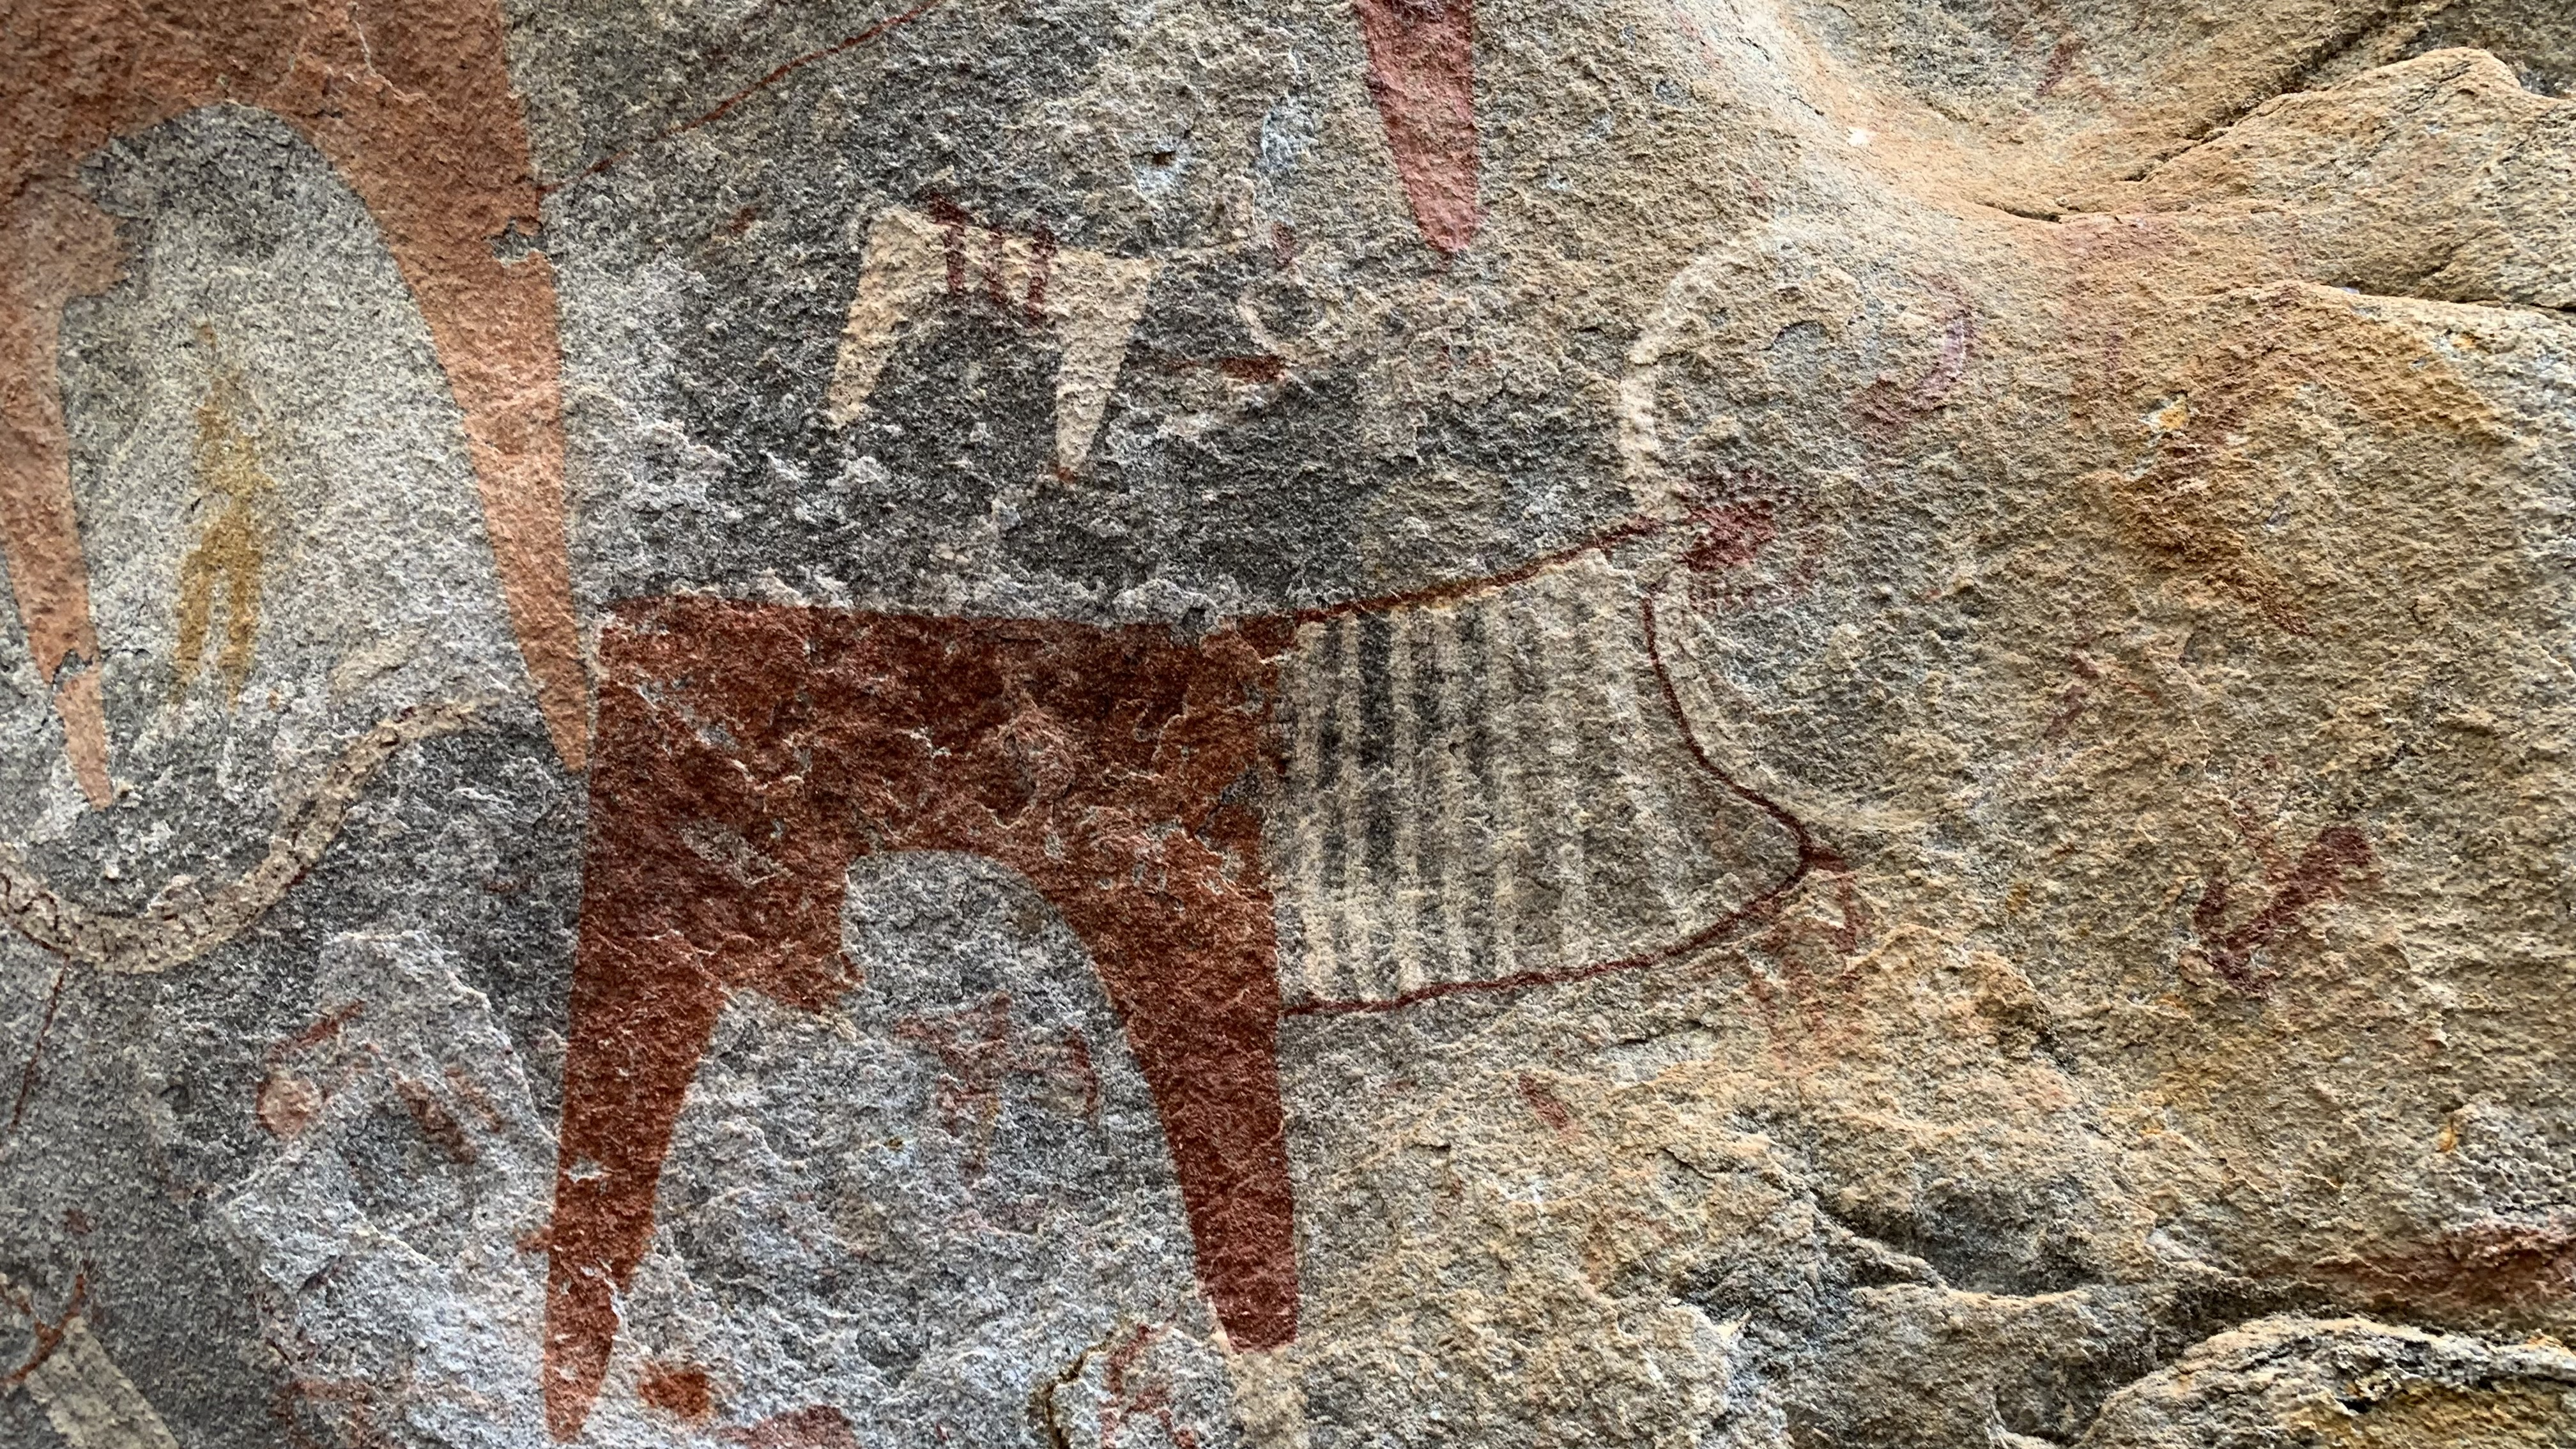
\includegraphics[width=0.45\textwidth]{IMG-5204.jpg}
        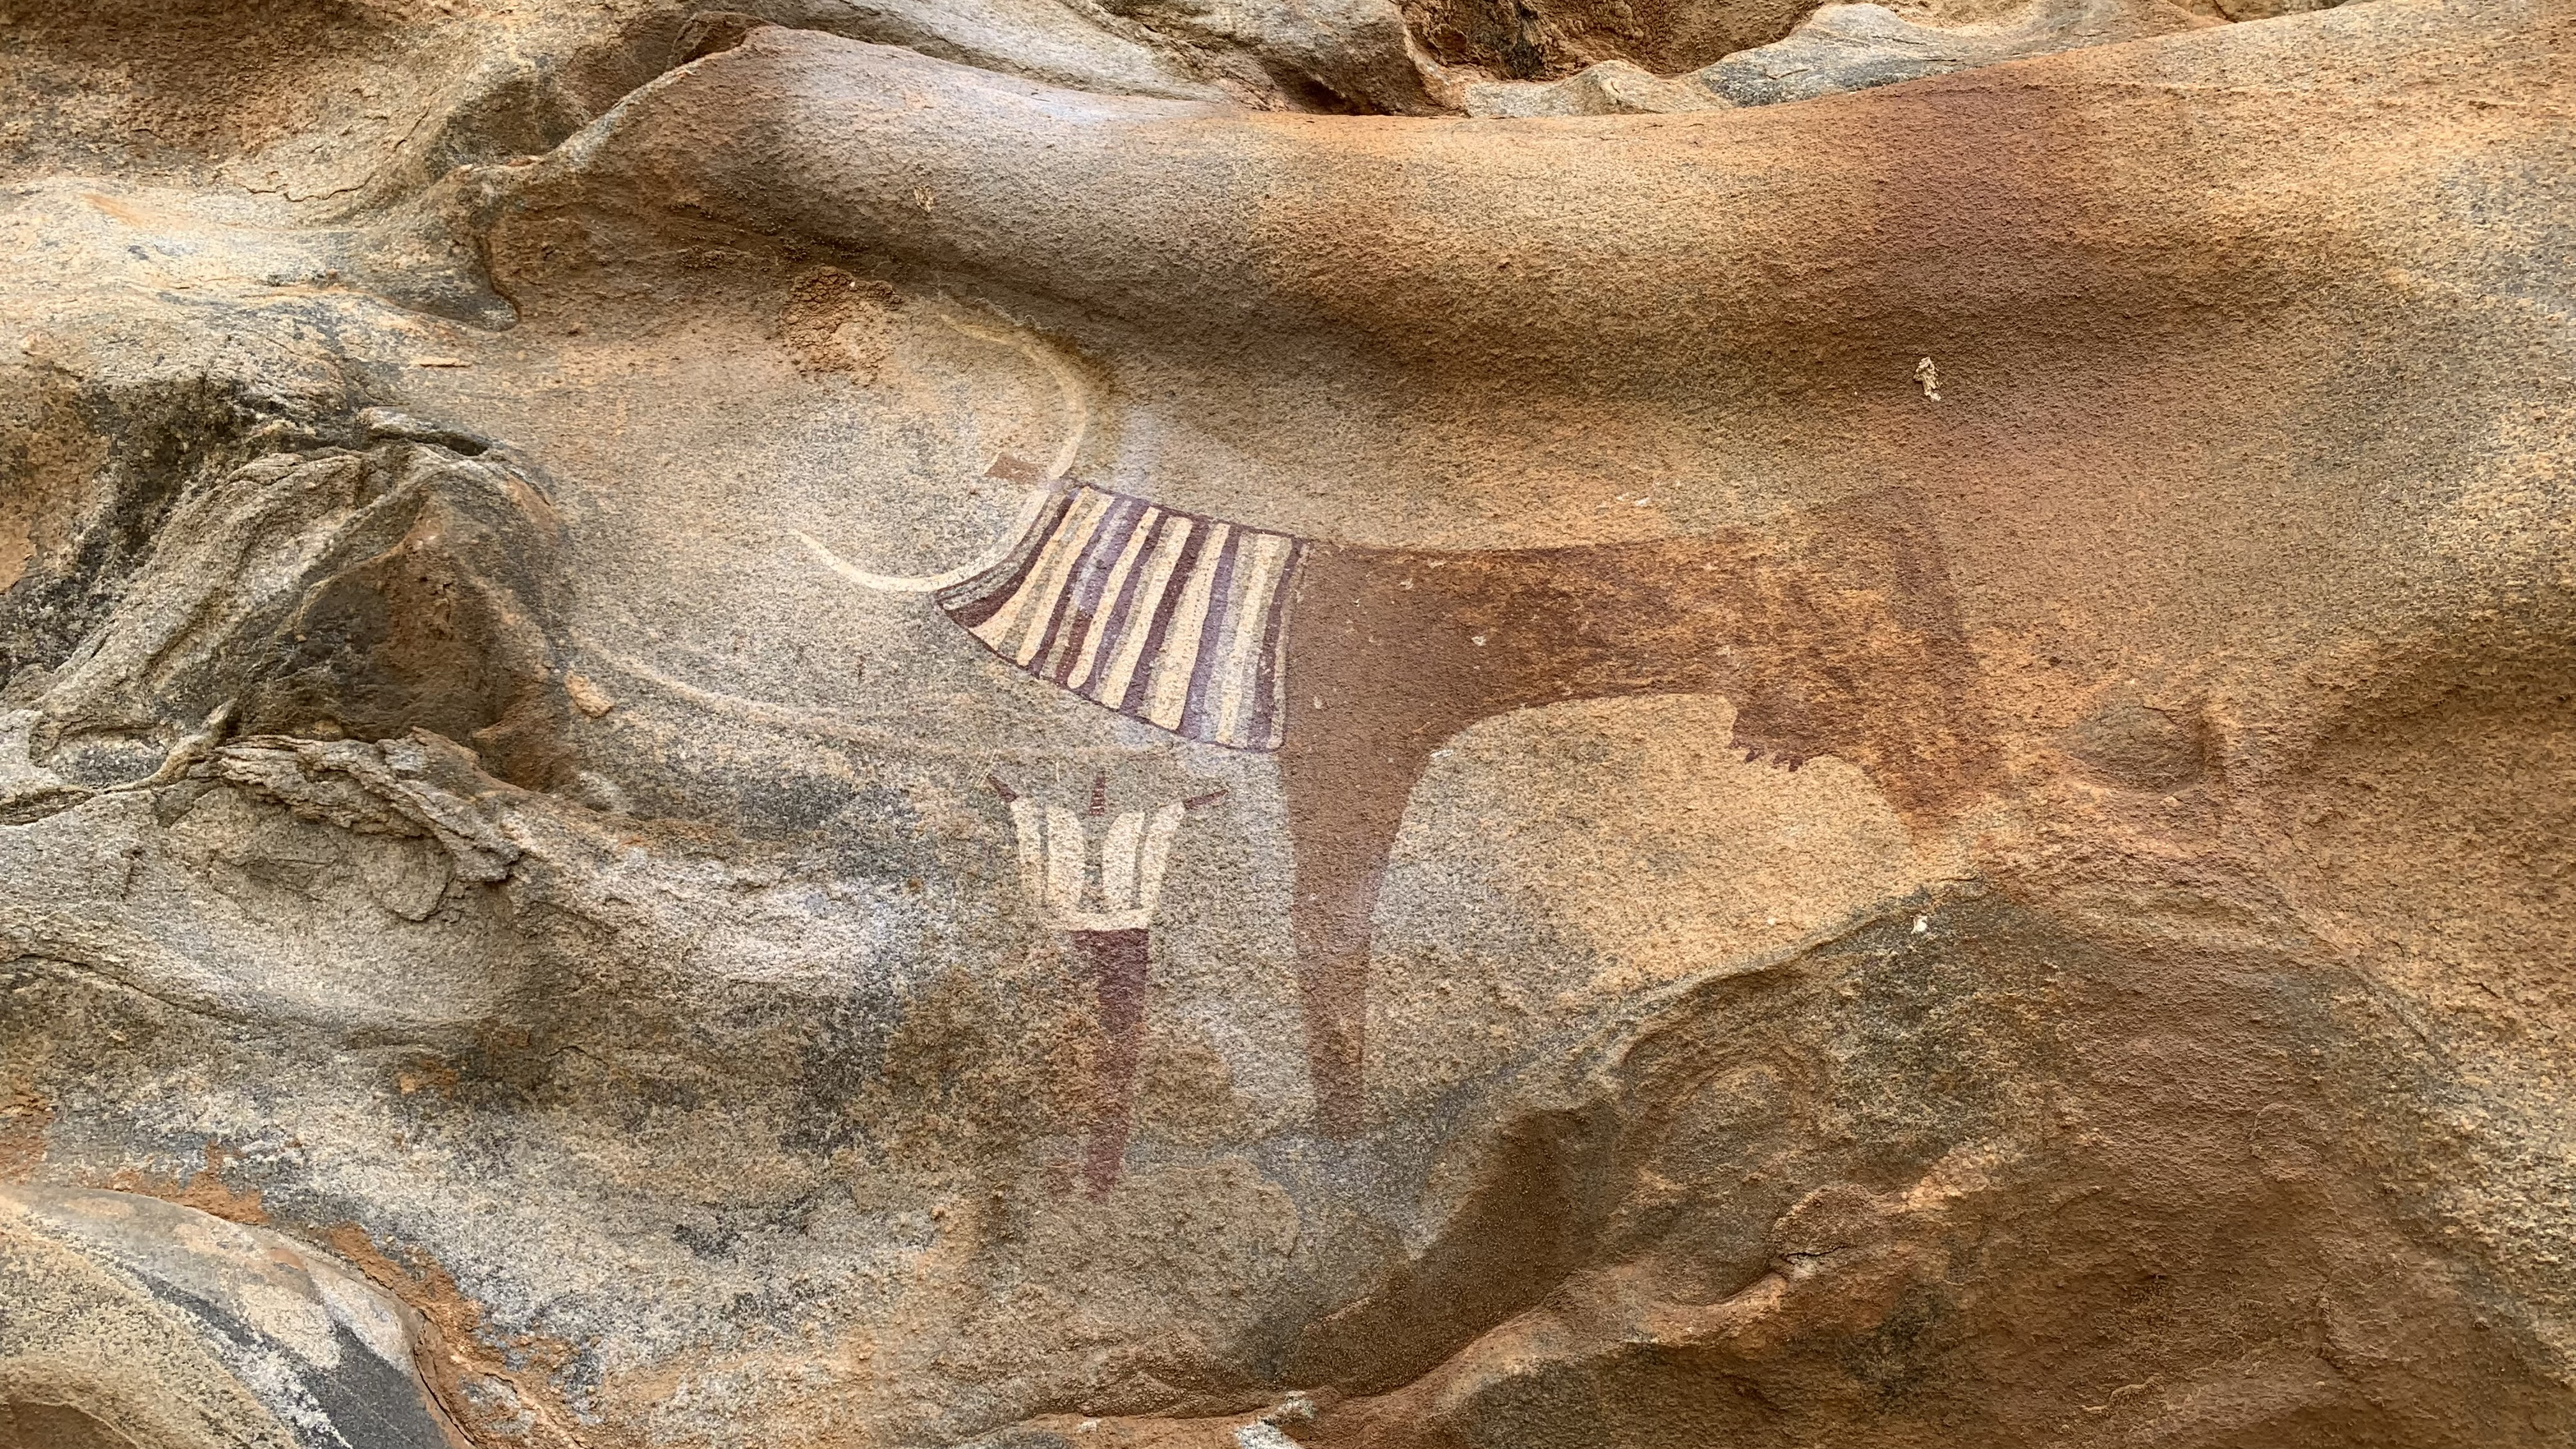
\includegraphics[width=0.45\textwidth]{IMG-5226.jpg}

    \end{center}
    {\small Laas Geel rock art: a big cow with long, curved horns --- she gives birth to calves and gives milk.
    She wears a \textcolor{red}{necklace} because she was the number-one cow of her time.}

\end{frame}

%%%%%%%%%%%%%

\section{Somaliland's Stories}

\begin{frame}{Somaliland patient stories}
    \begin{center}
    \includesvg[width=0.35\textwidth]{TMWH_logo_TAIPEI_vector.svg} 
    \includesvg[width=0.45\textwidth]{Hargeisa_Group_Hospital_logo(1).svg} 
%    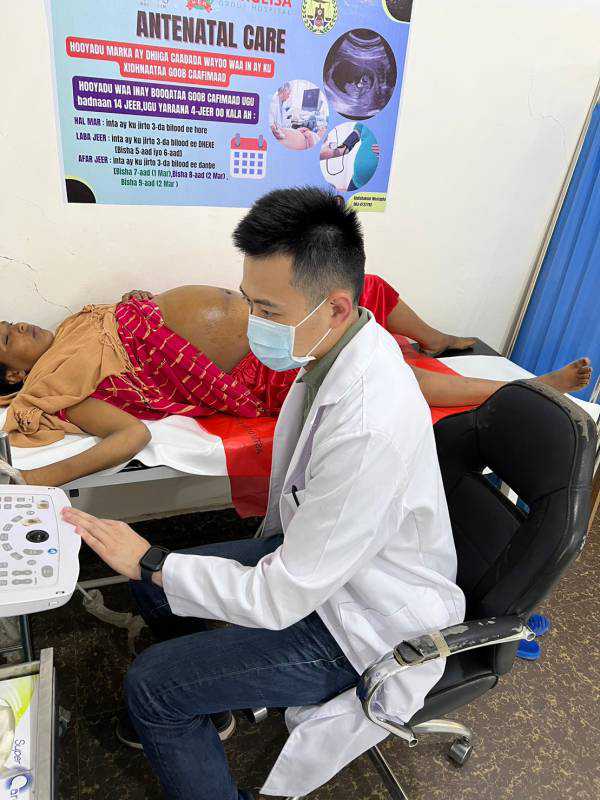
\includegraphics[width=0.3\textwidth, trim=60mm 60mm 30mm 60mm,clip]{52165_antenatal_check.jpg}

\end{center}
\end{frame}

%% ultrasound baby
\begin{frame}
\frametitle{Nimco, happy mother first "see" her baby}
% Add content here
\begin{center}
    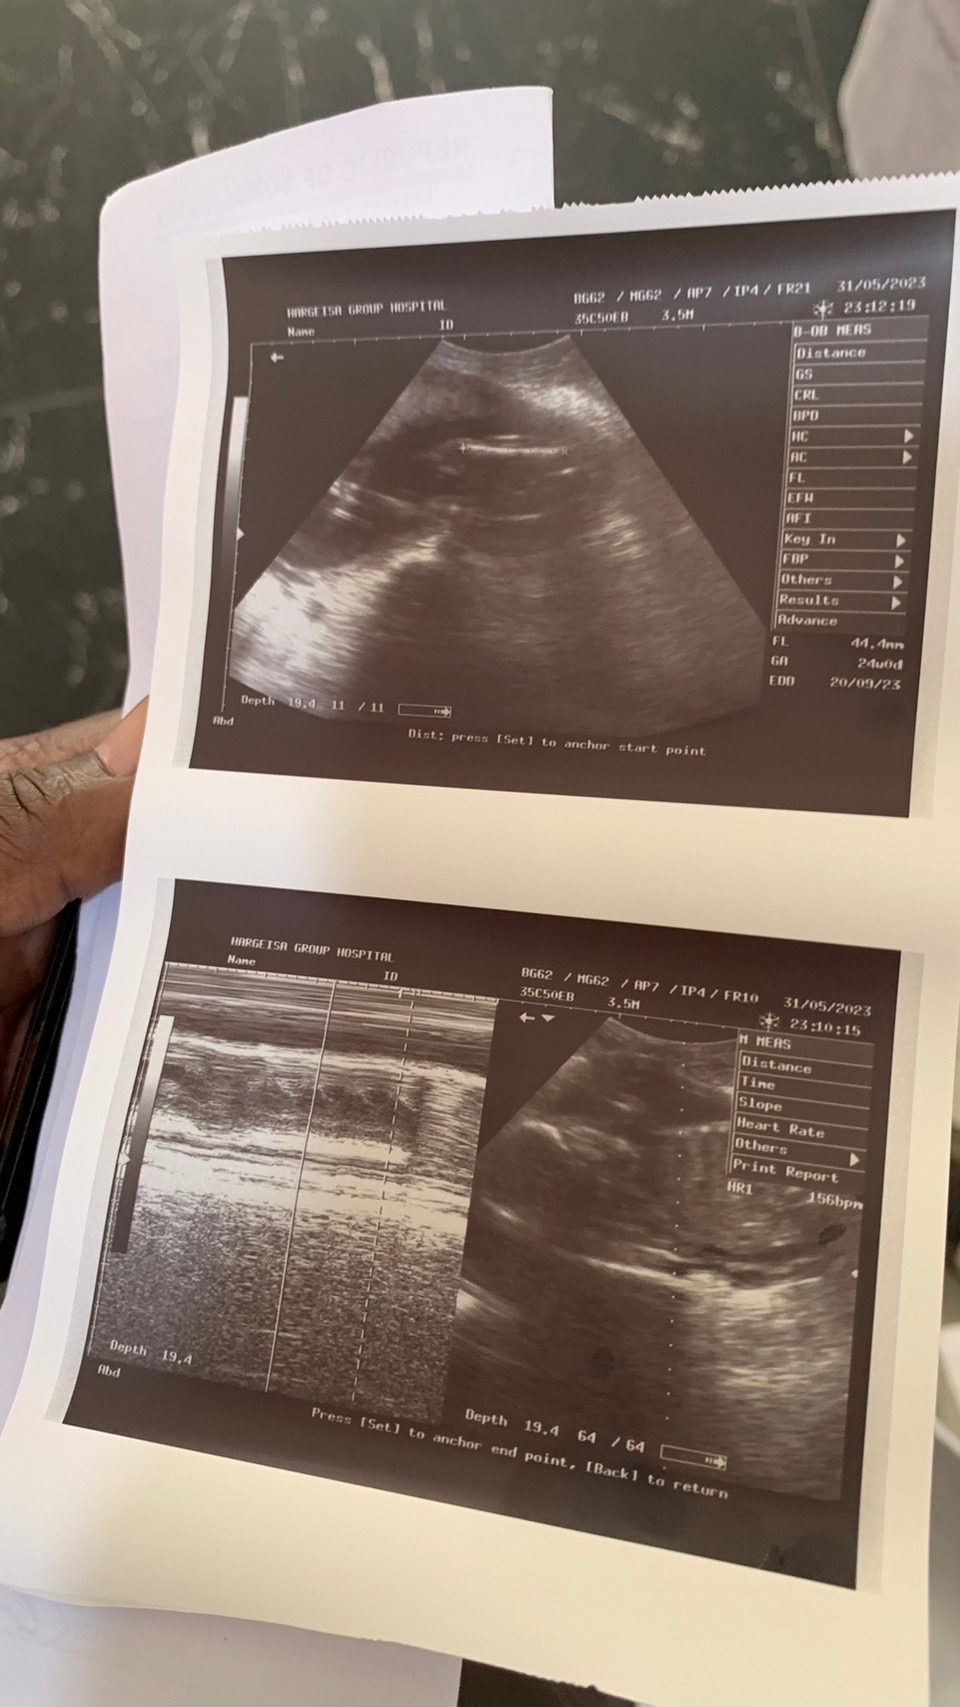
\includegraphics[width=0.3\textwidth, trim=00mm 100mm 00mm 60mm,clip]{IMG-5117.JPG} 
    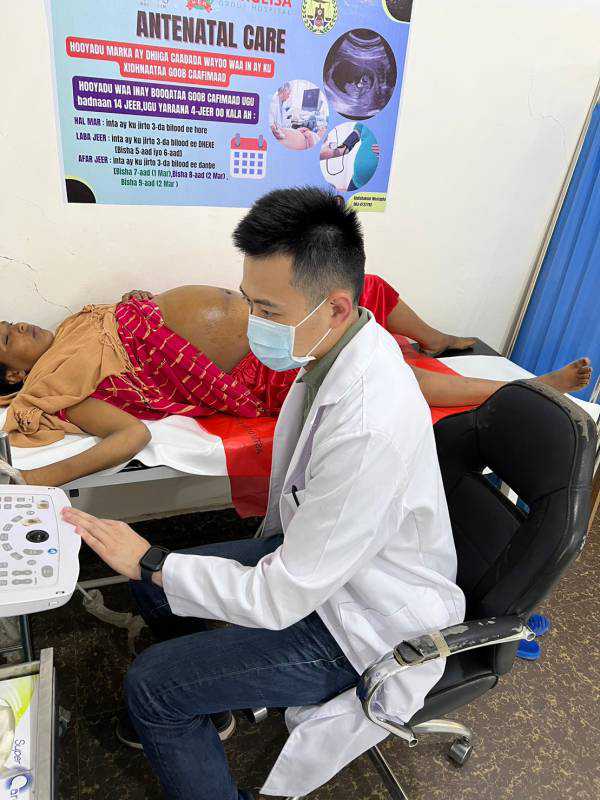
\includegraphics[width=0.3\textwidth, trim=60mm 60mm 30mm 60mm,clip]{52165_antenatal_check.jpg}

\end{center}
\end{frame}

%% Ismail oral cancer
\begin{frame}
\frametitle{Ismail said, "Welcome, I'm going to sleep."}
% Add content here
\begin{center}
\raisebox{70mm}{
    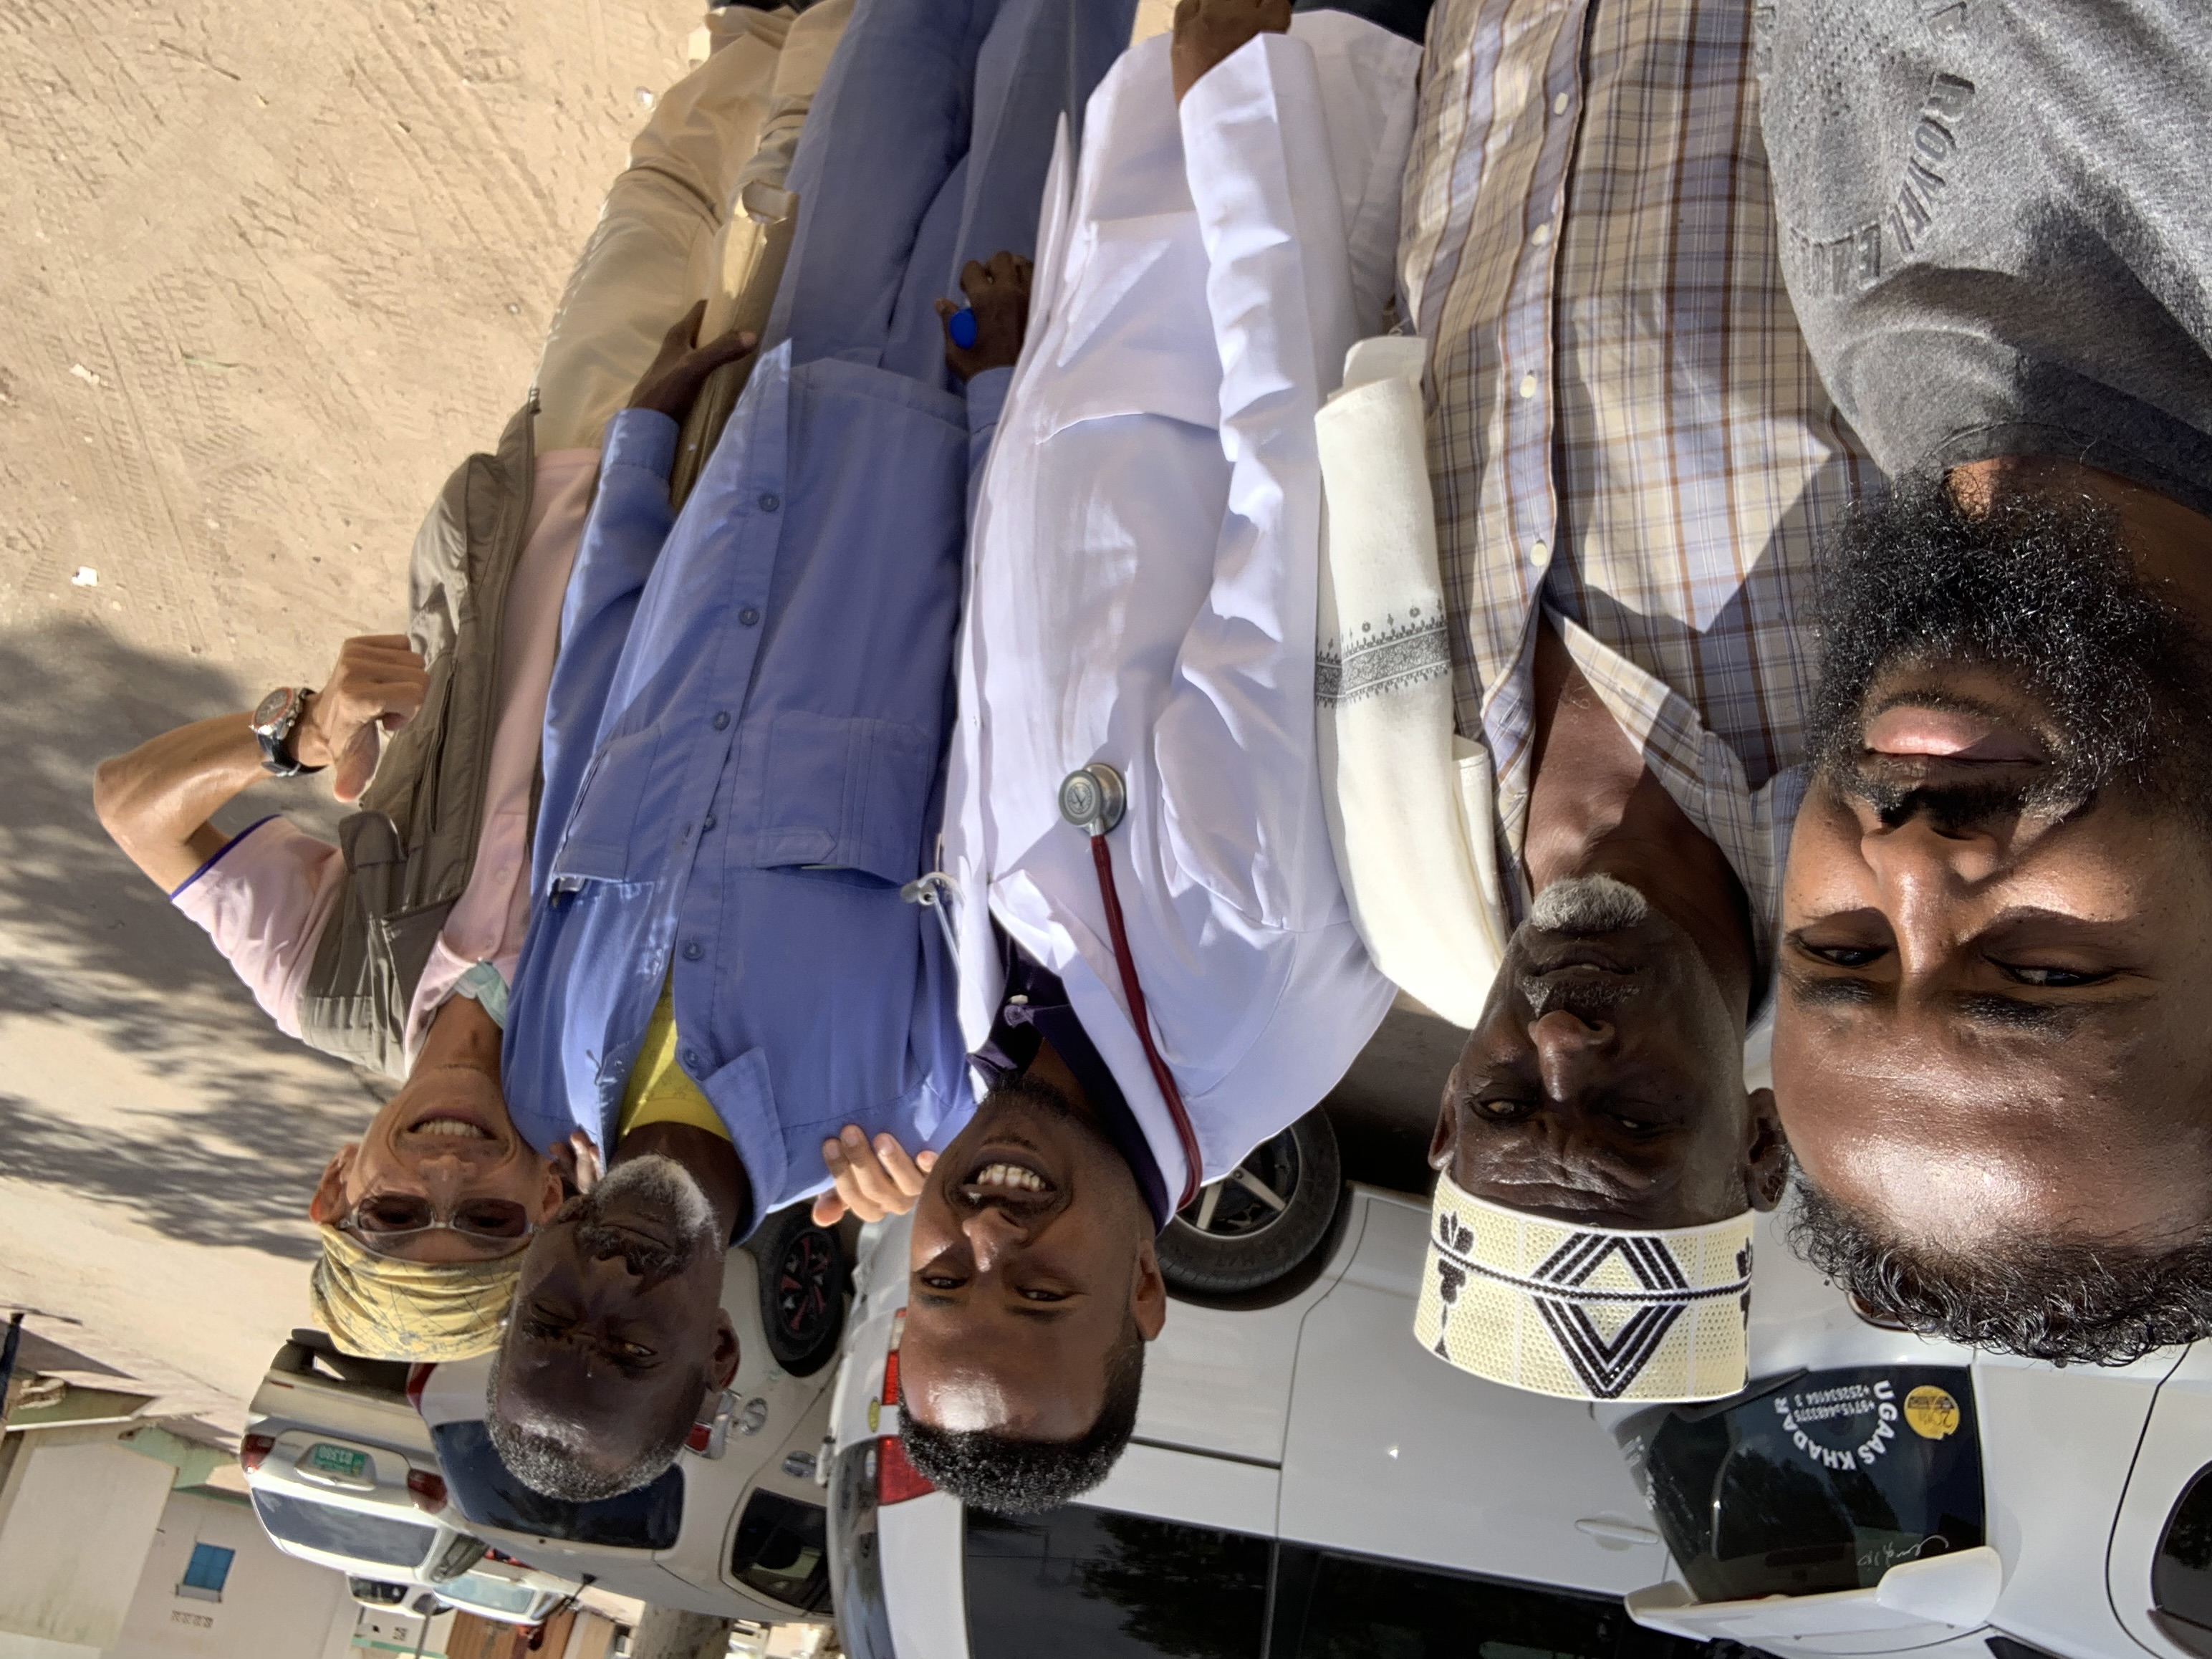
\includegraphics[width=0.8\textwidth, scale=-1,angle=180]{IMG-4861.jpg} 
    }
%    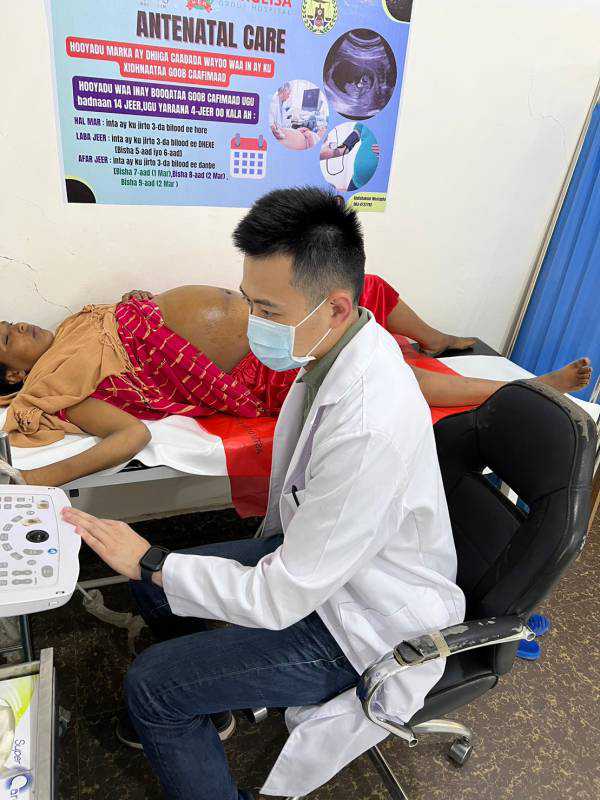
\includegraphics[width=0.3\textwidth, trim=60mm 60mm 30mm 60mm,clip]{52165_antenatal_check.jpg}

\end{center}
\end{frame}

%%%%%%%%%%
\section{Conclusion}
\begin{frame}
\frametitle{Thanks all of TMM members (2022, 2023, 2024, 2025, 2026, ...)}
% Add content here
\begin{center}
\raisebox{90mm}{
    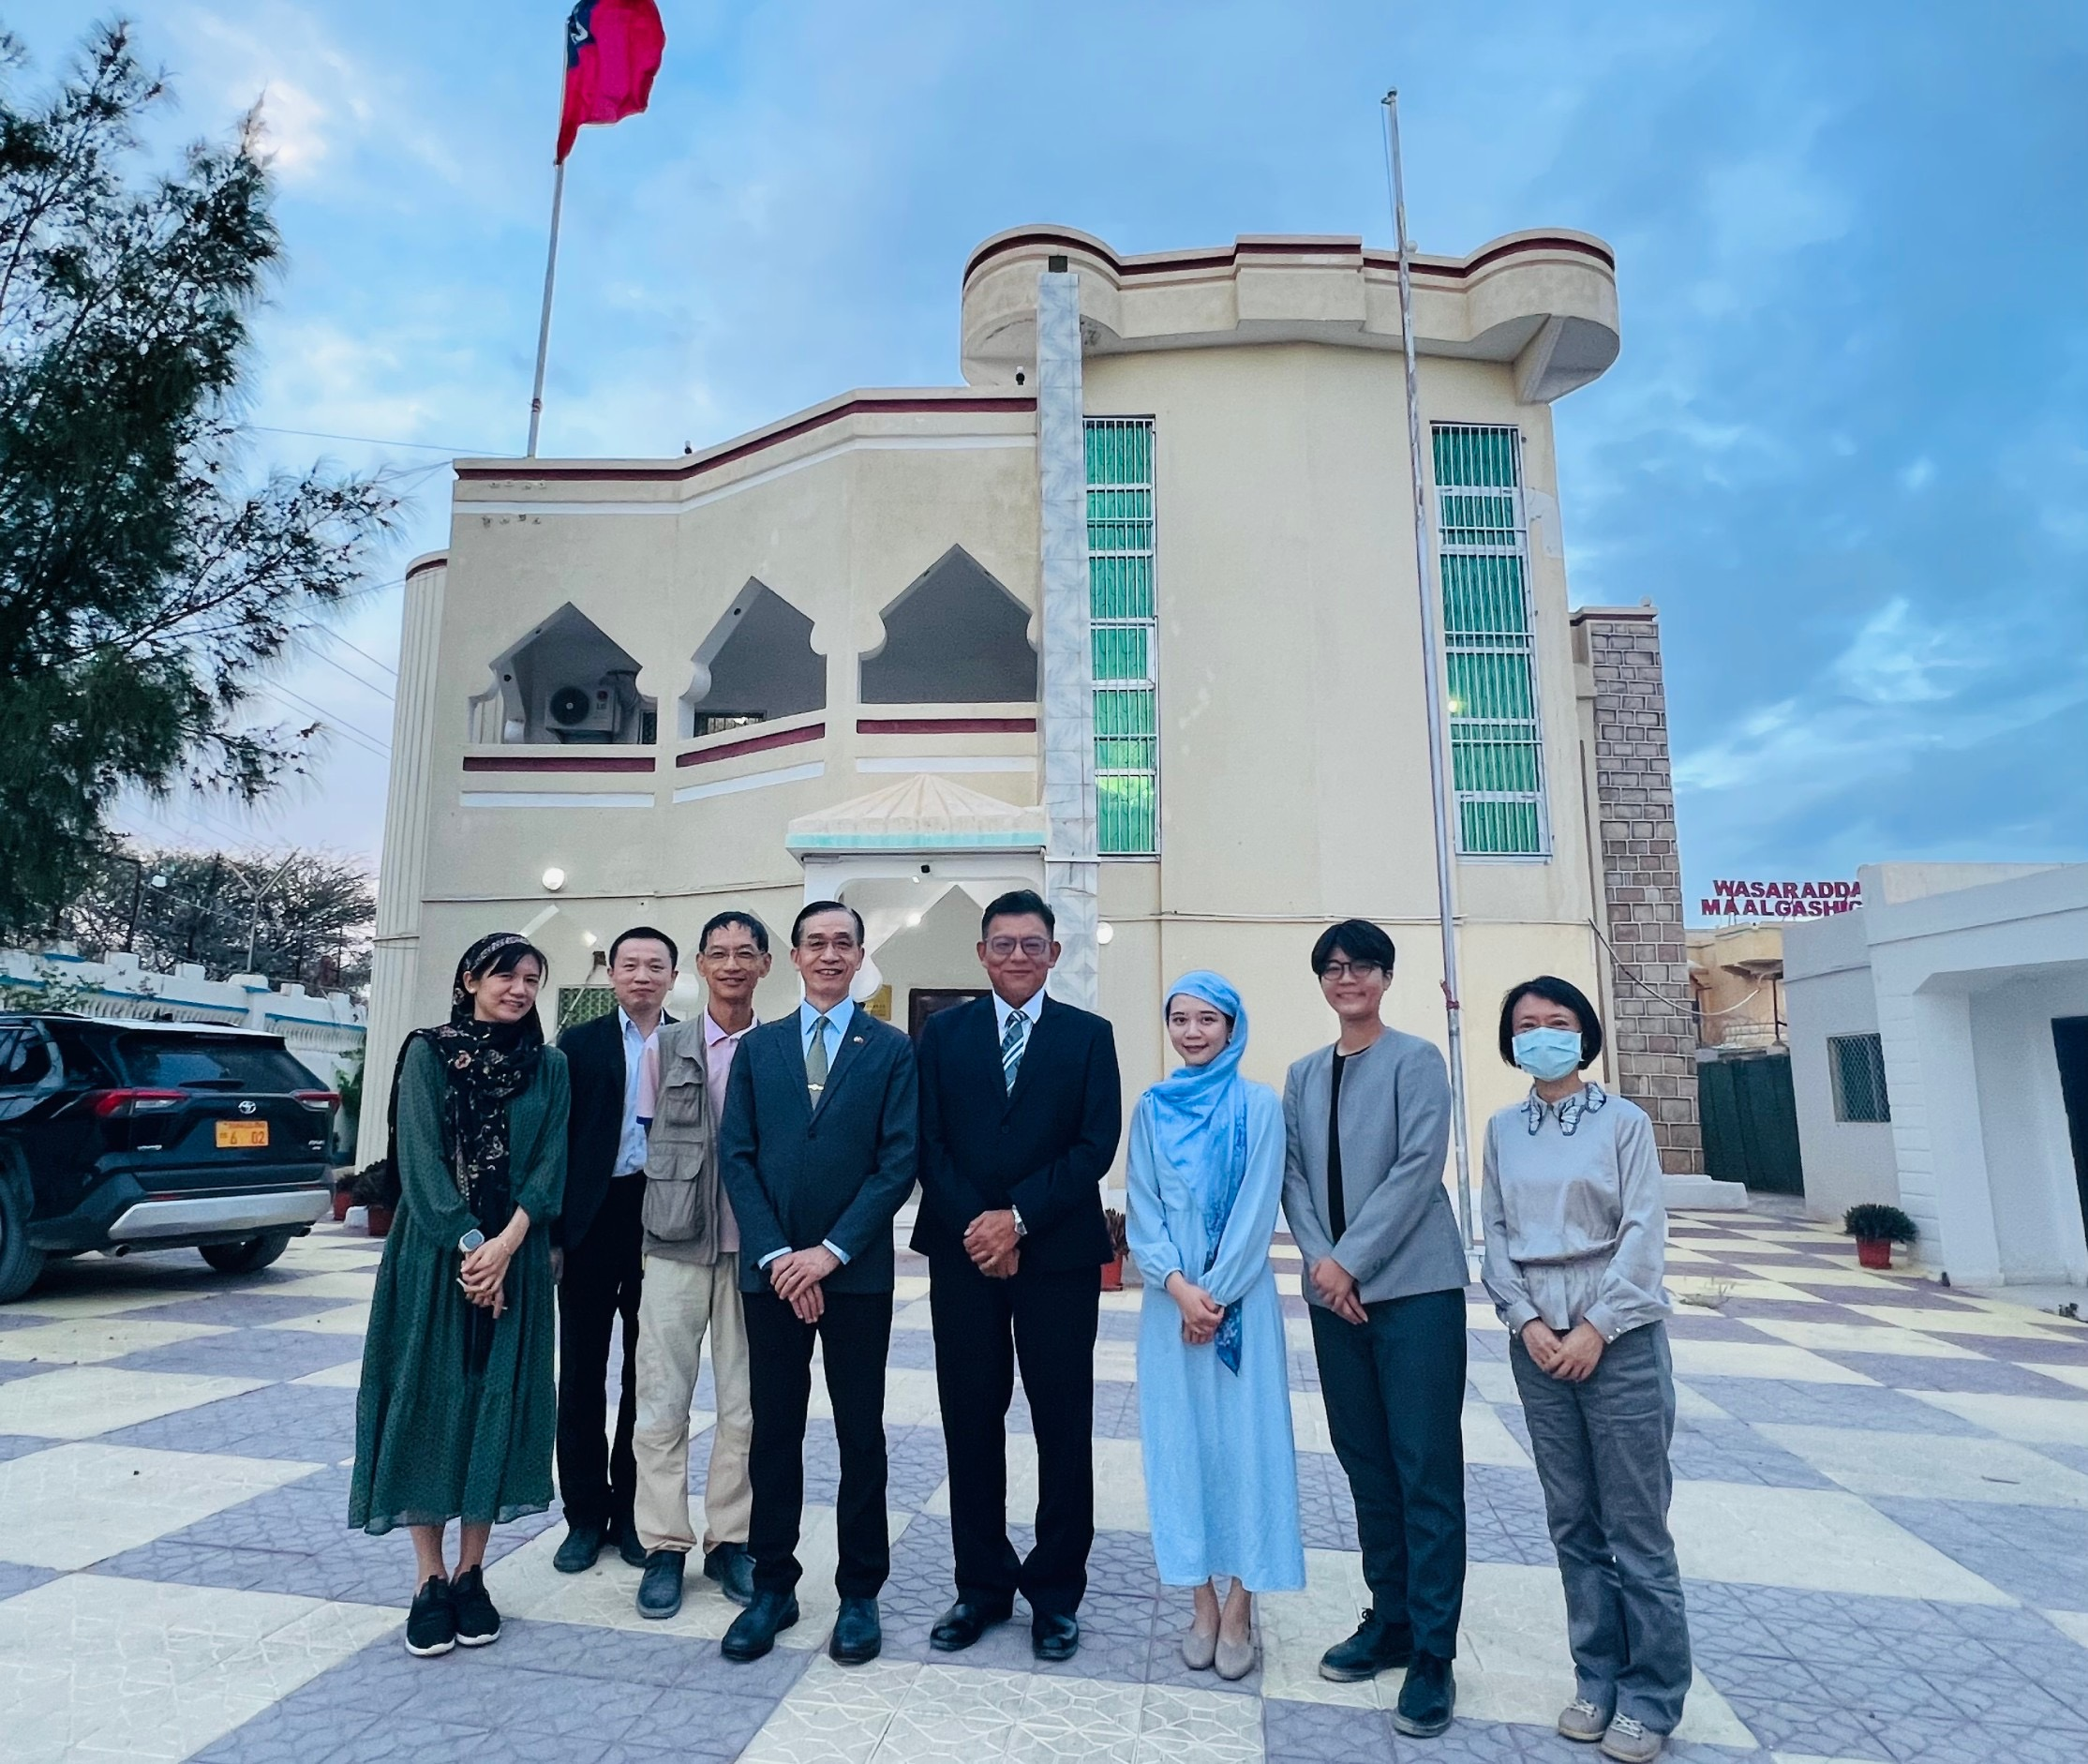
\includegraphics[width=0.5\textwidth]{IMG-5017.JPG} 
    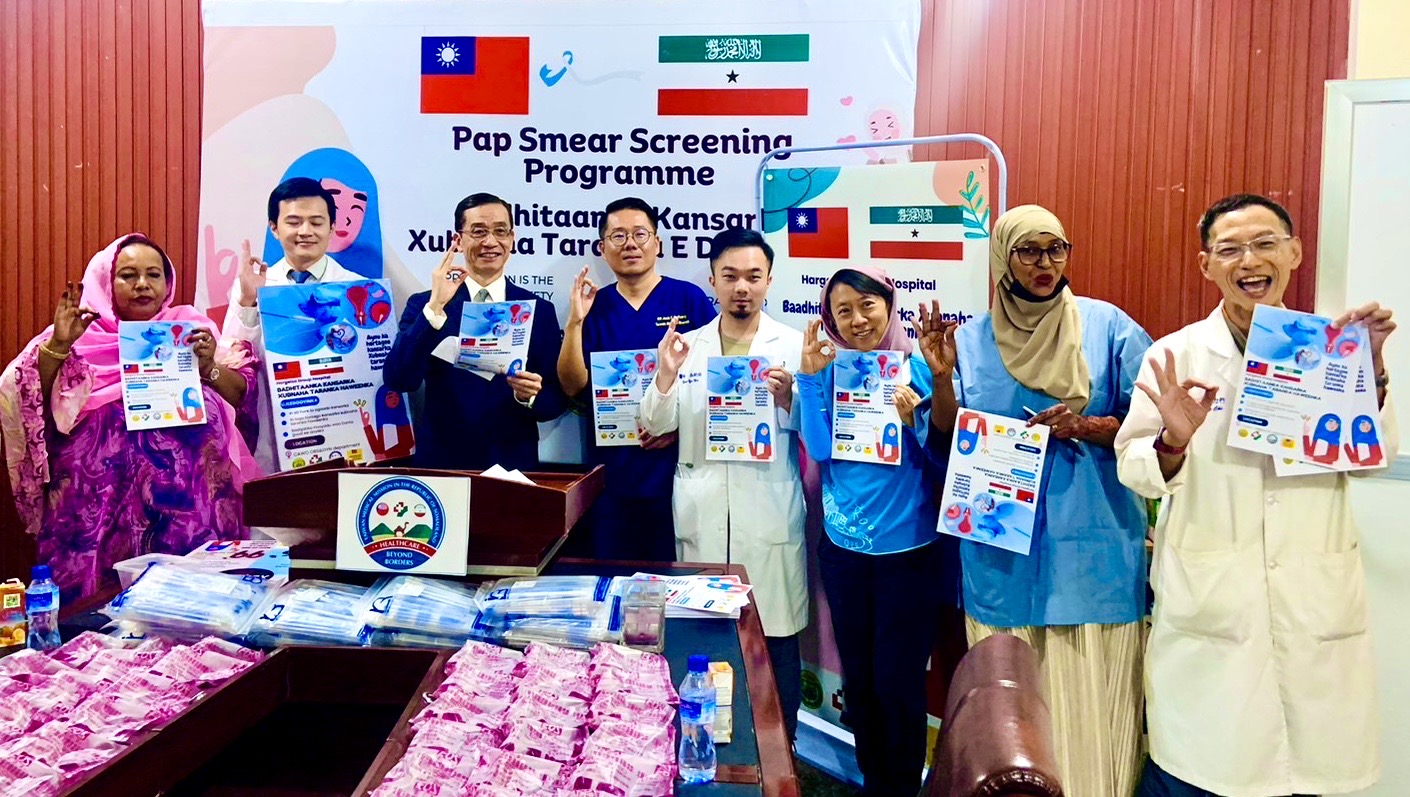
\includegraphics[width=0.5\textwidth]{IMG-5437.JPG} 
    }
%    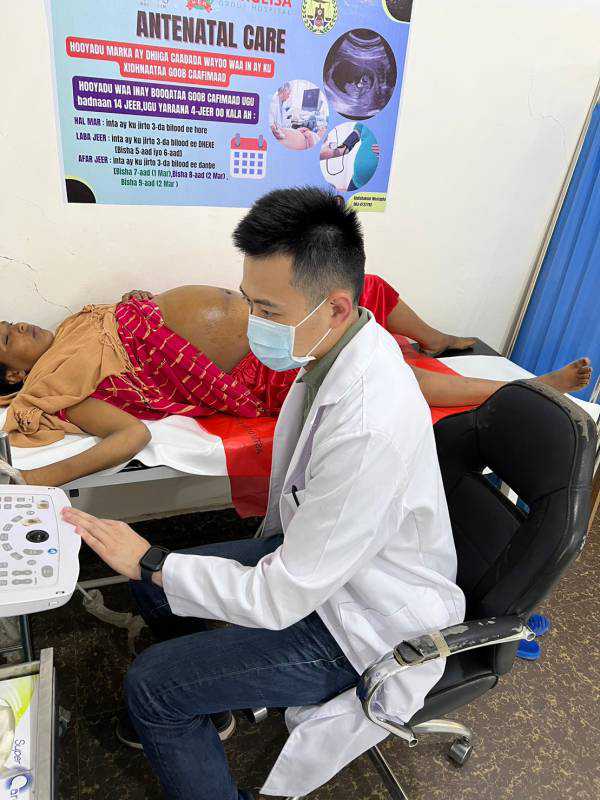
\includegraphics[width=0.3\textwidth, trim=60mm 60mm 30mm 60mm,clip]{52165_antenatal_check.jpg}

\end{center}
\end{frame}


%%
\begin{frame}{How to prepare for global health nursing}
\vspace*{-0.9em}
\small
\begin{outline}
\1 \textbf{Become an experienced RN first} --- the medical mission needs nurses with experience.
    \2 {\footnotesize\color{gray}醫療團要等到護理師有經驗之後}
\1 \textbf{Start now in student groups} --- build international experience while you study.
    \2 {\footnotesize\color{gray}學生團體就能開始累積國際經驗}
\1 \textbf{Use English every day} --- in an English environment your listening grows fast; this EMI class is your start.
    \2 {\footnotesize\color{gray}身處英語環境，聽力自然會大幅成長}
\1 \textbf{Compassion, empathy, friendship, adaptability} --- and be ready to \textcolor{red}{learn from them}.
    \2 {\footnotesize\color{gray}有愛心、同理心、愛交朋友，能隨遇而安}
\1 \textbf{AI capability} --- use LLMs and AI tools for speed and quality; English writing is no longer a barrier for non-native speakers.
    \2 {\footnotesize AI is a \textcolor{red}{friend}: we work together and learn from each other --- met by 緣, kept by 愛.}
    \2 {\footnotesize\color{gray}善用 AI 提升速度與品質；AI 是人類的朋友，一起工作、互相學習。}
\end{outline}
\end{frame}

%%
\begin{frame}
\frametitle{Take Home Message}
% Add content here
\begin{columns}
    
\column{0.4\textwidth}


\begin{outline}
 %   Our core value is:
TMM is writing Somaliland's medical history \\
{\footnotesize\color{gray}TMM正在撰寫索蘭的醫療史}
\1 Teaching {\color{gray}教學}
\1 Service {\color{gray}服務}
\1 Public health {\color{gray}公衛}

%\1 TMM offers medical professionals for people in need.
%\1 TMM's presence is supposed to bring happiness and safety to everyone around them
%iby improving their health and well-being.
%\1 TMM members have confidence, resilience, determination, and empathy when they face challenges.
\end{outline}

\column{0.6\textwidth}
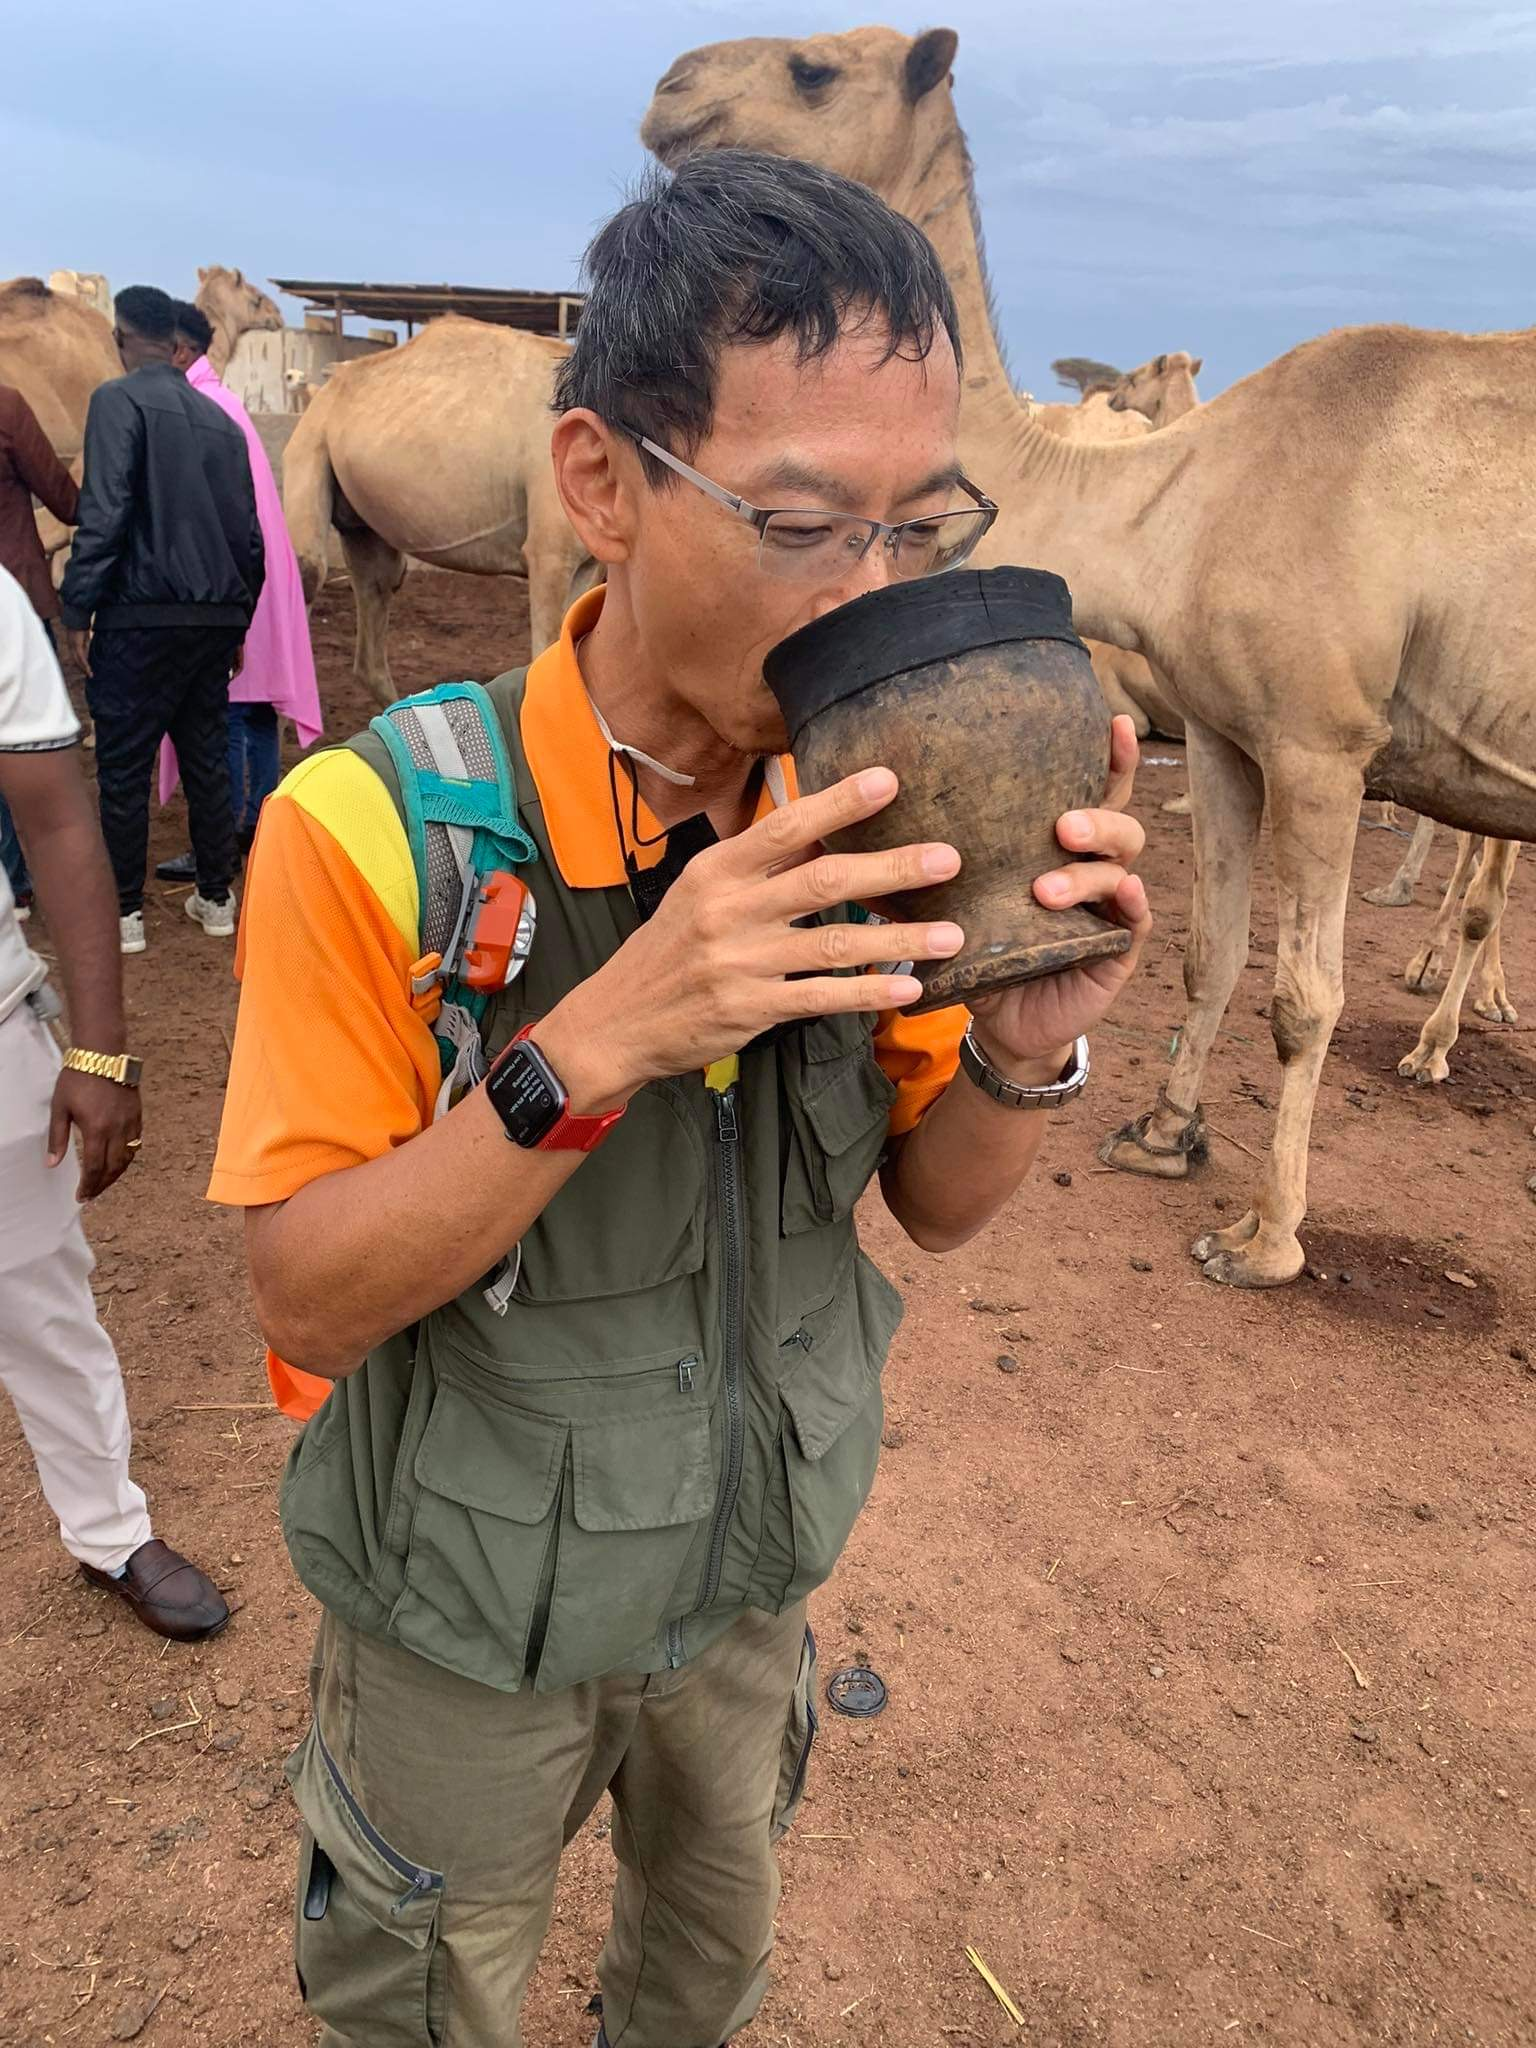
\includegraphics[width=0.6\textwidth]{IMG-0394.JPG}
\end{columns}
\end{frame}

\begin{frame}{Trust me, Trust you}

\begin{columns}
    
\column{0.4\textwidth}
\begin{outline}
%Whenever TMM's members have short-term or long-term work in Somaliland,

%\1 TMM members work as a team in Somaliland, whether they are there for a short time or for a long time.
\1 You can, however, think about how you can use the skills and experiences \textcolor{red}{you learned from here} in your future job and life in Taiwan.
%\1 You can make the most of this time as a chance to learn and grow so that you can help us all get
%through \textcolor{blue}{the challenges} that we face here. 
%\1 We think that constant help is important for our overseas mission to be successful.

\end{outline}

\column{0.6\textwidth}
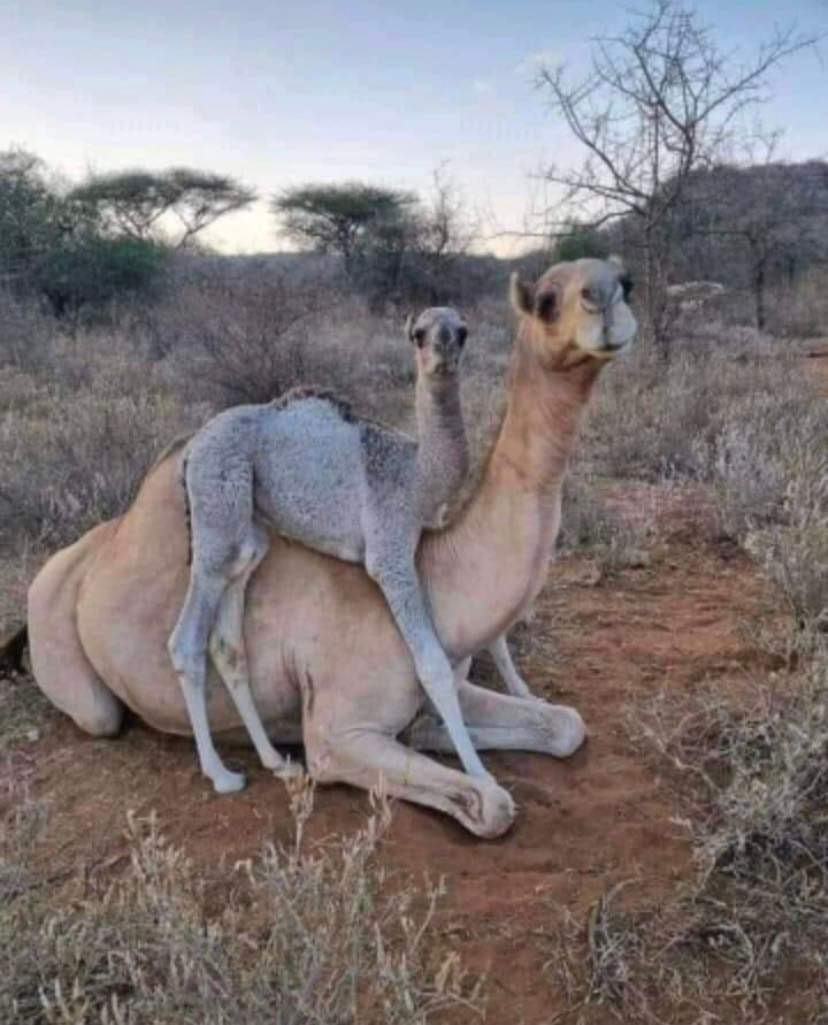
\includegraphics[width=0.7\textwidth]{IMG-5113.JPG}
\end{columns}

\end{frame}
%%

\begin{frame}{Outreach}
    \begin{columns}
    to community (IDP site C)
    \column{0.6\textwidth}
    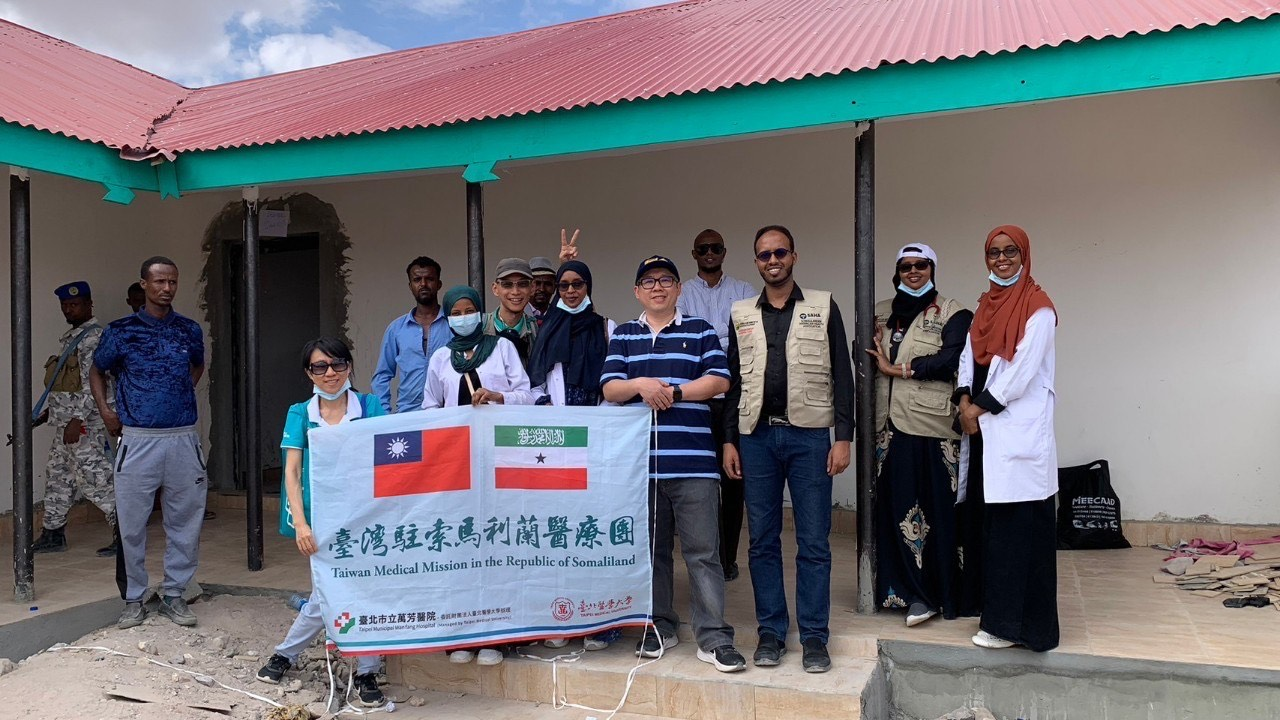
\includegraphics[width=0.7\textwidth]{IMG_1713.jpeg}
    \end{columns}  
\end{frame}


%%%
\begin{frame}{Finale}
\begin{columns}
    
\column{0.4\textwidth}
\qrcode[height=2in]{https://www.facebook.com/profile.php?id=100094220689116&mibextid=LQQJ4d}
TMM facebook

\column{0.6\textwidth}
TMU: Passion under the White Coat --- sequel 2026 \\
{\footnotesize\color{gray}TMU 白袍下的熱血—續集 2026}
\small
\begin{outline}
    \1 Human warmth embraces what we cannot change \\ {\scriptsize\color{gray}人性面的溫暖，包容現實層面的無能為力}
        \2 Patients pay for everything themselves --- like Taiwan in the 1970s \\ {\scriptsize\color{gray}看病實況：一切自費，好似 1970 年代的臺灣}
        \2 ``They'' accept death more calmly than ``we'' do \\ {\scriptsize\color{gray}``他們''比起``我們''更能坦然接受死亡}
        \2 \textcolor{red}{Because they have little, they can let go} \\ {\scriptsize\color{gray}因為沒有很多，所以能捨}
    \1 Being a doctor in Africa --- a wonderful experience \\ {\scriptsize\color{gray}當個非洲醫師的經驗，真好}
%娓娓道來 

\end{outline}


\end{columns}
\end{frame}


%\end{CJK*}

%%%
\begin{frame}{Epilogue 尾聲：七言絕句}
\begin{columns}[c]
\column{0.48\textwidth}
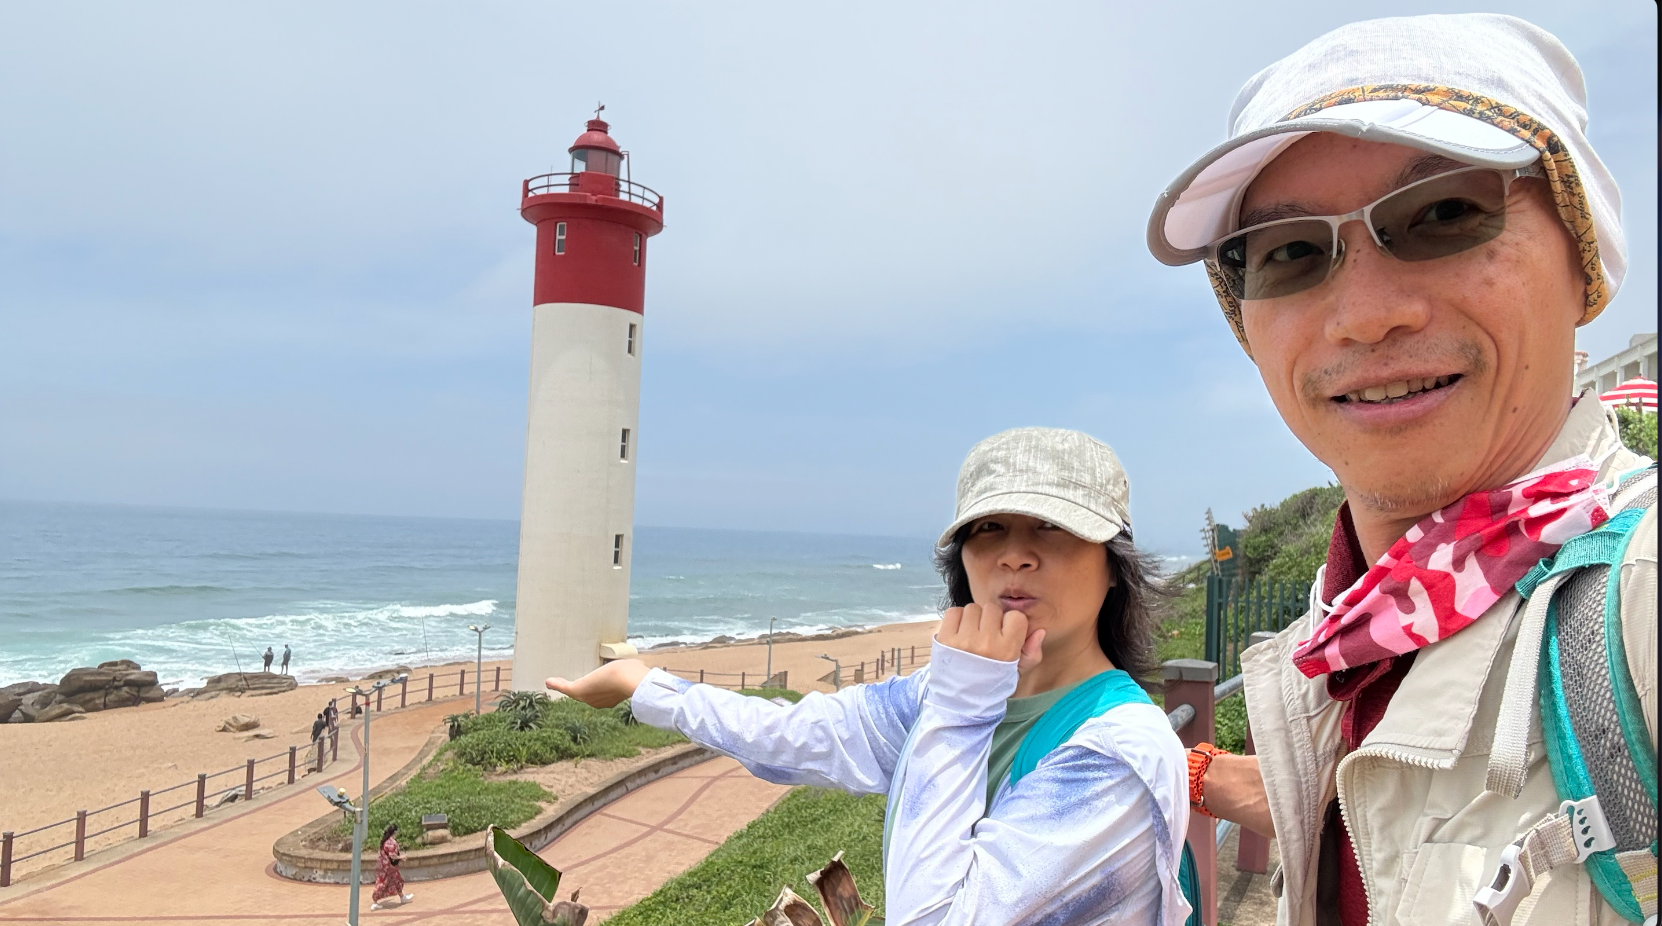
\includegraphics[width=\linewidth]{lighthouse_chi.png}

\column{0.52\textwidth}
\begin{center}
{\large\bfseries 臺灣醫療使命}\\[0.5em]
{\normalsize
寶島醫隊越重洋，\\[0.2em]
索蘭史瓦共翱翔。\\[0.2em]
公衛教學攜手志，\\[0.2em]
臺史共燃智慧光。\\[0.5em]
}
{\footnotesize\color{gray}
Taiwan's medical team crosses the vast ocean;\\
Somaliland and Eswatini, soaring together.\\
Joining hands — public health and teaching as equals;\\
Taiwan \& Eswatini kindle wisdom's light together.\\[0.3em]
TMM Somaliland 2022\\ MMT São Tomé \& Príncipe 2011\\ TMM Eswatini 2008\\[0.2em]
FTM AI Chief 2025
}
\end{center}
\end{columns}
\end{frame}

\end{document}
